\documentclass[12pt]{report}
\usepackage{fancyheadings}
\usepackage[american]{babel}
\usepackage{alltt}
\usepackage{pslatex}
\usepackage{amssymb}
\usepackage{amsfonts}
\usepackage{graphicx}
\usepackage{graphics}

\textwidth  14cm
\textheight 21cm
\topmargin -20pt
\oddsidemargin  20pt
\evensidemargin 20pt

\setlength{\parindent}{0pt}

\setlength{\parskip}{1ex plus0.1ex minus0.1ex}

% copied from the BWP4 docs
\setlength{\headrulewidth}{0.8pt}
\setlength{\footrulewidth}{0.4pt}
\setlength{\headwidth}{\textwidth}

\pagestyle{fancy}

\lfoot{Mark Randles}
\cfoot{}
\rfoot{Edward Ondieki}
\lhead[\thepage]{\textit \rightmark}
\rhead[\textit \leftmark]{\thepage}

\newcommand{\mychapter}[1]{\chapter{#1} \label{ch:#1} \thispagestyle{fancy}}
\newcommand{\bslash}{\verb=\=}
\newcommand{\myitem}[1]{\item{\textbf{#1:}}}
\newcommand{\mycode}[1]{\section{#1} \small{\input{#1}} \newpage}

\newsavebox{\tempboxa}
\newenvironment{file}[1]{ \textbf{File:} \texttt{#1} \\ \label{file:#1} \nobreak \hrule \begin{alltt} }{ \end{alltt} \hrule \vspace{0.5cm} }
\newenvironment{code}[2]{ \textbf{Code:} \texttt{#1} \\ \label{code:#2} \nobreak \hrule \begin{alltt} }{ \end{alltt} \hrule \vspace{0.5cm} }

\begin{document}
\bibliographystyle{plain}

% title page
\begin{titlepage}
\vspace{9cm}
\begin{center}
    \huge Synchronous Relaxation and Time Warp Algorithms: A Study
\end{center}
\vspace{1.0cm}

\vspace{1cm}

\vspace {1cm}
\centerline{
\begin{tabular}{cc}
Mark Randles & Edward Ondieki \\
randlem@bgsu.edu & edwardo@bgsu.edu \\
\end{tabular}
}
\vspace{1cm}
\centerline{Academic Supervisor}
\centerline{Hassan Rajaei, Ph.D}

\vspace{1cm}
\centerline{\large Department of Computer Science}
\vspace{0.2cm}
\centerline{\large Bowling Green State University, Ohio}
\vspace{0.2cm}
\centerline{\large 07 Tuesday 2005}

\clearpage
\end{titlepage}
% end copy

% abstract page
\begin{abstract}
There were a variety of ideas and goals pursued during the course of this project.  First and foremost was an overriding goal of pulling the problem away from the system that it ran on.  Previous implementations were dependent upon a certain architecture, and thus the system defined the problem size.  This would need to change, the problem must become independent of the architecture.  To do this, a variety of things were looked at.  First we contemplated rewriting the initial work done on synchronous relaxation (SR).  This accomplished it's goal of making the problem size independent of the architecture.  However, there were still bottlenecks inherent in the system, so the use of Time Warp (TW) was studied.  This also should accomplish the goal of making the problem size independent of the underlying architecture.  Also discussed have been the use of logical processes and hybrid OpenMP/MPI mechanisms, on which work has not been done, but initial studies have been undertaken to study their feasibility.
\end{abstract}

% table of contents
\tableofcontents
\newpage
\mbox{}
\newpage
\mychapter{Introduction}

	In order to model physical processes like thin film growth on large areas and long  time scales, more efficient parallel algorithms need to be developed. In this project we first studied a proposed conservative parallel algorithm known as Synchronous Relaxation(SR) algorithm to try and see whether it can be made more efficient. To do this, we rewrote the initial implementation of the algorithm porting from C to C++ . Though the program was slightly more efficient after revision it still was not scalable, that is, it lost its efficiency as more processors were added.
	We then proposed a  new algorithm that would use a distributed simulation technique known as Time Warp. This optimistic algorithm should incur less synchronization costs  than the SR algorithm and should therefore scale better

\section{Monte Carlo Methods}

Monte Carlo methods are numerical techniques often used to calculate integrals by using (pseudo) random  numbers. A good example of this is the calculation of $\pi$ using the following algorithm
  	Monte Carlo for $\pi$
\begin{enumerate}
\item Generate i random number pairs (Xi, Yi) where $0<Xi<1$, $0<Yi<1$.
\item Count number of pairs within the unit circle radius $r=1$
\item $(count of pairs in r=1)/(total pairs) \approx \pi/4$
\end{enumerate}~\cite{ysja:sr}

Monte Carlo methods have also been successfully applied to solving various problems in statistical physics. A classic example is the Ising model used to study the effect of temperature on a ferromagnet~\cite{ae:kmc}.  Initial Monte Carlo algorithms like the Metropolis algorithm worked by randomly selecting an event to occur and accepting or rejecting the event based on a criteria known as the Detailed Balance criteria. However such algorithms proved slow and inefficient for modeling systems at large sizes and time scale as is the case in thin film growth.

\section{Modeling Thin Film Growth Using Kinetic Monte Carlo}

\subsection{Kinetic Monte Carlo}

Kinetic Monte Carlo is a subset of Monte Carlo techniques that has proved successful and efficient in stochastic modeling non-equilibrium systems. Kinetic is derived from the n-fold way algorithm. In this method all the rates of possible events are known beforehand as well as the probability of each rate occurring. Events are then performed and system time incremented stochastically.
Kinetic Monte Carlo is better suited for non-equilibrium systems like thin film growth or the Ising model because
\begin{enumerate}
\item It satisfies the Detailed Balance criteria an important property of stochastic processes.
\item It uses a finite amount of rates that is event rates are precalculated thus reducing computation
\item No events are rejected as opposed to previous algorithms like Metropolis algorithm which suffers from high rejection at low temperatures.
\end{enumerate}

The algorithm follows the following basic steps
\begin{enumerate}
\item Generate a uniformly distributed random number $0<X<1$
\item Use the number $X$ to select an event to occur depending on the probability of that event happening
\item Perform the event (e.g. flip atom or deposit monomer)
\item Generate a new random number $0<Y<1$
\item increment system time using the formula $T=T + log(Y)/(Σ(event rates))$
\item Repeat Step 1 until a stopping condition is equates true
\end{enumerate}

\subsection{Thin Film Growth}
\label{section:Thin Film Growth}

	Thin film growth is the process by which a layer of atoms (monomers) are deposited on a surface (substrate) usually at low pressure and temperature so as to form a surface coverage that is a few atoms thick. The morphology of the thin film formed is highly dependent on various factors such as the rates of different events for example the number of atoms(adatoms,monomers) being deposited as opposed to the rate at which atoms on the surface(substrate) diffuse. Thin film growth also takes place in enormous time scales when considering events at atomic levels i.e atomic vibrations take place at nanoseconds yet it takes hours or minutes to grow a thin film device~\cite{pc:kmc}.
	In our current model we studied a simple growth model known as the Fractal Growth Model. In this model atoms are deposited on the surface of an atom where they may then diffuse along the surface of the substrate. In case a diffusing (or deposited) atom encounters another atom, it reacts to form an island that binds the the atoms to the surface. In case an atom encounters an island(two or more bound atoms) it will be captured by that island.

To model Thin  film growth using KMC the basic data and data structures required are
\begin{enumerate}
\item A two dimensional lattice to act as a height map
\item A monomer list to keep track of the number of monomers as well as their positions on the lattice.
\item The surface diffusion  rates as well as deposition rates
\end{enumerate}

The algorithm proceeds like a standard KMC with the exception of steps 4 and 5.
\begin{enumerate}
\item Generate a random number $0<X<1$
\item Use the number $X$ to select an event to occur depending on the probability of that event happening
\item Perform the event (e.g. deposit monomer)
\item Update the Lattice heights to record change
\item Update the Monomer list in case monomers were captured or added by event
\item Generate a new random number $0<Y<1$
\item Increment system time using the formula $T=T + log(Y)/(Σ(event rates))$
\item Repeat Step 1 until $(total_depositions/(dimension_x * dimension_y))=1$
\end{enumerate}

\begin{figure}
\hrule
\vspace{0.5cm}
\begin{verbatim}
Sample Output
g++ -c lattice.cpp main.cpp synch.cpp comm.cpp mpiwrapper.cpp
ndep=441
time=0.00556387
coverage=1.00227
time=0.00556387
Execution Time=2.2689
**************S**********************************
1 0 0 2 1 0 1 1 0 1 1 1 1 1 1 0 1 1 1 1 1 0
1 0 2 2 0 1 2 1 1 1 1 1 1 1 1 1 1 1 1 0 1 1
1 0 0 2 2 2 1 1 1 1 1 1 1 1 1 1 1 1 1 1 1 1
1 1 1 1 2 2 1 1 1 1 0 0 1 1 2 2 2 1 2 2 1 1
2 0 1 1 2 2 2 1 1 1 2 2 1 2 1 0 1 0 1 2 2 1
0 0 2 2 2 0 1 1 1 2 1 2 2 1 1 3 1 1 2 2 0 0
0 0 1 1 2 2 1 1 0 1 1 0 2 2 3 1 0 1 1 2 0 1
1 1 1 1 1 0 1 1 1 1 1 1 2 1 3 1 0 1 1 0 1 2
2 1 1 2 1 1 2 1 1 1 1 0 1 1 1 2 1 0 0 1 2 1
2 0 2 2 1 2 2 2 1 1 1 1 2 0 1 2 3 1 0 1 2 1
1 0 1 1 1 1 2 2 1 0 2 2 1 0 1 1 2 2 1 2 1 1
2 0 1 1 1 1 1 2 0 1 2 2 2 1 1 1 1 1 1 1 2 0
0 0 1 1 1 1 1 2 1 1 2 0 1 1 1 1 1 1 1 1 0 0
1 0 1 1 2 2 2 1 1 1 1 2 2 2 1 0 1 1 1 0 1 0
2 0 0 2 1 2 1 1 2 1 0 2 0 1 0 1 1 1 2 2 2 0
2 0 1 0 0 2 2 0 2 2 2 2 1 0 0 2 2 1 2 2 2 1
1 1 2 0 2 1 2 1 2 2 1 1 1 1 2 1 1 2 0 1 1 2
1 2 2 2 1 1 2 2 2 2 1 0 1 1 2 1 2 1 1 0 2 3
1 0 2 1 2 2 1 2 2 2 2 2 2 2 2 2 0 2 1 3 1 1
4 0 1 1 1 0 1 2 2 1 1 0 1 2 2 2 2 2 1 1 4 6
mcount=1
\end{verbatim}
\hrule
\caption{Sample KMC Results}
\label{sampleKMC}
\end{figure}

In Figure \ref{sampleKMC} the bold 3 indicates the presence of a sole monomer on the lattice. This is because it is higher than other heights around it and therefore it does not get bound.  The monomer list contains the location $(X,Y)$ pair of the monomer. In this case the monomer is of size 1 and the $(X,Y)=(9,16)$.



\newpage
\mbox{}
\newpage
\mychapter{Synchronous Relaxation}

\section{Introduction}
The first parallel KMC algorithm we studied was the synchronous relaxation algorithm (SR). The Synchronous Relaxation algorithm was first used to study circuit switched networks. Researchers like Lubachevsky then applied the algorithm to the Ising model and showed that are given a number of weak assumptions, the algorithm is efficient and scalable. The SR algorithm was later adapted by researchers at the University of Toledo to model thin film growth.

The Synchronous Relaxation algorithm is an optimistic algorithm which means that processors can process information independent of each other.
The algorithm works as follows:
\begin{description}
\myitem{Step 1} Each Processor generates KMC events independent of other processors for a cycle time T
\myitem{Step 2} When T expires each processor exchanges information on events that happened to see if any events generated by its neighbor affect it.
\myitem{Step 3} If events in each processor do not affect events in neighbors process, all  processors proceed to the next cycle
\myitem{Step 4} If information received from one neighboring process affects another processor, all processors redo their KMC events incorporating  information gathered.
\myitem{Step 5} Processors again exchange information if events in neighboring processes affect other neighbors Step 4 is repeated. Or else all processors go to next cycle
\end{description}~\cite{ae:kmc}

\begin{figure}
\hrule
\resizebox{\textwidth}{!}{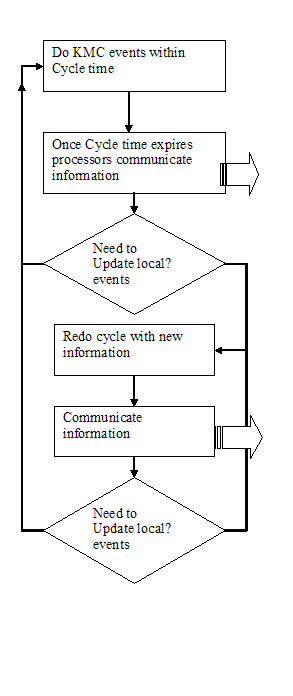
\includegraphics{srright}
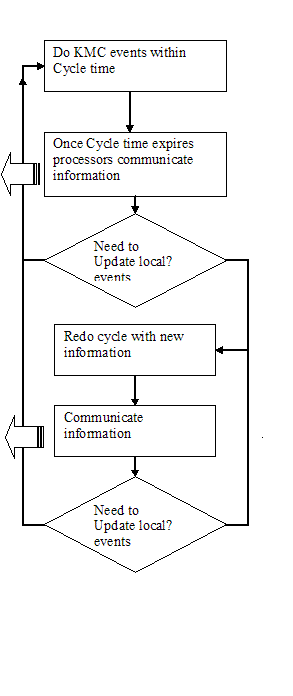
\includegraphics{srleft}}
\hrule
\caption{Synchronous Relaxation Flow Chart}
\end{figure}

\section{Original Algorithm}

\subsection{Boundary Events}
The main problem with parallelizing lattice based KMC problems like thin film growth is that of boundary events. Boundary events are those events that take place on the edge of the lattice and may affect the evolution of neighboring lattices. The SR algorithm is used to try and iteratively correct such errors.

\subsection{Ghost Region}
The ghost region is the area of a lattice that belongs to another lattice but whose events may affect the current lattice. In the initial implementation for the fractal model the Ghost region was one lattice step since diffusions take one step at time.

\subsection{Data Structures}
Modeling KMC events using Lattices can be rather complex. This is because a number of different data structures are required to keep track of the system.

\small{\begin{description}
\myitem{\texttt{h[x][y]}} 2x2 Integer array for the height map. (Appendix \ref{code:sr/lattice.h})
\myitem{\texttt{indexa[size],ipointa[size],indexc[size]}} Three lists to keep track of mobile monomers on the lattice. (Appendix \ref{code:sr/lattice.h})
\myitem{\texttt{myeventlist[size*size]}} An event list to track. (Appendix \ref{code:sr/lattice.h})
\myitem{\texttt{bdyeventlist[size]}} Keeps track of boundary events generated. (Appendix \ref{code:sr/lattice.h})
\myitem{\texttt{ranlist[size]}} list of random numbers generated. (Appendix \ref{code:sr/lattice.h})
\end{description}}

\subsection{Functions}
\begin{description}
\myitem{\texttt{DoKMC}} using a counter this function selected the next random number from the list and used this number to determine which event should take place (diffuse or deposit)
\myitem{\texttt{CalcTime}} calculates the time increment $DT=log(Rand)/sum(event rates)$ and increments the time. It is always called after \texttt{DoKMC()}.
\myitem{\texttt{Diffuse}} This function was called by the \texttt{DoKMC()} function when a diffuse event was selected. The function selects a random location on the lattice and increments it by one. It then calls \texttt{upnbhd()}.
\myitem{\texttt{Deposit}} This function was called by the \texttt{DoKMC()} function when a deposit event was selected. The function selects a random location on the lattice and increments it by one. It then calls \texttt{upnbhd()}.
\myitem{\texttt{Upnbhd}} When a monomer moves (diffuses) or is first deposited this function is called to check whether there are any neighboring monomers or islands that would bind the monomer to the lattice. If there are no monomers or islands surrounding the current monomer then it is added to the list. If there is a monomer/island next to the list then the monomer is deleted from the list or not added in the case of a deposition. If the monomer binds with another monomer that other monomer too will be deleted.
\myitem{\texttt{Undoevent}} This is used in the SR algorithm to undo the events that occurred and restore the list and lattice their state at the beginning of the cycle.
\myitem{\texttt{BufferSendrecv}} This function communicates boundary events to neighboring processes.
\myitem{\texttt{UpdateBuffer}} This function uses boundary events received to correct the lattice. It takes the boundary events received at executes them in order of the time.
\end{description}

\section{Improvements}

\subsection{Multiple Files}
The initial algorithm was implemented in a single C file with a very large number of global variables as well as a large number of functions. To abstract different aspects of the program such as communication functions like buffersendrecv or lattice manipulation functions like diffuse or deposit, we split the program into different files. The function headers where contained in the header files such as \texttt{lattice.h} (Appendix \ref{code:sr/lattice.h}) and implemented in \texttt{lattice.cpp} (Appendix \ref{code:sr/lattice.cpp}) and \texttt{comm.cpp} (Appendix \ref{code:sr/comm.cpp} files.

\subsection{Readability}
In order to work on the existing code we had received we needed to get it more readable. To make it more readable, we first eliminated all global variables. We did this by encapsulating them in a Lattice structure and then passing this structure to functions by reference. This allowed us to follow the execution of the program easier as well add new capabilities to it.

\subsection{Function Overheads}
One of the issues slowing down the execution of the program was excessive function calls. This was taking place especially in the \texttt{Upnbhd()} function where a single call from \texttt{Upnbhd()} would call a helper function eight or more times. By making the small functions inline this helped reduce execution time.
Rewinding to first boundary event

One of the main problems with the initial implementation is that when the program entered the correction phase it had to return to the beginning of the cycle as opposed to correcting after the first boundary event. This therefore increased the computation time and cut the parallel efficiency of the program.
In order to make it possible for the program to rewind to the first boundary event, all changes made to the monomer lists would have to be recorded and then undone. This meant adding extra data structure known as \texttt{ListChange[]}. \texttt{ListChange[]}  kept track of all the insertions and deletions that took place in the monomer list. \texttt{ListChange[]} also kept track of time each of these changes occurred. When the program synchronized and tried to  correct errors from boundary events, it would loop through the \texttt{ListChange[]} structure and restore the list to the state it was at the time of the first boundary event.

\subsection{Results}
The results from the improvements we made were mixed. When function overhead was reduced, the execution time was reduced.   The results are contained in Table \ref{table:Function Overhead}

\begin{table}
\begin{tabular}{|l|l|}
\hline
Execution Time with function overhead (Sec) & Execution Time without function overhead (Sec) \\
\hline
138.16 & 109.12\\
\hline
\end{tabular}
\caption{Execution Time vs. Function Overhead}
\label{table:Function Overhead}
\end{table}

The rewind to first boundary events did not increase parallel efficiency or reduce execution time due to  the complexity of manipulating the three monomer lists. This complexity made the procedure complex and error prone. Execution time was actually increased due to these changes.   The results are contained in Table \ref{table:Rewind List}

\begin{table}
\begin{tabular}{|l|l|}
\hline
Execution Time without rewind list (Sec) & Execution Time with function overhead (Sec) \\
\hline
138.16 & 119.12\\
\hline
\end{tabular}
\caption{Execution Time vs. Rewind List usage}
\label{table:Rewind List}
\end{table}

\subsection{Analysis}
Overall the Changes made to the initial program did not adequately improve the performance of the implementation. The main factors that controlled efficiency where the cycle time, lattice size and diffusion/deposition rates.  For example reducing the cycle time to 10e-6 s with a diffusion/deposition rate of 10e6.  The results are contained in Table \ref{table:Cycle Time}

\begin{table}
\begin{tabular}{|l|l|}
\hline
Execution Time in Sec & Execution Time in Sec \\
Cycle Time=10e3 & Cycle Time=10e6 \\
Diffusion/Deposition=10e5 & Diffusion/Deposition=10e5 \\
\hline
138.16 & 90.12\\
\hline
\end{tabular}
\caption{Execution Time and Cycle time}
\label{table:Cycle Time}
\end{table}

Parallel efficiency was difficult to measure in the initial program because we relied on the OSC cluster and any requests for more than 4 processors resulted in a long queue that could take hours or weeks before a turnaround.

%\subsection{Multiple Files}
%The initial algorithm was implemented in a single C file with a very large number of global variables as well as a large number of functions. To abstract different aspects %of the program such as communication functions like buffersendrecv or lattice manipulation functions like diffuse or deposit, we split the program into different files. The %function headers where contained in the header files such as lattice.h and implemented in lattice.c and comm.c files.

%\subsection{Readability}
%In order to work on the existing code we had received we needed to get it more readable. To make it more readable, we first eliminated all global variables. We did this by %encapsulating them in a Lattice structure and then passing this structure to functions by reference. This allowed us to follow the execution of the program easier as well %add new capabilities to it.

%\subsection{Function Overheads}
%One of the issues slowing down the execution of the program was excessive function calls. This was taking place especially in the Upnbhd() function where a single call from %upnbhd would call a helper function eight or more times. By making the small functions inline this helped reduce execution time.
%Rewinding to first boundary event

%One of the main problems with the initial implementation is that when the program entered the correction phase it had to return to the beginning of the cycle as opposed to correcting after the first boundary event. This therefore increased the computation time and cut the parallel efficiency of the program.
%In order to make it possible for the program to rewind to the first boundary event, all changes made to the monomer lists would have to be recorded and then undone. This meant adding extra data structure known as listchange[]. ListChange[]  kept track of all the insertions and deletions that took place in the monomer list. ListChange[] also kept track of time each of these changes occurred. When the program synchronized and tried to  correct errors from boundary events, it would loop through the listChange[] structure and restore the list to the state it was at the time of the first boundary event.

\subsection{Implementing the Program in C++}
\subsubsection{Motivation}
The motivation for moving the algorithm from C to C++ where
\begin{enumerate}
\item It allowed for a much better abstraction of the program
\item Lattice object would allow for process-processor independence
\item The Lattice class could be reused easily in other algorithms like Time Warp
\item Easier to debug
\end{enumerate}

\subsubsection{Lattice Object}
The lattice Object was now made up of an array of Sites. Each site contained information about its location, height and if a monomer was present the location of that monomer on the monomer list.

\begin{code}{Site and Lattice Object}{sitelattice}
Class Site
\{
    int index;//location of monomer on the monomer list
    int height;
    point position;
\}

Site Lattice[X][Y];//lattice object.
\end{code}

The main advantages of this approach was that it simplified the updating of monomer lists. This meant that we could implement a rewind list easier since there is only ONE list to worry about.

\subsubsection{Multiple files}
Moving from C to C++ allowed us to further abstract the code. The lattice functions could now be separate from the communication functions. All the MPI calls were encapsulated in an easy to use \texttt{MPIWrapper} Class.

\subsubsection{Rewind List}
As mentioned earlier the rewind list class was now easier to implement since we had a single monomer list.

\subsubsection{Results and Analysis}
Using a 800 by 200 lattice we tested the parallel efficiency of the algorithm on the local cluster the results are contained in Table \ref{parallelefficiency}.  They clearly show that the performance degrades at nearly exponential rate as the number of processes increases.  This is due to the conservative nature of the algorithm, each synchronization cycle taking longer as more processes are added.  Ultimately there is a hard performance limit, as eventually the communication time will significantly outweigh any possible benefit from parallelization.

It may be possible to tune the SR algorithm with some sort of emergent heuristic algorithm to reduce or extend the cycle lengths between conservative synchronizations.  However, this would add further complication the the algorithm for what could be seen as a negligible benefit, as you're still being restrained by the conservative nature of SR.

\begin{table}
\begin{tabular}{|l|l|l|}
\hline
Num Processes & Execution Time & Parallel Efficiency \\ \hline
1 & 11.1 & 1 \\ \hline
2 & 9.233 & 0.6 \\ \hline
4 & 8.7 & 0.3 \\ \hline
5 & 8.66 & 0.25 \\ \hline
8 & 10.38 & 0.13 \\ \hline
10 & 10.23 & 0.10 \\ \hline
\end{tabular}
\caption{Execution Time and Parallel Efficiency}
\label{parallelefficiency}
\end{table}


\newpage
\mbox{}
\newpage
\mychapter{Time Warp}

\section{Introduction}

During the course of this project there were two focus of studies on Time Warp (TW).  First off we must define what it means to be a TW system and secondly we must configure the KMC problem in such a way that it fits in with the TW algorithm.  The first study was rather simple in it's function.  However the second was much more in-depth and was the primary focus of work.

\subsection{Time Warp Algorithm: Classic}

Classically, TW is defined as a "\textit{optimistic}, object-oriented, distributed, discrete-event simulation mechanism"~\cite{obgl:tw}.  This is different then classical approaches to distributed-event simulation (DES), in that it's not conservative.  This allows TW to better exploit the "concurrency in distributed simulations"~\cite{obgl:tw}.

The distinction must be made between optimistic and conservative synchronization algorithms.  Time Warp falls into the former category, which is to execute and attempt to solve for the solution correcting errors as they occur, which is an asynchronous operation.  In a conservative algorithm, part of a solution is solved, after which any errors are corrected, ad infinitum until the correct solution for that subsection of the entire solution is correct.  Then the algorithm can move on to the next subsection.  The entire algorithm is synchronous, as all executing programs will proceed in lock-step until they arrive at the final solution.

In a TW system you have three components.  The first component is the local virtual time (LVT), which is local to each TW object, and is the method by which that object timestamps and synchronizes messages.  The LVT advances independently of each other clock, this is the asynchronous nature of the algorithm.  The system is optimistic because each TW object advances even if there is the possibility for an error in the computation.

The second component is the error correction or \textit{rollback}.  This move the simulation back in time to a point before the error occurs.  The simulation can then proceed from this point, fixing the error when it occurs.  Any computations (events) that are not performed when the error is corrected are canceled by anti-messages.

However, there is a trade-off for the optimistic nature of the algorithm.  We incur a penalty each and every time we must roll back the simulation to fix an error.  The penalty is in the cost of the the roll-back and the extempores calculations that we may have performed.

Lastly, there is the third component, the global virtual time (GVT).  This is the lowest LVT that is associated with any TW object.  The GVT is used to garbage collect out-of-date objects, messages, and roll-back checkpoints.

\subsection{Time Warp Algorithm: KMC}

Applying TW to the KMC simulation that was the subject of this project was rather straightforward.  Already existing in the problem are the concepts of LVT and error correction.  The concept of GVT was implicit in the SR error correction, since the SR would reuse buffers during each cycle, with is approximate with the effects of GVT~\cite{ysja:sr}.

The only concept that does not carry directly over from traditional TW is the concept of an event.  In DES, events are scheduled for the future, based on the current event.  In KMC, we do not know any future events, and only know the current event.  Therefore, a KMC event is the computation of the current event, and not the scheduling of a future event.  This doesn't effect the idea of the asynchronous clocks of TW nor the idea of error correction, but it is important to understanding the caveats of implementation and to sort out the meaning of the terminology.

\begin{figure}
\hrule
\vspace{0.5cm}
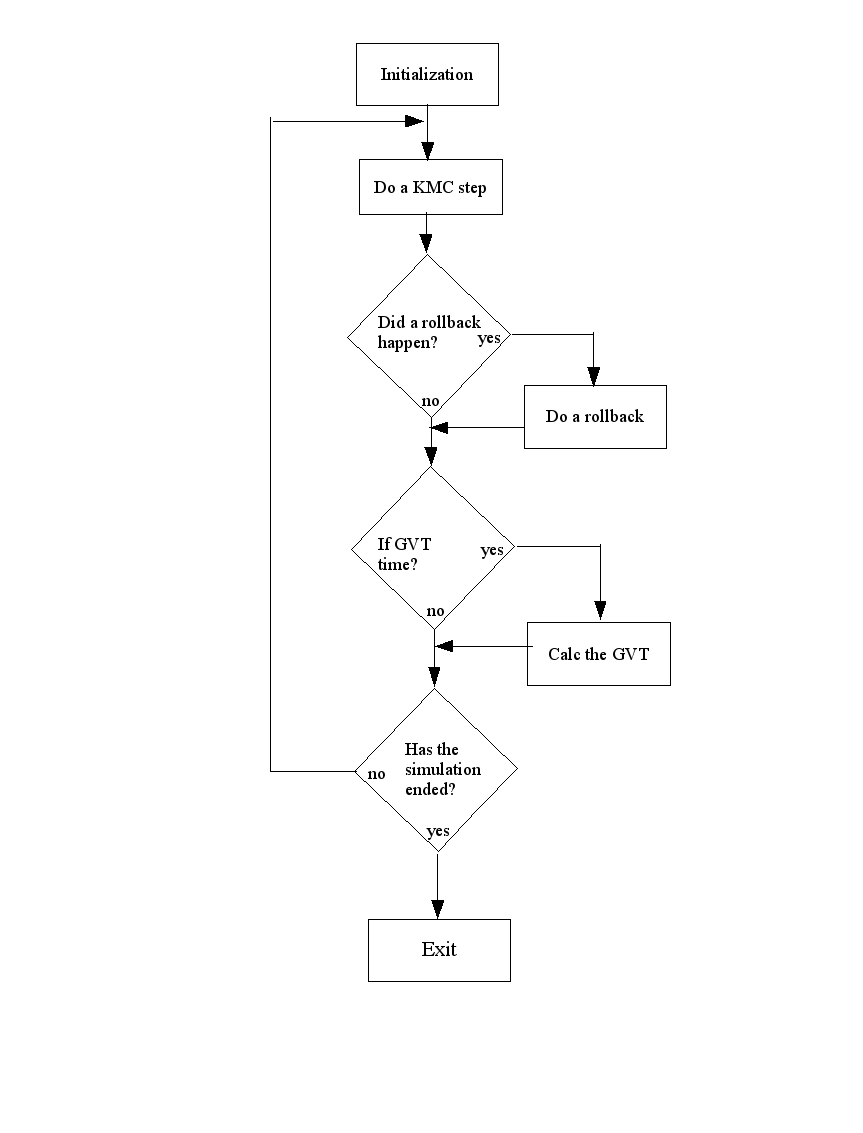
\includegraphics[scale=0.6]{timewarp_flowchart}
\hrule
\caption{Sample KMC Results}
\label{figure:Class Schema}
\end{figure}

The mechanics of the KMC algorithm have already been described in Section \ref{section:Thin Film Growth}.  Since the goal of this project was to delve into the underlying mechanics of the algorithm, of which the KMC was an appropriate problem, the code needed to be written in such a way that it was both flexible and robust.  To facilitate this it was determined that the C++ language would be up to the job.  It was also determined that any of the KMC parts should be as self-contained as possible, which like the re-implementation of SR, was in the form of a Lattice class.  The Lattice class was supported by various layers \ref{figure:Class Schema} of abstraction that removed as much of the implementation dependence as possible.

\section{Implementation}

The actual code base for this implementation of the TW: KMC algorithm is split into an number of files, both C++ source and header files, which contain a number of classes that do nearly all the work.  A text dump of the source files are available in Appendix \ref{ch:Time Warp Code}.

\subsection{Lattice Class}

This sub-section refers to the following appendix sections: \ref{code:tw/lattice.h}, \ref{code:tw/lattice.cpp}, \ref{code:tw/latconst.h}, \ref{code:tw/latprim.h}, \ref{code:tw/rewindlist.h}, \ref{code:tw/randgen.h}, \ref{code:tw/event.h}.

The core of the TW: KMC implementation is a Lattice class.  The design of this class was twofold:  1) To improve on the previous Lattice class as implemented in the new SR code (Appendix \ref{ch:Synchronos Relaxiation Code}) and 2) To build in a new way of handling events that improves the storage and computational efficiency of error correction.

Before the Lattice class proper can be addressed, one must understand the breakdown of the various parts.  In the file \texttt{latprim.h} (Appendix \ref{code:tw/latprim.h}) are the primitive data structures that make up the most atomic parts of an event.  In the file \texttt{event.h} (Appendix \ref{code:tw/event.h}) is the definition of the Event class.  The file \texttt{latconst.h} (Appendix \ref{code:tw/latconst.h}) contains all of the various lattice constants, such as deposition rate and lattice size.  The two support classes, a RewindList abstract data structure (Appendix \ref{code:tw/rewindlist.h}) and a rewindable random number generator (Appendix \ref{code:tw/randgen.h}), are contained in separate files.  The Lattice class is contained in the files \texttt{lattice.h} and \texttt{lattice.cpp} (Appendix \ref{code:tw/lattice.h} and Appendix \ref{code:tw/lattice.cpp}, respectively).

The core of the Lattice class is the event processing.  In previous algorithms, as events are generated they're processed immediately.  Remote events are stored in a buffer and exchanged during a sync.  The same holds true in this implementation, but it is done in a more object-orientated way, where the event becomes an object, and the object is worked upon.

The first that that must be done is determine the locality of the event that must be processed.  Since we're going to be doing error correction using remote events, we must make sure to process events from the remote queue in the correct order.  To do this, we calculate the time of the next local event and compare that value with the earliest event in the remote event queue.  The lowest event is processed.  If it is a local event, we create the event.  For remote events we grab the event out of the queue.

Once we have the event, we proceed to the next step.  This step is to commit the event to the lattice.  At this stage we don't care if it's a remote event or not, and we perform the action, wither deposition or diffusion,  After the event is committed we push it onto a stack of events processed.

Remote events are passed to the communication class, MPIWrapper, during this step as well.  This is a pretty abstract process from the Lattices point-of-view, as all the Lattice needs to know is which boundary the Event occurs on, and what the event is.  The wrapper layer (in this case \texttt{MPIWrapper}) can then translate the passed data and send the event.  The details of this operation in the \texttt{MPIWrapper} layer is covered in Sub-Section \ref{subsection:MPIWrapper Class}.

The Lattice class also needs to check for new remote events.  Currently this is done periodically in the main function, after one event is processed.  This is important, since we must gather the remote events to correct any error we may have made, and to have the events on hand so we don't make an error in the future.  Some though should be put into how often we poll the queue for new remote events.  More often then not, polling once a cycle, we're not going to have any remote events.  However, if we make the polling interval too long, the chances for errors to occur goes up drastically, which means more rollbacks.

The function that polls for remote events is responsible for detecting errors in the simulation as well.  When it finds an error, it will trigger a rollback.  The rollback function takes a single parameter which is the time at which the error occurs.  The rollback function loops through the event stack and compares the top of the stack with the passed timestamp, stopping when the top of the event stack is less-than the passed timestamp.  Each cycle of the loop, if we're not going to halt, the top event is poped off and the event is rolled back on the lattice.  If the event is a remote event, it's stored in the remote event queue, otherwise the event will be discarded.  Sadly, this means that we must send anti-messages for any event that was sent as a boundary event.  Normally this would not be an issue, as the TW algorithm would use lazy evaluation in sending anti-messages, only sending anti-messages for those events that would never happen again.  However, this will be a rare, if not impossible situation, as any KMC event influences the rates for future events, and therefore the probability of that event happening in the same way again.  Since we are almost guaranteed to not repeat the event, we might as well cancel all of the sent events with their anti-message, so we don't need to incur the overhead of lazy evaluation.

The Lattice class would be nearly useless without data output.  There are a variety of ways that one can get data from the Lattice class, including dumps of the height map in both text and as a PNG file.  Also the Lattice and dump it's current monomer list and a collection of various counts and statistics that describe the simulation to that point.  Most of these functions take a output stream as a parameter, with one taking the file name that should be created.

\subsection{MPIWrapper Class} \label{subsection:MPIWrapper Class}
This sub-section refers to the following appendix sections: \ref{code:tw/mpiwrapper.h}, \ref{code:tw/mpiwrapper.cpp}.

The MPIWrapper class is divided into two files, the definition file \texttt{mpiwrapper.h} (Appendix \ref{code:tw/mpiwrapper.h}) and the implementation file \texttt{mpiwrapper.cpp} (Appendix \ref{code:tw/mpiwrapper.cpp}).  Included in these files are any helper structures, such as \texttt{message}.  As the name implies, this class is a wrapper for all of the MPI related calls the program must make.

MPIWrapper provides a number of interfaces for doing various helpful things with MPI.  Included are calls to do global scatter-gather operations and do barrier calls.  The most important interface provided is the sending of events between processes.

The event passing interface is very abstract, compared with previous implementations.  In the original SR code, the MPI calls were performed directly, so the lattice functions needed to know the particulars of the MPI calls and such.  With the MPIWrapper, the Lattice class only needs to pass the event as an Event class pointer and the direction (or boundary) direction as an enumerated integer.  The MPIWrapper call transforms the object as passed into a data structure (type \texttt{message}) which it then can send to the corresponding node.  To mark the type of message, either an event message or anti-message, the tag property of the send call is used.

It should be noted that the send call used in this operation is \texttt{MPI\_Bsend()}, which buffers the message in a local buffer (for this project a 10MB buffer), and only sends the message when the receiving node is ready to receive.  This allows for a asynchronous send, with a blocking receive.

Since the Lattice class must also gather remote events, there is also an interface that returns a list of events as they were received.  There is the possibility that the wrapper could stall out program execution if there are many, many events waiting to be received.  However, this would require a enormous number of events, and in such a situation the current communication model would not be ideal.

The interfaces for sending and receiving anti-messages are the same as the ones provided for normal messages.  The only difference between the function is the tag passed to the MPI calls within.

Also exposed are a suite of function that perform a \texttt{MPI\_Allreduce()}, each function uses a different data type, and takes a data value and a MPI operator as parameters.  This is useful for collecting global statistics and performing the GVT calculation.

Lastly, the MPIWrapper exposes a method to output statistics about it's communications, such as counts of events sent and received and pertinent data about the cluster itself such as number of nodes and who are the neighboring nodes.

\subsection{Main Function and GVT}

This sub-section refers to the following appendix sections: \ref{code:tw/main.cpp}.

The main function of the project is contained in the file \texttt{main.cpp} (Appendix \ref{code:tw/main.cpp}).  Laid out in the main function is the highest level of abstraction in the code, along with the GVT calculation and the calculation of the stopping condition, which is currently the coverage of the lattice.

The level of abstraction in \texttt{main()} is meant to insulate the top level code from the actual processes underneath.  The program is essentially constructed of a main loop that calls a function to process the next event, and then receive and processes any remote events.  Also, at periodic intervals it performs a GVT calculation.  Currently this does nothing as the garbage collection has not been implemented.  The \texttt{main()} function is responsible for outputting the data in various forms along with logging the progress of the simulation for debugging purposes.

The GVT calculation is an all reduce operation that finds the minimum LVT of all the TW objects in the simulation.  This value is set as the GVT.  No event will ever come before this time, so we can effectively delete any data up to that point.  However, this is not done right now.  GVT also makes a decent exit condition for the simulation, is we need not compare the results against previous implementations.

To compare the simulation results against other implementations we need to find the global coverage of the simulation, which requires a second all reduce operation, this time to sum the number of depositions and therefore the number of monomers in the simulation.  To find the coverage we divide the number of monomers by the total surface area of the lattice.  We exit when that value grows greater then 1.0 (100\%).

\section{Issues}

A variety of problems were encountered while implementing the TW algorithm previously described.  Most have been solved, many being bugs with the underlying communication system doing things that more then likely were not intended by the authors.  However, at the time of writing, there has been a bug that shakes the very root of the problem.  Work has stalled out until this bug can be over come.

The bug in question deals with the validity of results obtained at the completion of the simulation.  The results are not consistent from one simulation to the next, which indicates a problem with the rigorous nature of the algorithm.  Normally, the simulation should always, \textit{always}, produce the same results for a given input, baring major hardware failure or a bug (such as the Pentium Floating Point bug) in the actual system hardware.  However, this bug is not a hardware bug, but rather a software bug of the systemic nature.

There could be a variety of causes for such a bug, including a logic error in the error-correction mechanism (rollback) to a race condition.  So far, only a few ideas have been floated, mostly dealing with a race condition between processes to get the first event.  This race condition would then influence the results of the simulation enough to produce drastic results to the final output, as is the nature of the KMC algorithm, one event precipitate further events of random nature.  Logically, however, there are only a few conditions that such a race condition could cause, as there is a limited number of "first events", to start the ensuing chain leading up to the final result.  Suppose that there are $n$ processes, each operating independently of each other.  In the case that thread \#1 were to generate the first event, we would see one result, if the rest of the simulation were truly rigorous.  The same for thread \#2 generating the first event.  It follows that for $n$ processes, we get $n$ results.  This is not observed.

Even if there is not a race condition currently, it may be adding to the problem of debugging the actual cause of the differing results.  A sort of error on-top of an underlying error.  One thing that this implementation discards is the idea of a circular lattice, which is present in the original and rewritten SR algorithms.  The author did not think of the implications of this decision, namely events that happen on the two boundaries that have no neighbors.  In the current TW implementation these messages are just discarded in the wrapper layer.  However, they should be "wrapped around".  This would cause the simulation to disregard the race condition, as it does not matter which process sends or receives the first message since all messages are handled.  The only difference between runs should be the order of the lattices, where the results will be transposed over some number between $0$ and $n-1$ offset from a null state, as the lattice is now a ring, rather then a bar.

It would be more probable that the error occurs during the error-correction sequence.  A logic error in this section of code could precipitate a chain of errors which would end up drastically changing the results.  However, this is a difficult thing to debug, not only because of limitations in the work environment, but because there are many, many events exchanged for a given time period, and it is difficult to sift through them all and make sure all of the events were handled.  This is the next task to tackle and should take a good long time to complete.  Not only will further code need to be written to facilitate this debugging, but then the code will need to be corrected, which in the extreme possibility could necessitate a total rewrite of the error-correction code.  However, this is in the extreme case that it's totally wrong, which isn't very likely.  An educated guess would be that the conditions on the while loops that control the correction are wrong.

It should be noted that both of these conjectures about the possible cause of the current major bug are just that, pure speculation.  Lots of time has been spent on this algorithm, so they are educated guesses, but the root cause could turn out to be something entirely different from the ideas laid out here.  However, once this bug is resolved, there is a good chance that the algorithm is correct and hard performance results can be gathered and future work can take place.
\mychapter{Future Work}

\section{Synchronous Relaxation}

We feel that there is little work left to do on the SR algorithm.  The promise of our work is in the potential improvements that could be made with the Time Warp algorithm.  However, should Time Warp fail, this would be the most promising path for further research, so any work should not be scrapped, but rather shelved until a later date.

\section{Time Warp}

\subsection{Debugging and Validation}
This is by far the first and most important thing that will need to be done to this algorithm.  Only once this step is completed can any future work proceed.  To do this first the difference in results between runs must be identified and suppressed or eliminated.  Secondly, the validity of the results should be sought.  This step could prove to be difficult, as the original SR algorithm should always produce different results then the TW algorithm.  Because of this, the validity of results will nearly always been in question, and should be studied with veracity until we are certain.  Time to complete: 10-30 hours.

\subsection{Garbage Collection and Memory Management}
Right now, there is no garbage collection implemented in the TW algorithm.  Since this algorithm is very memory intensive, garbage collection would be a good thing.  To do this we would need to call a routine every time the GVT is calculated that will delete all of the events that occur before the GVT.  This will free memory for the next GVT cycle.  Also, if user-space memory management was implemented, we could reuse the memory to keep from reallocating the same chunks thus providing more speed to the algorithm. Time to complete: 10-20 hours.

\subsection{Logical Processes}
One of the primary goals of the TW algorithm was to add more processor independence to the KMC algorithm.  Thus far, the algorithm has seemed to do this, and now the limiting factor is the problem size and physical hardware restrictions such as memory.  However, we can go a step farther and apply a concept called logical processes to the algorithm to produce a truly processor independent implementation.

Logical processes essentially encapsulate a single KMC process.  Currently, each node on a cluster will execute one process.  With logical processes each node will execute tens, hundreds, or thousands of similar processes in such a way as to simulate the running of just one process on a single node.  To accomplish this, there must be a middle-ware layer between the program and the message passing interface.  This middle layer handles both external MPI communication with other nodes, and interval node communication between logical processes on the same node.  The goal of this middle layer is to make it as transparent as possible, the calling thread should not know if the process that will be receiving the message is local logical process or a remote (on another node) logical thread.

To complete this task a variety of things will need to be completed.  First a formal study of the middle-ware layer as exposed by the BGTW simulation library should be undertake to judge the usefulness of this established code base.  Secondly, any changed that will need to be made to the algorithm should be performed and then the simulation revalidated to ensure that the algorithm is still correct.  Thirdly, the middle-ware layer should be integrated into the existing algorithm and validated.  This last step will produce the final logical process version of the TW algorithm. Time to complete: 20-50 hours.

\section{General}

\subsection{2D Decomposition}
The current algorithms work with at 1D decomposition or strip lattice where there is at most only two neighboring lattices any given lattice.  This is limiting however in total scale of problem, as to increase the total area we must increase the height and width of the lattice.  Eventually the number of boundary events exchanged over a single boundary will slow the overall execution down.  At this point it will be beneficial to split a single sub-lattice into a 2D map of adjoining lattices.  We can then scale the problem up further till we reach the same limiting factor as before.  Time to complete: 20-40 hours.


\appendix

\mychapter{Synchronos Relaxiation Code}

% MAIN SOURCE FILE
\section{main.cpp}
\begin{code}{main.cpp}{sr/main.cpp}
{\ttfamily \raggedright \footnotesize
\#include\ "{}lattice.h"{}

MPIWrapper\ mpi;
int\ main(int\ argc,char\ *\ argv[])
\{
\ \ int\ i,ctr,myid=0;
\ \ int\ totaldep;

\ \ mpi.init(\&argc,\&argv);

\ \ myid=mpi.getRank();
\ \ Lattice\ newlatt;
\ \ float\ cov,COV=1,T=0.001;
\ \ newlatt.nbhr[left]=LEFT(myid);
\ \ newlatt.nbhr[right]=RIGHT(myid);

\ \ while(cov<{}=COV)
\ \ \{
\ \ \textsl{/**/}
\ \ newlatt.time=0;
\ \ newlatt.nevent=0;
\ \ newlatt.randgen();
\ \ newlatt.iran=0;
\ \ newlatt.saveconfig();

\ \ newlatt.bdycountrec[left]=0;
\ \ newlatt.bdycountrec[right]=0;


\ \ while(newlatt.time<{}T\ )
\ \ \ \ \{
\ \ \ \ \ \ if(newlatt.time<{}=T)
\ \ \ \ \{
\ \ \ \ newlatt.doKMC();
\ \ \ \ newlatt.calctime();
\ \ \ \ \}
\ \ \ \ \ \ \ \
\ \ \ \ \}
\ \ \ \ \ \ \
\ \ newlatt.savebdylist();
\ \ \ \ \ \
\ \ sendmsgs(\&newlatt);
\ \ synch(\&newlatt);
\ \ mpi.allReduce(\&totaldep,\&newlatt.ndep,1,MPI\underline\ FLOAT,MPI\underline\ SUM);
\ \ cov=(float)\ totaldep/(float)(2*size*size);
\ \ cout<{}<{}"{}cov="{}<{}<{}cov<{}<{}endl;
\ \ ctr++;
\ \ \}

\ \ cout<{}<{}"{}latone*******************"{}<{}<{}endl;
\ \ newlatt.p();

\ \ mpi.shutdown();

\ \ return\ 0;
\}


 }
\normalfont\normalsize


\end{code}

% LATTICE SOURCE FILES
\section{lattice.h}
\begin{code}{lattice.h}{sr/lattice.h}
{\ttfamily \raggedright \small
\#include\ <{}vector>{}\\
using\ std::vector;\\
\ \\
\#include\ <{}queue>{}\\
using\ std::priority\underline\ queue;\\
\ \\
\#include\ <{}stack>{}\\
using\ std::stack;\\
\ \\
\#include\ <{}iomanip>{}\\
using\ std::setw;\\
using\ std::hex;\\
using\ std::dec;\\
using\ std::setprecision;\\
\ \\
\#include\ <{}fstream>{}\\
using\ std::fstream;\\
\ \\
\#include\ <{}string>{}\\
using\ std::string;\\
\ \\
\#include\ <{}png.h>{}\\
\ \\
\#include\ "{}exception.h"{}\\
\#include\ "{}latprim.h"{}\\
\#include\ "{}latconst.h"{}\\
\#include\ "{}event.h"{}\\
\#include\ "{}randgen.h"{}\\
\#include\ "{}rewindlist.h"{}\\
\#include\ "{}mpiwrapper.h"{}\\
\ \\
\#ifndef LATTICE\underline\ H\\
\#define LATTICE\underline\ H\\
\ \\
\#define GET\underline\ DIR(a)\ ((a\ <{}\ LEFT\underline\ X\underline\ BOUNDRY)\ ?\ LEFT\ :\ RIGHT)\\
\ \\
class\ Lattice\ \{\\
public:\\
\ \ Lattice();\\
\ \ \textasciitilde Lattice();\\
\ \\
\ \ void\ cleanup(fstream\&);\\
\ \\
\ \ bool\ doNextEvent();\\
\ \\
\ \ double\ getLocalTime()\ \{\\
\ \ \ \ return(localTime);\\
\ \ \}\\
\ \\
\ \ bool\ setMinGlobalTime(double\ mGT)\ \{\\
\ \ \ \ minGlobalTime\ =\ mGT;\\
\ \ \ \ return(true);\\
\ \ \}\\
\ \\
\ \ double\ getMinGlobalTime()\ \{\\
\ \ \ \ return(minGlobalTime);\\
\ \ \}\\
\ \\
\ \ bool\ negoitateEvents(fstream\&);\\
\ \\
\ \ \textsl{//\ DEBUG\ FUNCTIONS}\\
\ \ void\ printLatticeHeight(fstream\&\ file)\ \{\\
\ \ \ \ for(int\ i=0;\ i\ <{}\ DIM\underline\ X\ +\ GHOST\ +\ GHOST;\ ++i)\ \{\\
\ \ \ \ \ \ for(int\ j=0;\ j\ <{}\ DIM\underline\ Y;\ ++j)\ \{\\
\ \ \ \ \ \ \ \ file\ <{}<{}\ lattice[i][j].h\ <{}<{}\ "{}\ "{};\\
\ \ \ \ \ \ \}\\
\ \ \ \ \ \ file\ <{}<{}\ endl;\\
\ \ \ \ \}\\
\ \ \ \ file\ <{}<{}\ "{}-{}-{}-{}-{}-{}-{}-{}-{}-{}-{}-{}-{}-{}-{}-{}-{}-{}-{}-{}-{}-{}-{}-{}-{}-{}-{}-{}-{}-{}-{}-{}-{}-{}-{}-{}-{}-{}-{}-{}-{}-{}-{}-{}-{}-{}-{}-{}-{}"{}\ <{}<{}\ endl\ <{}<{}\ endl;\\
\ \ \ \ file.flush();\\
\ \ \}\\
\ \\
\ \ void\ printLatticeIndex(fstream\&\ file)\ \{\\
\ \ \ \ for(int\ i=0;\ i\ <{}\ DIM\underline\ X\ +\ GHOST\ +\ GHOST;\ ++i)\ \{\\
\ \ \ \ \ \ for(int\ j=0;\ j\ <{}\ DIM\underline\ Y;\ ++j)\ \{\\
\ \ \ \ \ \ \ \ if(lattice[i][j].listIndex\ >{}=\ 0)\\
\ \ \ \ \ \ \ \ \ \ file\ <{}<{}\ setw(4)\ <{}<{}\ lattice[i][j].listIndex;\\
\ \ \ \ \ \ \ \ else\\
\ \ \ \ \ \ \ \ \ \ file\ <{}<{}\ setw(4)\ <{}<{}\ "{}x"{};\\
\ \ \ \ \ \ \ \ file\ <{}<{}\ "{}\ "{};\\
\ \ \ \ \ \ \}\\
\ \ \ \ \ \ file\ <{}<{}\ endl;\\
\ \ \ \ \}\\
\ \ \ \ file\ <{}<{}\ "{}-{}-{}-{}-{}-{}-{}-{}-{}-{}-{}-{}-{}-{}-{}-{}-{}-{}-{}-{}-{}-{}-{}-{}-{}-{}-{}-{}-{}-{}-{}-{}-{}-{}-{}-{}-{}-{}-{}-{}-{}-{}-{}-{}-{}-{}-{}-{}-{}"{}\ <{}<{}\ endl\ <{}<{}\ endl;\\
\ \ \ \ file.flush();\\
\ \ \}\\
\ \\
\ \ void\ printMonomerList(fstream\&\ file)\ \{\\
\ \ \ \ file\ <{}<{}\ "{}monomerList["{}\ <{}<{}\ monomerList.size()\ <{}<{}\ "{}]\ at\ time="{}\ <{}<{}\ localTime\ <{}<{}\ endl;\\
\ \ \ \ for(int\ i=0;\ i\ <{}\ monomerList.size();\ ++i)\ \{\\
\ \ \ \ \ \ site$\ast$\ s\ =\ monomerList[i];\\
\ \ \ \ \ \ file\ <{}<{}\ i\ <{}<{}\ "{}:\ ("{}\ <{}<{}\ s-{}>{}p.x\ <{}<{}\ "{},"{}\ <{}<{}\ s-{}>{}p.y\ <{}<{}\ "{})\ h="{}\ <{}<{}\ s-{}>{}h\ <{}<{}\ "{}\ listIndex="{}\ <{}<{}\ s-{}>{}listIndex\ <{}<{}\ "{}\ "{}\ <{}<{}\ hex\ <{}<{}\ s\ <{}<{}\ dec\ <{}<{}\ endl;\\
\ \ \ \ \}\\
\ \ \ \ file\ <{}<{}\ "{}-{}-{}-{}-{}-{}-{}-{}-{}-{}-{}-{}-{}-{}-{}-{}-{}-{}-{}-{}-{}-{}-{}-{}-{}-{}-{}-{}-{}-{}-{}-{}-{}-{}-{}-{}-{}-{}-{}-{}-{}-{}-{}-{}-{}-{}-{}-{}-{}"{}\ <{}<{}\ endl\ <{}<{}\ endl;\\
\ \ \ \ file.flush();\\
\ \ \}\\
\ \\
\ \ void\ printStats(fstream\&\ file)\ \{\\
\ \ \ \ file\ <{}<{}\ setprecision(10)\ <{}<{}\ endl;\\
\ \ \ \ file\ <{}<{}\ "{}COLLECTED\ STATISTICS"{}\ <{}<{}\ endl;\\
\ \ \ \ file\ <{}<{}\ "{}-{}-{}-{}-{}-{}-{}-{}-{}-{}-{}-{}-{}-{}-{}-{}-{}-{}-{}-{}-{}-{}-{}"{}\ <{}<{}\ endl;\\
\ \ \ \ file\ <{}<{}\ "{}Convergence\ =\ "{}\ <{}<{}\ getConvergence()\ <{}<{}\ endl;\\
\ \ \ \ file\ <{}<{}\ "{}Total\ Event\ Count\ =\ "{}\ <{}<{}\ countEvents\ <{}<{}\ endl;\\
\ \ \ \ file\ <{}<{}\ "{}Total\ Diffusion\ Events\ =\ "{}\ <{}<{}\ countDiffusion\ <{}<{}\ endl;\\
\ \ \ \ file\ <{}<{}\ "{}Total\ Deposition\ Events\ =\ "{}\ <{}<{}\ (countEvents\ -{}\ countDiffusion)\ <{}<{}\ endl;\\
\ \ \ \ file\ <{}<{}\ "{}Total\ Boundry\ Events\ =\ "{}\ <{}<{}\ countBoundry\ <{}<{}\ endl;\\
\ \ \ \ file\ <{}<{}\ "{}Total\ Number\ Remote\ Events\ =\ "{}\ <{}<{}\ countRemote\ <{}<{}\ endl;\\
\ \ \ \ file\ <{}<{}\ "{}Total\ Rollbacks\ Performed\ =\ "{}\ <{}<{}\ countRollback\ <{}<{}\ endl;\\
\ \ \ \ file\ <{}<{}\ "{}Monomer\ List\ Size\ =\ "{}\ <{}<{}\ monomerList.size()\ <{}<{}\ endl;\\
\ \ \ \ file\ <{}<{}\ "{}Local\ Time\ =\ "{}\ <{}<{}\ localTime\ <{}<{}\ endl;\\
\ \ \ \ file\ <{}<{}\ "{}Min\ Global\ Time\ =\ "{}\ <{}<{}\ minGlobalTime\ <{}<{}\ endl;\\
\ \ \ \ file\ <{}<{}\ "{}Size\ =\ "{}\ <{}<{}\ SIZE\ <{}<{}\ "{}\ DIM\underline\ X\ =\ "{}\ <{}<{}\ DIM\underline\ X\ <{}<{}\ "{}\ DIM\underline\ Y\ =\ "{}\ <{}<{}\ DIM\underline\ Y\ <{}<{}\ endl;\\
\ \ \ \ file\ <{}<{}\ "{}-{}-{}-{}-{}-{}-{}-{}-{}-{}-{}-{}-{}-{}-{}-{}-{}-{}-{}-{}-{}-{}-{}-{}-{}-{}-{}-{}-{}-{}-{}-{}-{}-{}-{}-{}-{}-{}-{}-{}-{}-{}-{}-{}-{}-{}-{}-{}-{}"{}\ <{}<{}\ endl\ <{}<{}\ endl;\\
\ \ \ \ file.flush();\\
\ \ \}\\
\ \\
\ \ int\ getEventCount()\ \{\ return(countEvents\ -{}\ countDiffusion);\ \}\\
\ \\
\ \ bool\ createHeightMap(string\ filename);\\
\ \\
\ \ MPIWrapper\ mpi;\ \ \textsl{//\ I\ can't\ think\ of\ a\ better\ place\ for\ this.}\\
\ \\
\ \ bool\ rollback(const\ double);\\
\ \\
\ \ double\ getConvergence()\ \{\\
\ \ \ \ return((double)(countEvents\ -{}\ countDiffusion)\ /\ (double)(DIM\underline\ X\ $\ast$\ DIM\underline\ Y));\\
\ \ \}\\
\ \\
private:\\
\ \ double\ computeTime();\\
\ \ bool\ deposit();\\
\ \ bool\ diffuse();\\
\ \ bool\ doKMC();\\
\ \ EventType\ getNextEventType();\\
\ \ bool\ commitEvent(Event$\ast$);\\
\ \ site$\ast$\ randomMove(site$\ast$);\\
\ \ bool\ isBoundry(point);\\
\ \ bool\ isBound(site$\ast$);\\
\ \ bool\ clearBonded(site$\ast$,const\ double);\\
\ \ bool\ translateMessages(vector<{}Event$\ast$>{}$\ast$\ ,\ vector<{}message>{}$\ast$);\\
\ \ message$\ast$\ makeMessage(Event$\ast$);\\
\ \ bool\ hasAntiEvent(Event$\ast$);\\
\ \\
\ \ double\ localTime;\ \ \ \ \textsl{//\ the\ time\ local\ to\ the\ lattice}\\
\ \ double\ minGlobalTime;\ \textsl{//\ the\ minimum\ Global\ time\ (point\ of\ no\ return)}\\
\ \\
\ \ RewindList<{}site\ $\ast$>{}\ monomerList;\ \textsl{//\ list\ of\ all\ unbound\ monomers}\\
\ \ \textsl{//site\ lattice[DIM\underline\ X\ +\ GHOST\ +\ GHOST][DIM\underline\ Y];\ \ //\ the\ lattice\ (the\ extra\ two\ are\ the\ ghost\ region)}\\
\ \ site$\ast$$\ast$\ lattice;\\
\ \\
\ \ float\ depositionRate;\ \textsl{//\ the\ deposition\ rate\ of\ monomers}\\
\ \ float\ diffusionRate;\ \ \textsl{//\ the\ diffusion\ rate\ of\ monomers}\\
\ \\
\ \ int\ countDiffusion;\\
\ \ int\ countEvents;\\
\ \ int\ countBoundry;\\
\ \ int\ countRemote;\\
\ \ int\ countRollback;\\
\ \\
\ \ priority\underline\ queue<{}Event$\ast$>{}\ remoteEventList;\ \textsl{//\ list\ of\ all\ the\ remote\ dep/diffusion\ events}\\
\ \ stack<{}Event$\ast$>{}\ eventList;\ \ \ \ \ \ \ \ \ \ \ \ \ \ \ \ \textsl{//\ stack\ of\ all\ events\ to\ rollback\ the\ simulation}\\
\ \ vector<{}Event$\ast$>{}\ antiEvents;\ \ \ \ \ \ \ \ \ \ \ \ \ \ \textsl{//\ list\ of\ anti-{}events\ that\ will\ occur\ in\ the\ future}\\
\ \\
\ \ RandGen\ rng;\ \textsl{//\ random\ number\ generator}\\
\ \\
\ \ point\ movementDir[NUM\underline\ DIR];\ \textsl{//\ array\ of\ movement\ types}\\
\ \ message\ m;\ \textsl{//\ message\ for\ sending\ events}\\
\};\\
\ \\
\#endif\\
\ \\
 }
\normalfont\normalsize


\end{code}

\section{lattice.cpp}
\begin{code}{lattice.cpp}{sr/lattice.cpp}
{\ttfamily \raggedright \footnotesize
\#include\ "{}lattice.h"{}
point\ Lattice::ranmove(site\ mysite)
\{

\ \ \ \ point\ pt;
\ \ \ \ pt.x=0;pt.y=0;

\ \ \ \ \textsl{////cout<{}<{}xdir<{}<{}"{}\ \ "{};\ \ }
\ \ \ \
\ \ \ \ int\ prob=ranlist[iran]*4;\textsl{//rand()\%4;}
\ \ \ \ iran++;
\ \ \ \
\ \ \ \
\ \ \ \ pt.x=mysite.pos.x+mdir[prob].x;
\ \ \ \ pt.y=mysite.pos.y+mdir[prob].y;

\ \ \ \ \textsl{//Allow\ boundary\ movement}
\ \ \ \ \textsl{//No!!!}
\ \ \ \
\ \ \ \ if(pt.x>{}=size+2)\ pt.x-{}=1;
\ \ \ \ if(pt.x<{}0)pt.x+=1;
\ \ \ \
\ \ \ \
\ \ \ \ if(pt.y>{}=size)pt.y-{}=2;
\ \ \ \ if(pt.y<{}0)pt.y+=2;
\ \ \ \
\ \ \ \ return\ pt;
\}

Lattice::Lattice()
\{

\ \ \ \ float\ ratio=0.0;
\ \ \ \ float\ prob;
\ \ \ \ point\ newsite;
\ \ \ \ mcount=0;
\ \ \ \ deprate=1.0f,difrate=1.0e3;
\ \ \ \ ndep=0;
\ \ \ \ nevent=0;
\ \ \ \ time=0;
\ \ \ \ iran=0;
\ \ \ \ subcycle=0;
\ \ \ \ T=0.001;

\ \ \ \ int\ i=0,j=0;
\ \ \ \
\ \ \ \ for\ (i=0;i<{}2;i++)
\ \ \ \ \ \ \ \ bdycount[i]=0;

\ \ \ \ for\ (i=0;i<{}2;i++)
\ \ \ \ \ \ bdycountrec[i]=0;

\ \ \ \ for\ (i=0;i<{}2;i++)
\ \ \ \ \ \ oldbdycountrec[i]=0;

\ \ \ \ for\ (i=0;i<{}size+2;i++)
\ \ \ \ \{
\ \ \ \ for\ (j=0;j<{}size;j++)
\ \ \ \ \ \ \{
\ \ \ \ \ \ \ \ newsite.x=i;
\ \ \ \ \ \ \ \ newsite.y=j;
\ \ \ \ \ \ \ \ location[i][j].pos=newsite;
\ \ \ \ \ \ \ \ location[i][j].h=0;
\ \ \ \ \ \ location[i][j].index=-{}1;
\ \ \ \ \ \ \}
\ \ \ \ \}
\ \ \ \
\ \ \ \
\ \ \ \ \textsl{//generate\ random\ numbers}
\ \ \ \
\ \ \ \ \textsl{//randgen();}
\ \ \ \
\ \ \ \ \textsl{/*
\ \ \ \ generate\ points\ in\ the\ form\ e.g\ (1,-{}1)\ move\ one\ unit\ left\ in\ x\ and\ and\ one\ unit\ up
\ \ \ \ do\ not\ allow\ particle\ to\ remain\ (0,0)
\ \ \ \ */}


\ \ \ \ \textsl{/*Set\ directions*/}



\ \ \ \ mdir[0].y=\ 1;\ \ mdir[0].x=\ 0;
\ \ \ \ mdir[1].y=\ 0;\ \ mdir[1].x=\ 1;
\ \ \ \ mdir[2].y=-{}1;\ \ mdir[2].x=\ 0;
\ \ \ \ mdir[3].y=\ 0;\ \ mdir[3].x=-{}1;
\ \ \ \ mdir[4].y=\ 1;\ \ mdir[4].x=\ 1;
\ \ \ \ mdir[5].y=\ 1;\ \ mdir[5].x=-{}1;
\ \ \ \ mdir[6].y=-{}1;\ \ mdir[6].x=\ 1;
\ \ \ \ mdir[7].y=-{}1;\ \ mdir[7].x=-{}1;

\}
void\ Lattice::calctime()
\{
\ \ float\ \ \ monomer=(float)mcount,
\ \ \ \ Drate=difrate*monomer*0.25f,
\ \ \ \ N=(float)latsize,dt,prob,
\ \ \ \ totaldep=deprate*N;
\ \ \
\ \ prob\ =\ ranlist[iran];
\ \ \ \ \ \ \ \ iran++;
\ \ dt=-{}log(prob)/(Drate+totaldep);
\ \ time+=dt;
\}
Lattice::\textasciitilde Lattice()
\{

\}

int\ Lattice::getbonds(site\ mysite,point\ *\ bondpt)
\{
int\ ctr=0,i=0;
point\ pt;
pt=mysite.pos;
for(;i<{}dir;i++)
\{
\ \ \ pt.x+=mdir[i].x;
\ \ \ pt.y+=mdir[i].y;
\ \ \ if((pt.x<{}0)
\ \ \ \ \ \ ||(pt.x>{}=size+2)
\ \ \ \ \ \ ||(pt.y<{}0)
\ \ \ \ \ \ ||(pt.y>{}=size))
\ \ \{
\
\ \ \}
\ \ else
\ \ \{
\ \ \ \ \ if(location[pt.x][pt.y].h>{}=mysite.h)
\ \ \ \ \ \{
\ \ \ \ \ \ \ bondpt[ctr]=pt;
\ \ \ \ ctr++;
\ \ \ \ \ \}
\ \ \ \}
\ \ \ pt=mysite.pos;
\}
return\ ctr;
\}

int\ Lattice::getnbhrs(site\ mysite,point\ *\ bondpt)
\{
\ \ \ \ int\ ctr=0,i=0;
\ \ \ \ point\ pt;
\ \ \ \ pt=mysite.pos;
\ \ \ \ for(;i<{}dir;i++)
\ \ \ \ \{
\ \ \ \ pt.x+=mdir[i].x;
\ \ \ \ pt.y+=mdir[i].y;
\ \ \ \ if((pt.x<{}0)
\ \ \ \ \ \ ||(pt.x>{}=size+2)
\ \ \ \ \ \ ||(pt.y<{}0)
\ \ \ \ \ \ ||(pt.y>{}=size))
\ \ \ \ \{
\ \ \ \ \
\ \ \ \ \}
\ \ \ \ else
\ \ \ \ \{
\ \ \ \ \ \ \ \ \ bondpt[ctr]=pt;
\ \ \ \ \ \ ctr++;
\ \ \ \ \ \ \ \
\ \ \ \ \}
\ \ \ \ pt=mysite.pos;
\ \ \ \ \}
\ \ \ \ return\ ctr;
\}

void\ Lattice::deletemonomer(point\ pos)
\{
\ \ point\ lastpt;
\ \ if(mcount>{}1)
\ \ \{
\ \ \ \ lastpt=monomerloc[mcount-{}1];
\ \ \ \ addmonomerchange(diff,lastpt);
\ \ \ \ location[lastpt.x][lastpt.y].index=location[pos.x][pos.y].index;
\ \ \ \ monomerloc[location[pos.x][pos.y].index]=monomerloc[mcount-{}1];
\ \ \ \ location[pos.x][pos.y].index=-{}1;
\ \ \ \ mcount-{}-{};
\ \ \}
\ \ else
\ \ \{
\ \ \ \ location[pos.x][pos.y].index=-{}1;
\ \ \ \ mcount-{}-{};
\ \ \}
\}

bool\ Lattice::neighborIsMonomer(point\ pt,site\ mysite)
\{
\ \ bool\ bMonomer=false;
\ \ \textsl{//if\ index\ is\ not\ -{}1\ and\ same\ height\ as\ my\ location}
\ \ if\ (location[pt.x][pt.y].index!=-{}1\ \&\&\ (location[pt.x][pt.y].h==location[mysite.pos.x][mysite.pos.y].h))
\ \ \ \ \{
\ \ \ \ \ \ bMonomer=true;\ \ \ \
\ \ \ \ \}
\ \ return\ bMonomer;
\}
bool\ Lattice::checkupdatebonds(site\ mysite)
\{
\ \ \textsl{/*
\ \ Possible\ Scenarios
\ \ Deposit
\ \ 1.\ Monomer\ encounters\ no\ cluster\ or\ other\ neighbor\ monomer
\ \ -{}No\ bonds
\ \ 2.\ Monomer\ encounters\ cluster
\ \ -{}bond\ delete\ monomer\ from\ list
\ \ 3.\ Monomer\ encounters\ single\ monomer
\ \ -{}bond.\ delete\ BOTH\ from\ list

\ \ Diffusion
\ \ 1.\ Monomer\ encounters\ no\ cluster\ or\ other\ neighbor\ monomer
\ \ -{}No\ bonds
\ \ 2.\ Monomer\ encounters\ cluster
\ \ -{}bond\ delete\ monomer\ from\ list
\ \ 3.\ Monomer\ encounters\ single\ monomer
\ \ -{}bond.\ delete\ BOTH\ from\ list
\ \ */}
\ \ bool\ bond=false;
\ \ point\ pt,\ bondpt[dir],lastpt;
\ \ int\ i=0,j=0,ctr=0;
\ \ ctr=getbonds(mysite,bondpt);
\ \ if(ctr==0)
\ \ \{
\ \ \textsl{//No\ cluster\ or\ monomer;}
\ \ bond=false;
\ \ \}
\ \ else
\ \ \{
\ \ \textsl{//for\ each\ bond\ recieved}
\ \ bond=true;
\ \ for(;j<{}ctr;j++)
\ \ \ \ \ \ \ \{
\ \ \ \ pt=bondpt[j];
\ \ \ \ \textsl{//if\ monomer\ means\ it\ has\ an\ index}
\ \ \ \ if(neighborIsMonomer(pt,mysite))
\ \ \ \ \ \ \{
\ \ \ \ \ \ \textsl{//delete\ both\ you\ and\ monomer}
\ \ \ \ \ \ \textsl{//delete\ monomer}
\ \ \ \ \ \ deletemonomer(pt);
\ \ \ \ \ \ \}
\ \ \ \ \}
\ \ \ \ \ \ \textsl{//delete\ your\ self\ IF\ you\ are\ a\ monomer}
\ \ \ \ if(mysite.index!=-{}1)
\ \ \ \ \{
\ \ \ \ \textsl{//rearrange\ list\ if\ mcount\ is\ greater\ than\ 1}
\ \ \ \ \ \ deletemonomer(mysite.pos);
\ \ \ \ \}

\ \ \}
\ \ return\ bond;
\}

void\ Lattice::upnbhd(site\ mysite)
\{
\ \ \ \ \ \ \ \ bool\ bond=false;
\ \ point\ pt,\ bondpt[dir],lastpt;
\ \ int\ x,y;
\ \ int\ i=0,j=0,ctr=0;
\ \ ctr=getnbhrs(mysite,bondpt);
\ \ \textsl{//cout<{}<{}"{}getcte="{}<{}<{}ctr<{}<{}endl;}
\ \ \ checksite(mysite);
\ \ \ \ for(i=0;i<{}ctr;i++)
\ \ \ \ \{
\ \ \ \ \ \ \ x=bondpt[i].x;
\ \ \ \ \ \ \ y=bondpt[i].y;
\ \ \ \ \ \ \ checksite(location[x][y]);\textsl{//bond=checkupdatebonds(location[bondpt[i].x][bondpt[i].y]);}
\ \ \ \ \}
\ \ \ \ \ \ \ if(mysite.h<{}=0\ \&\&\ mysite.index!=-{}1)
\ \ \ \ \ \ \ \ \ \{
\ \ \ \ \ \ deletemonomer(mysite.pos);
\ \ \ \}

\}
void\ Lattice::checksite(site\ mysite)
\{
\ \ bool\ bond=false;
\ \ bond=checkupdatebonds(location[mysite.pos.x][mysite.pos.y]);\ \ \
\ \ \ \ if(bond==false)
\ \ \ \ \{
\ \ \ \ \ \ \ \ if((location[mysite.pos.x][mysite.pos.y].index==-{}1)\ \&\&(location[mysite.pos.x][mysite.pos.y].h>{}0))
\ \ \ \ \ \ \ \ \ \{
\ \ \ \ \ \ \ \ \ \ \ \ location[mysite.pos.x][mysite.pos.y].index=mcount;
\ \ \ \ \ \ \ \ \ \ \ \ monomerloc[mcount]=location[mysite.pos.x][mysite.pos.y].pos;
\ \ \ \ \ \ \ \ \ \ \ \ mcount++;
\ \ \ \ \ \ \ addmonomerchange(0,mysite.pos);
\ \ \ \ \ \ \ \ \ \}
\ \ \ \ \}
\}
void\ Lattice::addmonomerchange(int\ tag,int\ lastpoint)
\{
\ \ change[changecount].time=time;
\ \ if(tag==0)
\ \ \{
\ \ \ \ myevents[eventcount].oldval=monomerloc[count];
\ \ \ \ change[changecount].newsite=mcount;
\ \ \ \ change[changecount].newval=monomerloc[mcount];
\ \ \ \ change[changecount].tag=0;
\ \ \ \ changecount++;
\ \ \}
\ \ else
\ \ \{
\ \ \ \ change[changecount].oldsite=lastpoint;
\ \ \ \ change[changecount].oldval=monomerloc[lastpoint];
\ \ \ \ change[changecount].newsite=count-{}1;
\ \ \ \ change[changecount].newval=monomerloc[count-{}1];
\ \ \ \ change[changecount].tag=1;
\ \ \ \ changecount++;
\ \ \}

\}
void\ Lattice::restorelist(float\ Ctime)
\{
\ \ int\ oldloc,newloc,tag;
\ \ site\ oldval,newval;
\ \ int\ j=changecount-{}1;
\ \ while(change[j].time>{}Ctime)
\ \ \{
\ \ oldloc=change[j].oldsite;
\ \ newloc=change[j].newsite;
\ \ oldval=change[j].oldval;
\ \ newval=change[j].newval;
\ \ tag=change[j].tag;
\ \ if(tag==1)
\ \ \ \ \ \ \ \{
\ \ \ \ monomerloc[newloc]=newval;
\ \ \ \ \ \ \ monomerloc[oldloc]=oldval;
\ \ \ \ mcount++;
\ \ \ \ \}
\ \ else
\ \ \ \ \{
\ \ \ \ monomerloc[newloc]=oldval;
\ \ \ \ mcount-{}-{};
\ \ \ \ \}
\ \ \ \ j-{}-{};
\ \ \}
\}
void\ Lattice::saveconfig()
\{
\ \ int\ j;
\ \ for\ (j=0;j<{}mcount;j++)
\ \ \{
\ \ \ \ \ \ oldlist.monomerloc[j]=monomerloc[j];
\ \ \}
\ \ \
\ \ oldlist.mcount=mcount;
\ \ oldlist.ndep=ndep;
\}

void\ Lattice::restorelist()
\{
\ \ int\ j;
\ \ for\ (j=0;j<{}oldlist.mcount;j++)
\ \ \{
\ \ \ \ monomerloc[j]=oldlist.monomerloc[j];
\ \ \}
\
\ \ mcount=oldlist.mcount;
\ \ ndep=oldlist.ndep;
\}

void\ Lattice::restoreLattice()
\{
\ \ \ undoevent();
\ \ \ restorelist();
\ \ \ int\ i,j;
\ \ \ int\ x,y;
\ \ \ \textsl{/**clear\ lattice**/}
\ \ \ for(i=0;i<{}size+2;i++)
\ \ \ \{
\ \ \ \ \ for(j=0;j<{}size;j++)
\ \ \ \ \ \{
\ \ \ \ \ \ \ \ location[i][j].index=-{}1;
\ \ \ \ \ \}
\ \ \ \}
\ \
\ \ \ \textsl{/** restore\ indexes*/}
\ \ \ for(i=0;i<{}mcount;i++)
\ \ \ \{
\ \ \ \ \ x=monomerloc[i].x;
\ \ \ \ \ y=monomerloc[i].y;
\ \ \ \ \ location[x][y].index=i;
\ \ \ \}
\}

void\ Lattice::restoreLattice(float\ Ctime)
\{
\ \ undoevent(Ctime);
\ \ restorelist(Ctime);
\ \ int\ i,j;
\ \ int\ x,y;
\ \ \textsl{/**clear\ lattice**/}
\ \ for(i=0;i<{}size+2;i++)
\ \ \{
\ \ \ \ for(j=0;j<{}size;j++)
\ \ \ \ \{
\ \ \ \ \ \ location[i][j].index=-{}1;
\ \ \ \ \}
\ \ \}
\ \ \ \
\ \ \textsl{/** restore\ indexes*/}
\ \ for(i=0;i<{}mcount;i++)
\ \ \{
\ \ \ \ x=monomerloc[i].x;
\ \ \ \ y=monomerloc[i].y;
\ \ \ \ location[x][y].index=i;
\ \ \}
\}

void\ Lattice::addbdyevent(site\ oldsite,site\ newsite,float,int\ tag)
\{
\ \ //add\ boundary\ events\ to\ list
\ \ \ \ int\ bdyrightcount=bdycount[right],bdyleftcount=bdycount[left];
\ \ //erase\ pointers
\ \ \ \ oldsite.index=-{}1;newsite.index=-{}1;
\ \ if((oldsite.pos.x>{}=size)\ ||\ (newsite.pos.x>{}=size))
\ \ \{
\ \ \ \ if(oldsite.pos.x==size)
\ \ \ \ \{
\ \ \ \ \ \ oldsite.pos.x=0;
\ \ \ \ \}
\ \ \ \
\ \ \ \ if(oldsite.pos.x==size+1)
\ \ \ \ \{
\ \ \ \ \ \ oldsite.pos.x=1;
\ \ \ \ \}
\ \ \ \
\ \ \ \ if(newsite.pos.x==size)
\ \ \ \ \{
\ \ \ \ \ \ newsite.pos.x=0;
\ \ \ \ \}
\ \ \ \
\ \ \ \ if(newsite.pos.x==size+1)
\ \ \ \ \{
\ \ \ \ \ \ newsite.pos.x=1;
\ \ \ \ \}
\ \ \ \
\ \ \ \ bdyevent[right][bdyrightcount].oldsite=oldsite;
\ \ \ \ bdyevent[right][bdyrightcount].newsite=newsite;
\ \ \ \ bdyevent[right][bdyrightcount].t=time;
\ \ \ \ bdyevent[right][bdyrightcount].tag=tag;
\ \ \ \ bdycount[right]++;
\ \ \}

\ \ if((oldsite.pos.x<{}=1)\ ||\ (newsite.pos.x<{}=1))
\ \ \{\ \ \
\ \ \ \ if(oldsite.pos.x==0)
\ \ \ \ \{
\ \ \ \ \ \ oldsite.pos.x=size;
\ \ \ \ \}
\ \ \ \
\ \ \ \ if(oldsite.pos.x==1)
\ \ \ \ \{
\ \ \ \ \ \ oldsite.pos.x=size+1;
\ \ \ \ \}
\ \ \ \
\ \ \ \ if(newsite.pos.x==0)
\ \ \ \ \{
\ \ \ \ \ \ newsite.pos.x=size;
\ \ \ \ \}
\ \ \ \
\ \ \ \ if(newsite.pos.x==1)
\ \ \ \ \{
\ \ \ \ \ \ newsite.pos.x=size+1;
\ \ \ \ \}\
\ \ \ \ bdyevent[left][bdyleftcount].oldsite=oldsite;
\ \ \ \ bdyevent[left][bdyleftcount].newsite=newsite;
\ \ \ \ bdyevent[left][bdyleftcount].t=time;
\ \ \ \ bdyevent[left][bdyleftcount].tag=tag;
\ \ \ \ bdycount[left]++;
\ \ \}

\}


void\ Lattice::deposit()
\{
\ \ \textsl{/*
\ \ 1.\ Find\ a\ location
\ \ 2.\ place\ monomer\ in\ monomer\ list\ IF\ NO\ neighbours\ around!
\ \ 3.\ \ do\ not\ deposit\ on\ ghost\ region;
\ \ */}
\ \ \ \ float\ xrand=ranlist[iran];
\ \ \ \ iran++;
\ \ \ \ float\ yrand=ranlist[iran];
\ \ \ \ iran++;

\ \ \ \ int\ locx=xrand*(size)+1;
\ \ \ \ int\ locy=yrand*(size);

\ \ \ \ \textsl{//add\ height}
\ \ \ \ location[locx][locy].h+=1;
\ \ \ \ if((locx==1)\ ||\ (locy==size))
\ \ \ \ \{
\ \ \ \ \ \ \textsl{//add\ event\ to\ bdylist}
\ \ \ \ \ \ addbdyevent(location[locx][locy],location[locx][locy],time,depevent);
\ \ \ \ \ \ \ \ \ \
\ \ \ \ \}\ \ \ \ \ \ \ \
\ \ \ \ upnbhd(location[locx][locy]);
\ \ \ \ \textsl{//cout<{}<{}"{}newdeploc.x=\ "{}<{}<{}locx<{}<{}"{}\ newdeploc.y=\ "{}<{}<{}locy<{}<{}endl;\ }
\ \ \ \ \textsl{//add\ to\ eventlist;}
\ \ \
\ \ \ \ myeventlist[nevent].oldsite=location[locx][locy];
\ \ \ \ myeventlist[nevent].newsite=location[locx][locy];
\ \ \ \ myeventlist[nevent].ranseq=nevent;
\ \ \ \ myeventlist[nevent].t=time;
\ \ \ \ myeventlist[nevent].tag=depevent;
\}

void\ Lattice::diffuse()
\{

\ \ point\ newloc,oldloc,lastloc;
\ \ bool\ bonded=false;
\ \ \
\ \ float\ ranm=ranlist[iran];
\ \ iran++;
\ \ \
\ \ if(mcount>{}0)
\ \ \{
\ \ \ \ \ \ int\ loc=(ranm)*(mcount-{}1);
\ \ \ \ \ \ oldloc=monomerloc[loc];
\ \ \ \ \ \ newloc=ranmove(location[oldloc.x][oldloc.y]);
\ \ \ \ \ \ location[newloc.x][newloc.y].h+=1;
\ \ \ \ \ \ location[oldloc.x][oldloc.y].h-{}=1;
\ \ \ \ \textsl{//cout<{}<{}"{}locx"{}<{}<{}oldloc.x<{}<{}"{}locy"{}<{}<{}oldloc.y<{}<{}endl;}
\ \ \ \ \textsl{//cout<{}<{}"{}nlocx"{}<{}<{}newloc.x<{}<{}"{}nlocy"{}<{}<{}newloc.y<{}<{}endl;}
\ \ \ \ \textsl{//cout<{}<{}"{}bdyevent"{}<{}<{}bdycount<{}<{}endl;}
\ \ \ \ if(location[oldloc.x][oldloc.y].h<{}0)
\ \ \ \ \ \ \{
\ \ \ \ \ \ cout<{}<{}"{}fuuuuuuuuuuuuuuuuck"{}<{}<{}endl;
\ \ \ \ \}
\ \ \ \ \textsl{//boundary\ event}
\ \ \ \ \ \ \ \ \
\ \ \ \ if((newloc.x<{}1\ )||\ (newloc.x>{}size))
\ \ \ \ \ \ \{
\ \ \ \ \textsl{//add\ event\ to\ bdylist}
\ \ \ \ deletemonomer(oldloc);
\ \ \ \ addbdyevent(location[oldloc.x][oldloc.y],location[newloc.x][newloc.y],time,diffevent);
\ \ \ \ \
\ \ \ \ \}
\ \ \ \ if(newloc.x==1\ ||\ newloc.x==size)
\ \ \ \ \{
\ \ \ \ addbdyevent(location[oldloc.x][oldloc.y],location[newloc.x][newloc.y],time,diffevent);
\ \ \ \ \}
\ \ \
\ \ \ \ if((oldloc.x<{}=1\ )||\ (oldloc.x>{}=size))
\ \ \ \ \ \ \{
\ \ \ \ \textsl{//add\ event\ to\ bdylist}
\ \ \ \ addbdyevent(location[oldloc.x][oldloc.y],location[newloc.x][newloc.y],time,diffevent);
\ \ \ \ \
\ \ \ \ \}
\ \ \ \ \ \ \
\ \ \ \ \textsl{//diffusion\ may\ release\ trapped\ monomer\ but\ capture\ released\ monomer}
\ \ \ \ if(location[oldloc.x][oldloc.y].h>{}location[newloc.x][newloc.y].h)
\ \ \ \ \{
\ \ \ \ upnbhd(location[oldloc.x][oldloc.y]);\ \
\ \ \ \ \}
\ \ \ \ else
\ \ \ \ \{
\ \ \ \ \textsl{//Move\ Monomer\ by\ changing\ index\ location\ }
\ \ \ \ location[newloc.x][newloc.y].index=location[oldloc.x][oldloc.y].index;
\ \ \ \ monomerloc[location[oldloc.x][oldloc.y].index]=location[newloc.x][newloc.y].pos;
\ \ \ \ location[oldloc.x][oldloc.y].index=-{}1;
\ \ \ \ upnbhd(location[newloc.x][newloc.y]);
\ \ \ \ \}
\ \ \
\ \ \}
\ \ \ \
\ \ \textsl{//add\ to\ eventlist;}
\ \ myeventlist[nevent].oldsite=location[oldloc.x][oldloc.y];
\ \ myeventlist[nevent].newsite=location[newloc.x][newloc.y];
\ \ myeventlist[nevent].ranseq=nevent;
\ \ myeventlist[nevent].t=time;
\ \ myeventlist[nevent].tag=diffevent;
\ \ \ \
\ \ \textsl{//cout<{}<{}"{}****End\ Diffuson*************************"{}<{}<{}endl;\ \ }
\}
void\ Lattice::savebdylist()
\{
\ \ \ \ int\ a,b,i,bdyrightcrec=bdycountrec[right],bdyleftcrec=bdycountrec[left];

\ \ \ \ for(i=0;i<{}bdyleftcrec;i++)
\ \ \ \ \{
\ \ \ \ \ \ oldbdyeventrec[left][i]=bdyeventrec[left][i];
\ \ \ \ \}
\ \ \ \ oldbdycountrec[left]=bdyleftcrec;


\ \ \ \ for(i=0;i<{}bdyrightcrec;i++)
\ \ \ \ \{
\ \ \ \ \ \ oldbdyeventrec[right][i]=bdyeventrec[right][i];
\ \ \ \ \}

\ \ \ \ oldbdycountrec[right]=bdyrightcrec;
\}

int\ Lattice::comparebdylist()
\{
\ \ int\ a,\ b,\ acheck,\ bcheck;

\ \ \ \ acheck\ =\ 0;
\ \ \ \ bcheck\ =\ 0;
\ \ \ \ for\ (a=0;\ a\ <{}\ 2;\ a++)\ \{
\ \ \ \ \ \ if\ (oldbdycountrec[a]!=\ bdycountrec[a])\ \{
\ \ \ \ \ \ \ \ redoflag\ =\ 1;
\ \ \ \ \ \ \ \ acheck\ \ \ =\ 1;
\ \ \ \ \ \ \}\ else\ \{
\ \ \ \ \ \ \ \ for\ (b=0;\ b\ <{}\ bdycountrec[a];\ )\ \{
\ \ \ \ \ \ \ \ \ \ if\ (oldbdyeventrec[a][b].t\ !=\ bdyeventrec[a][b].t)\ \{
\ \ \ \ \ \ \ \ \ \ \ \ redoflag\ =\ 1;
\ \ \ \ \ \ \ \ \ \ \ \ bcheck\ \ \ =\ 1;
\ \ \ \ \ \ \ \ \ \ \ \ b\ \ \ \ \ \ \ \ =\ bdycountrec[a];
\ \ \ \ \ \ \ \ \ \ \}
\ \ \ \ \ \ \ \ \ \ if\ (oldbdyeventrec[a][b].newsite.pos.x\ !=\ bdyeventrec[a][b].newsite.pos.x)\ \{
\ \ \ \ \ \ \ \ \ \ redoflag\ =\ 1;
\ \ \ \ \ \ \ \ \ \ \ \ bcheck\ \ \ =\ 1;
\ \ \ \ \ \ \ \ \ \ \ \ b\ \ \ \ \ \ \ \ =\ bdycountrec[a];
\ \ \ \ \ \ \ \ \ \ \}
\ \ \ \ \ \ \ \ \ \ if\ (oldbdyeventrec[a][b].newsite.pos.y!=bdyeventrec[a][b].newsite.pos.y)\ \{
\ \ \ \ \ \ \ \ \ \ redoflag\ =\ 1;
\ \ \ \ \ \ \ \ \ \ \ \ bcheck\ \ \ =\ 1;
\ \ \ \ \ \ \ \ \ \ \ \ b\ \ \ \ \ \ \ \ =\ bdycountrec[a];
\ \ \ \ \ \ \ \ \ \ \}
\ \ \ \ \ \ \ \ \ \ if\ (oldbdyeventrec[a][b].newsite.h!=bdyeventrec[a][b].newsite.h)\ \{
\ \ \ \ \ \ \ \ \ \ \ \ redoflag\ =\ 1;
\ \ \ \ \ \ \ \ \ \ \ \ bcheck\ \ \ =\ 1;
\ \ \ \ \ \ \ \ \ \ \ \ b\ \ \ \ \ \ \ \ =\ bdycountrec[a];
\ \ \ \ \ \ \ \ \ \ \}
\ \ \ \ \ \ \ \ \ \ b++;
\ \ \ \ \ \ \ \ \}
\ \ \ \ \ \ \}
\ \ \ \ \}

\}


void\ Lattice::p()
\{
\ \ cout<{}<{}"{}**************S**********************************"{};
\ \ float\ theta=0,vacancy=(float)\ mcount\ ,lat=(float)latsize;
\ \ float\ x;
\ \ for\ (int\ i=0;i<{}size;i++)
\ \ \{
\ \ cout<{}<{}endl;
\ \ for\ (int\ j=0;j<{}size+2;j++)
\ \ cout<{}<{}location[j][i].h;
\ \ \}

\ \ cout<{}<{}endl<{}<{}"{}mcount="{}<{}<{}mcount<{}<{}endl;
\ \ \textsl{//cout<{}<{}"{}**************E**********************************"{}<{}<{}endl;}
\ \ theta=(lat-{}vacancy)/lat;
\ \ \textsl{//cout<{}<{}"{}Theta="{}<{}<{}theta<{}<{}endl;}
\ \ for\ (int\ i=0;i<{}=size;i++)
\ \ \{
\ \ cout<{}<{}endl;
\ \ for\ (int\ j=0;j<{}size+2;j++)
\ \ cout<{}<{}location[j][i].index<{}<{}"{}\ \ \ "{};
\ \ \}
\}
void\ Lattice::doKMC()
\{
\ \ \textsl{///create\ and\ save\ random\ number}
\ \ float\ ranX;

\ \ ranX=ranlist[iran];
\ \ iran++;

\ \ float\ Trate,Drate;
\ \ Drate=.25*mcount*difrate;
\ \ Trate=Drate+(deprate*\ (float)\ latsize);

\ \ float\ prob=(Drate/Trate);

\ \ \textsl{//cout<{}<{}"{}ranX="{}<{}<{}ranlist[iran]<{}<{}endl;}
\ \ if(ranX<{}prob)
\ \ diffuse();
\ \ else
\ \ \{
\ \ deposit();
\ \ ndep++;
\ \ \}
\ \ nevent++;
\
\}

void\ Lattice::undoevent()\ \{
\ \ \ \ int\ a,\ xi,\ yi,\ xf,\ yf,\ tag;
\ \ \ \ double\ t;

\ \ \ \ if\ (redoflag\ ==\ 0)\ \{
\ \ \ \ \ \ \ \ return;
\ \ \}

\ \ \ \ for\ (a=nevent-{}1;\ a\ >{}=0;\ a-{}-{})\ \{
\ \ \ \ \ \ \ \ tag\ \ =\ myeventlist[a].tag;
\ \ \ \ \ \ \ \ xi\ \ \ =\ myeventlist[a].oldsite.pos.x;
\ \ \ \ \ \ \ \ yi\ \ \ =\ myeventlist[a].oldsite.pos.y;
\ \ \ \ \ \ \ \ xf\ \ \ =\ myeventlist[a].newsite.pos.x;
\ \ \ \ \ \ \ \ yf\ \ \ =\ myeventlist[a].newsite.pos.y;
\ \ \ \ \ \ \ \ t\ \ \ \ =\ myeventlist[a].t;

\ \ \ \ \ \ \ \ switch\ (tag)\ \{
\ \ \ \ \ \ \ \ case\ 0:
\ \ \ \ \ \ \ \ \ \ \ \ location[xi][yi].h\ =\ myeventlist[a].oldsite.h;
\ \ \ \ \ \ \ \ \ \ \ \ if\ (myeventlist[a].newsite.h\ !=\ -{}1)
\ \ \ \ \ \ \ \ \ \ \ \ \ \ \ \ location[xf][yf].h\ =\ myeventlist[a].newsite.h;
\ \ \ \ \ \ \ \ \ \ \ \ break;
\ \ \ \ \ \ \ \ case\ 1:
\ \ \ \ \ \ \ \ \ \ \ \ location[xi][yi].h\ =\ location[xi][yi].h\ +\ 1;
\ \ \ \ \ \ \ \ \ \ \ \ location[xf][yf].h\ =\ location[xf][yf].h\ -{}\ 1;
\ \ \ \ \ \ \ \ \ \ \ \ break;
\ \ \ \ \ \ \ \ case\ 2:
\ \ \ \ \ \ location[xi][yi].h\ =\ location[xi][yi].h\ -{}\ 1;
\ \ \ \ \ \ \ \ \ \ \ \ ndep-{}-{};
\ \ \ \ \ \ \ \ \ \ \ \ break;
\ \ \ \ \ \ \ \ \ \ \
\ \ \ \ \ \ \ \ default:
\ \ \ \ \ \ \ \ \ \ \ \ cout<{}<{}"{}Error\ in\ tag"{}<{}<{}endl;
\ \ \ \ \ \ \ \ \ \ \ \ return;\ \textsl{/*\ SHOULDN'T\ THIS\ EXIT()?!?\ */}
\ \ \ \ \ \ \ \ \}
\ \ \ \ \}
\}

void\ Lattice::undoevent(float\ Ctime)\ \{
\ \ \ \ int\ a,\ xi,\ yi,\ xf,\ yf,\ tag;
\ \ \ \ double\ t;

\ \ \ \ if\ (redoflag\ ==\ 0)\ \{
\ \ \ \ \ \ \ \ return;
\ \ \}
\ \ \ \ a=nevent-{}1;
\ \ \ t\ \ \ \ =\ myeventlist[a].t;
\ \ \ \ while(t>{}Ctime)\ \{
\ \ \ \ \ \ \ \ tag\ \ =\ myeventlist[a].tag;
\ \ \ \ \ \ \ \ xi\ \ \ =\ myeventlist[a].oldsite.pos.x;
\ \ \ \ \ \ \ \ yi\ \ \ =\ myeventlist[a].oldsite.pos.y;
\ \ \ \ \ \ \ \ xf\ \ \ =\ myeventlist[a].newsite.pos.x;
\ \ \ \ \ \ \ \ yf\ \ \ =\ myeventlist[a].newsite.pos.y;
\ \ \ \ \ \ \ \ t\ \ \ \ =\ myeventlist[a].t;

\ \ \ \ \ \ \ \ switch\ (tag)\ \{
\ \ \ \ \ \ \ \ case\ 0:
\ \ \ \ \ \ \ \ \ \ \ \ location[xi][yi].h\ =\ myeventlist[a].oldsite.h;
\ \ \ \ \ \ \ \ \ \ \ \ if\ (myeventlist[a].newsite.h\ !=\ -{}1)
\ \ \ \ \ \ \ \ \ \ \ \ \ \ \ \ location[xf][yf].h\ =\ myeventlist[a].newsite.h;
\ \ \ \ \ \ \ \ \ \ \ \ break;
\ \ \ \ \ \ \ \ case\ 1:
\ \ \ \ \ \ \ \ \ \ \ \ location[xi][yi].h\ =\ location[xi][yi].h\ +\ 1;
\ \ \ \ \ \ \ \ \ \ \ \ location[xf][yf].h\ =\ location[xf][yf].h\ -{}\ 1;
\ \ \ \ \ \ \ \ \ \ \ \ break;
\ \ \ \ \ \ \ \ case\ 2:
\ \ \ \ \ \ location[xi][yi].h\ =\ location[xi][yi].h\ -{}\ 1;
\ \ \ \ \ \ \ \ \ \ \ \ ndep-{}-{};
\ \ \ \ \ \ \ \ \ \ \ \ break;
\ \ \ \ \ \ \ \ \ \ \
\ \ \ \ \ \ \ \ default:
\ \ \ \ \ \ \ \ \ \ \ \ cout<{}<{}"{}Error\ in\ tag"{}<{}<{}endl;
\ \ \ \ \ \ \ \ \ \ \ \ return;\ \textsl{/*\ SHOULDN'T\ THIS\ EXIT()?!?\ */}
\ \ \ \ \ \ \ \ \}
\ \ \ \ a-{}-{};
\ \ \ \ \}
\}

void\ Lattice::randgen()
\{
\ \ int\ i;
\ \ for(i=0;i<{}10000;i++)
\ \ \{
\ \ \ \ ranlist[i]=((float)rand()/(float)RAND\underline\ MAX);
\ \ \}
\}
void\ Lattice::updateBuffer(int\ iranflag)\ \{
\ \ \ \ int\ a,\ b,\ am1,\ x,\ y,\ xi,\ ii,\ abflag,\ mflag,\ sdir,\ dir,\ aid,\ i,\ j,\ hij,\ hxy,tag;
\ \ \ \ double\ newTrate,\ oldTrate;
\ \ \ \ point\ oldsite,newsite;
\ \ \
\ \ \ \ i=sortbdyevent[nupdate].oldsite.pos.x;
\ \ \ \ j=sortbdyevent[nupdate].oldsite.pos.y;
\ \ \
\ \ \ \ x=sortbdyevent[nupdate].newsite.pos.x;
\ \ \ \ y=sortbdyevent[nupdate].newsite.pos.y;
\ \ \
\ \ \ \ tag=sortbdyevent[nupdate].tag;

\ \ \ \ time\ =\ sortbdyevent[nupdate].t;
\ \
\ \ if\ (redoflag\ ==\ 0)\ \{
\ \ \ \ \ \ \ \ return;
\ \ \}
\ \ \ \textsl{//cout<{}<{}"{}update\ buffer!"{}<{}<{}endl;}
\ \ \ \textsl{//cout<{}<{}"{}x="{}<{}<{}x<{}<{}"{}\ y="{}<{}<{}nupdate<{}<{}endl;}
\ \ \ \textsl{//cout<{}<{}"{}i="{}<{}<{}x<{}<{}"{}\ j="{}<{}<{}y<{}<{}endl;}
\ \ \
\ \ \ \
\ \ \
\ \ \ \ if(tag==diffevent)
\ \ \{
\ \ \ \ \ \ \ \ location[i][j].h\ =\ sortbdyevent[nupdate].oldsite.h;
\ \ \ \ \ \ \ \ upnbhd(sortbdyevent[nupdate].oldsite);
\ \ \ \ \ \ \ \ \}
\ \ \ \ else
\ \ \{
\ \ location[x][y].h\ =\ sortbdyevent[nupdate].newsite.h;
\ \ \ \ \ \ \ \ upnbhd(sortbdyevent[nupdate].newsite);
\ \ \}\ \

\ \textsl{/*\ add\ this\ event\ in\ my\ event\ list\ */}
\ \ \ \ myeventlist[nevent].oldsite=location[x][y];
\ \ \ \ myeventlist[nevent].newsite=location[i][j];
\ \ \ \ myeventlist[nevent].ranseq=iran\ -{}\ iranflag;
\ \ \ \ myeventlist[nevent].t=time;
\ \ \ \ myeventlist[nevent].tag=0;
\ \
\ \ \ \ nupdate++;
\ \ \ \ nevent++;
\}

void\ Lattice::sorting\underline\ nbevent()\ \{
\ \ \ \ int\ a,\ b,\ nxcv,\ i,\ j,\ caselabel,\ dir,\ idn;
\ \ \ \ double\ t;
\ \ \ \ boundaryevent\ swap;

\ \ \ \ if\ (bdycountrec[left]\ >{}\ 0\ \&\&\ bdycountrec[right]\ ==\ 0)
\ \ \ \ \ \ \ \ caselabel\ =\ 0;
\ \ \ \ if\ (bdycountrec[left]\ ==\ 0\ \&\&\ bdycountrec[right]\ >{}\ 0)
\ \ \ \ \ \ \ \ caselabel\ =\ 1;
\ \ \ \ if\ (bdycountrec[left]\ >{}\ 0\ \&\&\ bdycountrec[right]\ >{}\ 0)
\ \ \ \ \ \ \ \ caselabel\ =\ 2;

\ \ \ \ switch(caselabel)\ \{
\ \ \ \ case\ 0:
\ \ \ \ \ \ \ \ for\ (a=0;\ a\ <{}\ bdycountrec[left];\ a++)\ \{
\ \ \ \ \ \ \ \ \ \ \ \ sortbdyevent[a]=\ bdyeventrec[0][a];
\ \ \ \ \ \ \ \ \ \ \ \ \}
\ \ \ \ \ \ \ \ tnbdyevent\ =\ bdycountrec[0];
\ \ \ \ \ \ \ \ break;
\ \ \ \ case\ 1:
\ \ \ \ \ \ \ \ for\ (a=0;\ a\ <{}\ bdycountrec[1];\ a++)\ \{
\ \ \ \ \ \ \ \ \ \ \ \ sortbdyevent[a]\ =\ bdyeventrec[1][a];
\ \ \ \ \}
\ \ \ \ \ \ \ \ tnbdyevent\ =\ bdycountrec[1];
\ \ \ \ \ \ \ \ break;
\ \ \ \ case\ 2:
\ \ \ \ \ \ \ \ tnbdyevent\ =\ bdycountrec[0]\ +\ bdycountrec[1];
\ \ \ \ \ \ \ \ nxcv\ =\ 0;
\ \ \ \ \ \ \ \ \textsl{/*\ sort\ the\ events\ in\ early\ time\ order\ */}
\ \ \ \ \ \ \ \ for\ (a\ =\ 0;\ a\ <{}\ bdycountrec[0];\ a++)\ \{
\ \ \ \ \ \ \ \ \ \ \ \ sortbdyevent[nxcv]=\ bdyeventrec[0][a];
\ \ \ \ \ \ \ \ \ \ \ \ nxcv++;
\ \ \ \ \ \ \ \ \}

\ \ \ \ \ \ \ \ for\ (a=0;\ a\ <{}\ bdycountrec[1];\ a++)\ \{
\ \ \ \ \ \ \ \ \ \ \ \ sortbdyevent[nxcv]=\ bdyeventrec[1][a];
\ \ \ \ \ \ \ \ \ \ \ \ nxcv++;
\ \ \ \ \ \ \ \ \}

\ \ \ \ \ \ \ \ for\ (j=1;\ j\ <{}\ tnbdyevent;\ j++)\ \{
\ \ \ \ \ \ \ \ \ \ \ \ swap=sortbdyevent[j];
\ \ \ \ \ \ \ \ \ \ \ \ i\ =\ j\ -{}\ 1;
\ \ \ \ \ \ \ \ \ \ \ \ while\ (i\ >{}=\ 0\ \&\&\ sortbdyevent[i].t\ >{}\ t)\ \{
\ \ \ \ \ \ \ \ \ \ \ \ \ \ \ \ sortbdyevent[i+1]\ =\ sortbdyevent[i];
\ \ \ \ \ \ \ \ \ \ \ \ \ \ \ \ i-{}-{};
\ \ \ \ \ \ \ \ \ \ \ \ \}
\ \ \ \ \ \ \ \ \ \ \ \ sortbdyevent[i+1]=swap;
\ \ \ \ \ \ \ \ \}
\ \ \ \ \ \ \ \ break;
\ \ \ \ default:
\ \ \ \ \ \ \ \ break;
\ \ \ \ \}
\}

 }
\normalfont\normalsize


\end{code}

% SYNCH SOURCE FILES
\section{synch.cpp}
\begin{code}{synch.cpp}{sr/synch.cpp}
{\ttfamily \raggedright \footnotesize
\#include\ "{}lattice.h"{}
extern\ MPIWrapper\ mpi;
void\ synch(Lattice\ *\ newlatt)
\{
int\ ctr,iranflag;
int\ tchange=1;
float\ tmytime;
newlatt-{}>{}subcycle=1;
int\ ctcycles=0;
while(tchange>{}0\ \&\&\ ctcycles<{}20)
\{
\ \ \ \ \ \ \ \
\ \ \ \ \ \ \ \ \ \ \ ctcycles++;
\ \ \ \ \ \ \ \ \ \ \ if(newlatt-{}>{}myid==1)
\ \ \ \ \ \{
\ \ \ \ \ \ \ \ \ \ \ \textsl{//\ cout<{}<{}"{}id="{}<{}<{}newlatt-{}>{}myid<{}<{}"{}count\ cycles"{}<{}<{}ctcycles<{}<{}endl;}
\ \ \ \ \ \}
\ \ \ \ \ \ \ \ \ \ \ \ \textsl{/*\ start\ iteration\ \ from\ here\ */}
\ \ \ \ \ \ \ \ \ \ \ \ \textsl{//newlatt-{}>{}undoflag\ \ \ =\ -{}1;}
\ \ \ \ \ \ \ \ \ \ \ \ newlatt-{}>{}redoflag\ \ \ =\ 0;
\ \ \ \ \ \ \ \ \ \ \ \ newlatt-{}>{}tnbdyevent\ =\ 0;
\ \ \ \ \ \ \ \ \ \ \

\ \ \ \ \ \ \ \ \ \ \ \ \textsl{/*\ check\ whether\ new\ iteration\ is\ needed\ */}
\ \ \ \ \ \ \ \ \ \ \ \ if\ (newlatt-{}>{}subcycle\ ==\ 1)\ \{
\ \ \ \ \ \ \ \ \ \ \ \ \ \ \ \ if\ (newlatt-{}>{}bdycountrec[0]\ +\ newlatt-{}>{}bdycountrec[1]\ >{}\ 0)\ \{
\ \ \ \ \ \ \ \ \ \ \ \ \ \ \ \ \ \ \ \ newlatt-{}>{}redoflag\ =\ 1;
\ \ \ \ \ \ \ \ \ \ \ \ \ \ \ \ \ \ \ \ newlatt-{}>{}sorting\underline\ nbevent();
\ \ \ \ \ \ \ \ \ \ \ \ \ \ \ \ \}
\ \ \ \ \ \ \ \ \ \ \ \ \}\ else\ \{
\ \ \ \ \ \ \ \ \ \ \ \ \ \ \ \ newlatt-{}>{}comparebdylist();
\ \ \ \ \ \ \ \ \ \ \ \ \ \ \ \ if\ (newlatt-{}>{}redoflag\ ==\ 1)\ \{
\ \ \ \ \ \ \ \ \ \ \ \ \ \ \ \ \ \ \ \ newlatt-{}>{}savebdylist();
\ \ \ \ \ \ \
\ \ \ \ \ \ \ \ \ \ \ \ \ \ \ \ \ \ \ \ if\ (newlatt-{}>{}bdycountrec[0]\ +\ newlatt-{}>{}bdycountrec[1]\ >{}\ 0)
\ \ \ \ \ \ \ \ \ \ \ \ \ \ \ \ \ \ \ \ \ \ \ \ newlatt-{}>{}sorting\underline\ nbevent();
\ \ \ \ \ \ \ \ \ \ \ \ \ \ \ \ \}
\ \ \ \ \ \ \ \ \ \ \ \ \}

\ \ \ \ \ \ \ \ \ \ \ \ \textsl{/*\ new\ iteration\ is\ needed:\ newlatt-{}>{}redoflag=1\ */}
\ \ \ \ \ \ \ \ \ \ \ \ if\ (newlatt-{}>{}redoflag\ ==\ 1)\ \{
\ \ \ \ \ \ \ \ \ \ \ \ \ \ \ \ newlatt-{}>{}restoreLattice();\ \textsl{/*\ restore\ starting\ configuration\ */}

\ \ \ \ \ \ \ \ \ \ \ \ \ \ \ \ newlatt-{}>{}nupdate\ =\ 0;
\ \ \ \ \ \ \ \ \ \ \ \ \ \ \ \ newlatt-{}>{}time\ \ =\ 0.0;
\ \ \ \ \ \ \ \ \ \ \ \ \ \ \ \ newlatt-{}>{}iran\ \ \ \ =\ 0;
\ \ \ \ \ \ \ \ \ \ \ \ \ \ \ \ newlatt-{}>{}nevent\ \ =\ 0;

\ \ \ \ \ \ \ \ \ \ \ \ \ \ \
\ \ \ \ \ \ \ \ \ \ \ \ \ \
\ \ \ \ \ \ \ \ \ \ \ \ \ \ \ \ newlatt-{}>{}myeventlist[newlatt-{}>{}nevent].ranseq\ =\ newlatt-{}>{}iran;
\ \ \ \ \ \ \ \ \ \ \ \ \ \ \ \ newlatt-{}>{}calctime();

\ \ \ \ \ \ \ \ \ \ \ \ \ \ \ \ \textsl{/*\ save\ numbers\ of\ changes\ */}
\ \ \ \ \ \ \ \ \ \ \ \ \ \ \ \ \textsl{/*\ repeat\ kmc\ event\ :\ update\ buffers\ and\ start\ from\ there*/}
\ \ \ \ \ \ \ \ \ \ \ \ \ \ \ \ \textsl{/*\ newlatt-{}>{}time\ is\ later\ than\ 1st\ boundary\ event\ time\ */}
\ \ \ \ \ \ \ \ \ \ \ \ \ \ \ \ if\ (newlatt-{}>{}time\ >{}\ newlatt-{}>{}T\ \&\&\ newlatt-{}>{}tnbdyevent>{}0)\ \{
\ \ \ \ \ \ \ \ \ \ \ \ \ \ \ \ \ \ \ \ tmytime\ =\ newlatt-{}>{}T+1.0;
\ \ \ \ \ \ \ \ \ \ \ \ \ \ \ \ \ \ \ \ for\ (;\ tmytime\ >{}\ newlatt-{}>{}T\ \&\&\ newlatt-{}>{}nupdate\ <{}\ newlatt-{}>{}tnbdyevent;)\ \{
\ \ \ \ \ \ \ \ \ \ \ \ \ \ \ \ \ \ \ \ \ \ \ \ iranflag\ =\ 0;
\ \ \ \ \ \ \ \ \ \ \ \ \ \ \ \ \ \ \ \ \ \ \ \ newlatt-{}>{}updateBuffer(iranflag);
\ \ \ \ \ \ \ \ \ \ \ \ \ \ \ \ \ \ \ \ \ \ \ \ newlatt-{}>{}myeventlist[newlatt-{}>{}nevent].ranseq\ =\ newlatt-{}>{}iran;
\ \ \ \ \ \ \ \ \ \ \ \ \ \ \ \ \ \ \ \ \ \ \ \ newlatt-{}>{}calctime();
\ \ \ \ \ \ \ \ \ \ \ \ \ \ \ \ \ \ \ \ \ \ \ \ tmytime\ =\ newlatt-{}>{}time;
\ \ \ \ \
\ \ \ \ \ \ \ \ \ \ \ \ \ \ \ \ \ \ \ \ \}
\ \ \ \ \ \ \ \ \ \ \ \ \ \ \ \ \}

\ \ \ \ \ \ \ \ \ \ \ \ \ \ \ \ \textsl{/*\ newlatt-{}>{}time\ is\ earlier\ than\ 1st\ boundary\ event\ time\ */}
\ \ \ \ \ \ \ \ \ \ \ \ \ \ \ \ while\ (newlatt-{}>{}time\ <{}\ newlatt-{}>{}T)\ \{
\ \ \ \ \ \ \ \ \ \ \ \ \ \ \ \ \ \ \ \ if\ (newlatt-{}>{}time\ <{}\ newlatt-{}>{}T)\ \{
\ \ \ \ \ \ \ \ \ \ \ \ \ \ \ \ \ \ \ \ \ \ \ \ if\ (newlatt-{}>{}nupdate\ <{}\ newlatt-{}>{}tnbdyevent)\ \{
\ \ \ \ \ \ \ \ \ \ \ \ \ \ \ \ \ \ \ \ \ \ \ \ \ \ \ \ if\ (newlatt-{}>{}time\ <{}\ newlatt-{}>{}sortbdyevent[newlatt-{}>{}nupdate].t)\ \{
\ \ \ \ \ \ \ \ \ \ \ \ \ \ \ \ \ \ \ \ \ \ \ \ \ \ \ \ \ \ \ \ newlatt-{}>{}doKMC();
\ \ \ \ \ \ \ \ \ \ \ \ \ \ \ \ \ \ \ \ \ \ \ \ \ \ \ \ \}\ else\ \{
\ \ \ \ \ \ \ \ \ \ \ \ \ \ \ \ \ \ \ \ \ \ \ \ \ \ \ \ \ \ \ \ iranflag\ =\ 1;
\ \ \ \ \ \ \ \ \ \ \ \ \ \ \ \ \ \ \ \ \ \ \ \ \ \ \ \ \ \ \ \ newlatt-{}>{}updateBuffer(iranflag);
\ \ \ \ \ \ \ \ \ \ \ \ \ \ \ \ \ \ \ \ \ \ \ \ \ \ \ \ \}
\ \ \ \ \ \ \ \ \ \ \ \ \ \ \ \ \ \ \ \ \ \ \ \ \}\ else\ \{
\ \ \ \ \ \ \ \ \ \ \ \ \ \ \ \ \ \ \ \ \ \ \ \ \ \ \ \ newlatt-{}>{}doKMC();
\ \ \ \ \ \ \ \ \ \ \ \ \ \ \ \ \ \ \ \ \ \ \ \ \}
\ \ \ \ \ \ \ \ \ \ \ \ \ \ \ \ \ \ \ \ \}
\ \ \ \ \ \ \ \ \ \ \ \ \ \ \ \ \ \ \ \ newlatt-{}>{}myeventlist[newlatt-{}>{}nevent].ranseq\ =\ newlatt-{}>{}iran;
\ \ \ \ \ \ \ \ \ \ \ \ \ \ \ \ \ \ \ \ newlatt-{}>{}calctime();
\ \ \ \ \ \ \ \ \ \ \ \ \ \ \ \ \ \ \ \ tmytime\ =\ newlatt-{}>{}time;
\ \ \ \ \ \ \ \ \ \ \ \ \ \ \ \ \ \ \ \ for\ (;tmytime\ >{}\ newlatt-{}>{}T\ \&\&\ newlatt-{}>{}nupdate\ <{}\ newlatt-{}>{}tnbdyevent;)\ \{
\ \ \ \ \ \ \ \ \ \ \ \ \ \ \ \ \ \ \ \ \ \ \ \ iranflag\ =\ 0;
\ \ \ \ \ \ \ \ \ \ \ \ \ \ \ \ \ \ \ \ \ \ \ \ newlatt-{}>{}updateBuffer(iranflag);
\ \ \ \ \ \ \ \ \ \ \ \ \ \ \ \ \ \ \ \ \ \ \ \ newlatt-{}>{}myeventlist[newlatt-{}>{}nevent].ranseq\ =\ newlatt-{}>{}iran;
\ \ \ \ \ \ \ \ \ \ \ \ \ \ \ \ \ \ \ \ \ \ \ \ newlatt-{}>{}calctime();
\ \ \ \ \ \ \ \ \ \ \ \ \ \ \ \ \ \ \ \ \ \ \ \ tmytime\ =\ newlatt-{}>{}time;
\ \ \ \ \ \ \ \ \ \ \ \ \ \ \ \ \ \ \ \ \}
\ \ \ \ \ \ \ \ \textsl{//cout<{}<{}"{}I\ am"{}<{}<{}newlatt-{}>{}time<{}<{}endl;}
\ \ \ \ \ \ \ \ \textsl{//cout<{}<{}"{}subcycle************************"{}<{}<{}newlatt-{}>{}redoflag<{}<{}"{}flag****************\ "{}<{}<{}ctr<{}<{}endl;}
\ \ \ \ \ \ \ \ \ \ \ \ \ \ \ \ \}
\ \ \ \ \ \ \ \ \ \ \ \ \}
\ \ \ \ \ \ \ \ \ \ \
\ \ \ \ \ \ \ \ \ \ \ \ \ \textsl{/*\ check\ how\ many\ processors\ have\ a\ change\ in\ the\ previous\ events\ */}
\ \ \ \ \ \ \ \ \ \ \ \ newlatt-{}>{}subcycle++;\ \textsl{/*\ increase\ number\ of\ iteration\ */}

\ \ \ \ \ \ \textsl{/*\ check\ how\ many\ processors\ were\ redone\ */}
\ \ \ \ \ \ \ \ \ \ \ \ mpi.allReduce(\&newlatt-{}>{}redoflag,\&tchange,1,MPI\underline\ INT,MPI\underline\ SUM);
\ \ \ \

\ \ \ \ \ \ \ \ if\ (tchange\ >{}\ 0)\ \{\ \textsl{/*\ some\ processors\ are\ unhappy:\ redo\ must\ be\ needed\ */}
\ \ \ \ \ \ \ \ \ \ \ \ \ \ \ \ \ \ \ \ \ \ \ \ newlatt-{}>{}bdycountrec[left]=0;
\ \ \ \ \ \ \ \ \ \ \ \ \ \ \ \ \ \ \ \ \ \ \ \ newlatt-{}>{}bdycountrec[right]=0;
\ \ \ \ \ \ \ \ \ \ \ \ \ \ \ \ \ \ \ \ \ \ \ \ \ sendmsgs(newlatt);\ \ \ \ \
\ \ \ \ \ \ \ \ \ \ \ \ \}
\}

\}



 }
\normalfont\normalsize


\end{code}

% COMM SOURCE FILES
\section{comm.cpp}
\begin{code}{comm.cpp}{sr/comm.cpp}
{\ttfamily \raggedright \footnotesize
\#include\ "{}lattice.h"{}
extern\ MPIWrapper\ mpi;
void\ sendmsgs(Lattice\ \ *\ newlatt)
\{

\ \ mpi.sendboundaryevent(newlatt-{}>{}bdyevent[left],newlatt-{}>{}bdycount[left],newlatt-{}>{}nbhr[left]);
\ \ mpi.sendboundaryevent(newlatt-{}>{}bdyevent[right],newlatt-{}>{}bdycount[left],newlatt-{}>{}nbhr[right]);

\ \ mpi.recvboundaryevent(newlatt-{}>{}bdyeventrec[left],newlatt-{}>{}nbhr[left]);
\ \ mpi.recvboundaryevent(newlatt-{}>{}bdyeventrec[right],newlatt-{}>{}nbhr[right]);

\ \ for(int\ j=0;j<{}2;j++)
\ \ \{
\ \ \ \ newlatt-{}>{}bdycount[j]=0;
\ \ \}
\}

 }
\normalfont\normalsize


\end{code}
\mychapter{Time Warp Code}

% MAIN SOURCE FILE
\section{main.cpp}
\begin{code}{main.cpp}{tw/main.cpp}
{\ttfamily \raggedright \footnotesize
\#include\ "{}lattice.h"{}

MPIWrapper\ mpi;
int\ main(int\ argc,char\ *\ argv[])
\{
\ \ int\ i,ctr,myid=0;
\ \ int\ totaldep;

\ \ mpi.init(\&argc,\&argv);

\ \ myid=mpi.getRank();
\ \ Lattice\ newlatt;
\ \ float\ cov,COV=1,T=0.001;
\ \ newlatt.nbhr[left]=LEFT(myid);
\ \ newlatt.nbhr[right]=RIGHT(myid);

\ \ while(cov<{}=COV)
\ \ \{
\ \ \textsl{/**/}
\ \ newlatt.time=0;
\ \ newlatt.nevent=0;
\ \ newlatt.randgen();
\ \ newlatt.iran=0;
\ \ newlatt.saveconfig();

\ \ newlatt.bdycountrec[left]=0;
\ \ newlatt.bdycountrec[right]=0;


\ \ while(newlatt.time<{}T\ )
\ \ \ \ \{
\ \ \ \ \ \ if(newlatt.time<{}=T)
\ \ \ \ \{
\ \ \ \ newlatt.doKMC();
\ \ \ \ newlatt.calctime();
\ \ \ \ \}
\ \ \ \ \ \ \ \
\ \ \ \ \}
\ \ \ \ \ \ \
\ \ newlatt.savebdylist();
\ \ \ \ \ \
\ \ sendmsgs(\&newlatt);
\ \ synch(\&newlatt);
\ \ mpi.allReduce(\&totaldep,\&newlatt.ndep,1,MPI\underline\ FLOAT,MPI\underline\ SUM);
\ \ cov=(float)\ totaldep/(float)(2*size*size);
\ \ cout<{}<{}"{}cov="{}<{}<{}cov<{}<{}endl;
\ \ ctr++;
\ \ \}

\ \ cout<{}<{}"{}latone*******************"{}<{}<{}endl;
\ \ newlatt.p();

\ \ mpi.shutdown();

\ \ return\ 0;
\}


 }
\normalfont\normalsize


\end{code}

% LATTICE SOURCE FILES
\section{lattice.h}
\begin{code}{lattice.h}{tw/lattice.h}
{\ttfamily \raggedright \small
\#include\ <{}vector>{}\\
using\ std::vector;\\
\ \\
\#include\ <{}queue>{}\\
using\ std::priority\underline\ queue;\\
\ \\
\#include\ <{}stack>{}\\
using\ std::stack;\\
\ \\
\#include\ <{}iomanip>{}\\
using\ std::setw;\\
using\ std::hex;\\
using\ std::dec;\\
using\ std::setprecision;\\
\ \\
\#include\ <{}fstream>{}\\
using\ std::fstream;\\
\ \\
\#include\ <{}string>{}\\
using\ std::string;\\
\ \\
\#include\ <{}png.h>{}\\
\ \\
\#include\ "{}exception.h"{}\\
\#include\ "{}latprim.h"{}\\
\#include\ "{}latconst.h"{}\\
\#include\ "{}event.h"{}\\
\#include\ "{}randgen.h"{}\\
\#include\ "{}rewindlist.h"{}\\
\#include\ "{}mpiwrapper.h"{}\\
\ \\
\#ifndef LATTICE\underline\ H\\
\#define LATTICE\underline\ H\\
\ \\
\#define GET\underline\ DIR(a)\ ((a\ <{}\ LEFT\underline\ X\underline\ BOUNDRY)\ ?\ LEFT\ :\ RIGHT)\\
\ \\
class\ Lattice\ \{\\
public:\\
\ \ Lattice();\\
\ \ \textasciitilde Lattice();\\
\ \\
\ \ void\ cleanup(fstream\&);\\
\ \\
\ \ bool\ doNextEvent();\\
\ \\
\ \ double\ getLocalTime()\ \{\\
\ \ \ \ return(localTime);\\
\ \ \}\\
\ \\
\ \ bool\ setMinGlobalTime(double\ mGT)\ \{\\
\ \ \ \ minGlobalTime\ =\ mGT;\\
\ \ \ \ return(true);\\
\ \ \}\\
\ \\
\ \ double\ getMinGlobalTime()\ \{\\
\ \ \ \ return(minGlobalTime);\\
\ \ \}\\
\ \\
\ \ bool\ negoitateEvents(fstream\&);\\
\ \\
\ \ \textsl{//\ DEBUG\ FUNCTIONS}\\
\ \ void\ printLatticeHeight(fstream\&\ file)\ \{\\
\ \ \ \ for(int\ i=0;\ i\ <{}\ DIM\underline\ X\ +\ GHOST\ +\ GHOST;\ ++i)\ \{\\
\ \ \ \ \ \ for(int\ j=0;\ j\ <{}\ DIM\underline\ Y;\ ++j)\ \{\\
\ \ \ \ \ \ \ \ file\ <{}<{}\ lattice[i][j].h\ <{}<{}\ "{}\ "{};\\
\ \ \ \ \ \ \}\\
\ \ \ \ \ \ file\ <{}<{}\ endl;\\
\ \ \ \ \}\\
\ \ \ \ file\ <{}<{}\ "{}-{}-{}-{}-{}-{}-{}-{}-{}-{}-{}-{}-{}-{}-{}-{}-{}-{}-{}-{}-{}-{}-{}-{}-{}-{}-{}-{}-{}-{}-{}-{}-{}-{}-{}-{}-{}-{}-{}-{}-{}-{}-{}-{}-{}-{}-{}-{}-{}"{}\ <{}<{}\ endl\ <{}<{}\ endl;\\
\ \ \ \ file.flush();\\
\ \ \}\\
\ \\
\ \ void\ printLatticeIndex(fstream\&\ file)\ \{\\
\ \ \ \ for(int\ i=0;\ i\ <{}\ DIM\underline\ X\ +\ GHOST\ +\ GHOST;\ ++i)\ \{\\
\ \ \ \ \ \ for(int\ j=0;\ j\ <{}\ DIM\underline\ Y;\ ++j)\ \{\\
\ \ \ \ \ \ \ \ if(lattice[i][j].listIndex\ >{}=\ 0)\\
\ \ \ \ \ \ \ \ \ \ file\ <{}<{}\ setw(4)\ <{}<{}\ lattice[i][j].listIndex;\\
\ \ \ \ \ \ \ \ else\\
\ \ \ \ \ \ \ \ \ \ file\ <{}<{}\ setw(4)\ <{}<{}\ "{}x"{};\\
\ \ \ \ \ \ \ \ file\ <{}<{}\ "{}\ "{};\\
\ \ \ \ \ \ \}\\
\ \ \ \ \ \ file\ <{}<{}\ endl;\\
\ \ \ \ \}\\
\ \ \ \ file\ <{}<{}\ "{}-{}-{}-{}-{}-{}-{}-{}-{}-{}-{}-{}-{}-{}-{}-{}-{}-{}-{}-{}-{}-{}-{}-{}-{}-{}-{}-{}-{}-{}-{}-{}-{}-{}-{}-{}-{}-{}-{}-{}-{}-{}-{}-{}-{}-{}-{}-{}-{}"{}\ <{}<{}\ endl\ <{}<{}\ endl;\\
\ \ \ \ file.flush();\\
\ \ \}\\
\ \\
\ \ void\ printMonomerList(fstream\&\ file)\ \{\\
\ \ \ \ file\ <{}<{}\ "{}monomerList["{}\ <{}<{}\ monomerList.size()\ <{}<{}\ "{}]\ at\ time="{}\ <{}<{}\ localTime\ <{}<{}\ endl;\\
\ \ \ \ for(int\ i=0;\ i\ <{}\ monomerList.size();\ ++i)\ \{\\
\ \ \ \ \ \ site$\ast$\ s\ =\ monomerList[i];\\
\ \ \ \ \ \ file\ <{}<{}\ i\ <{}<{}\ "{}:\ ("{}\ <{}<{}\ s-{}>{}p.x\ <{}<{}\ "{},"{}\ <{}<{}\ s-{}>{}p.y\ <{}<{}\ "{})\ h="{}\ <{}<{}\ s-{}>{}h\ <{}<{}\ "{}\ listIndex="{}\ <{}<{}\ s-{}>{}listIndex\ <{}<{}\ "{}\ "{}\ <{}<{}\ hex\ <{}<{}\ s\ <{}<{}\ dec\ <{}<{}\ endl;\\
\ \ \ \ \}\\
\ \ \ \ file\ <{}<{}\ "{}-{}-{}-{}-{}-{}-{}-{}-{}-{}-{}-{}-{}-{}-{}-{}-{}-{}-{}-{}-{}-{}-{}-{}-{}-{}-{}-{}-{}-{}-{}-{}-{}-{}-{}-{}-{}-{}-{}-{}-{}-{}-{}-{}-{}-{}-{}-{}-{}"{}\ <{}<{}\ endl\ <{}<{}\ endl;\\
\ \ \ \ file.flush();\\
\ \ \}\\
\ \\
\ \ void\ printStats(fstream\&\ file)\ \{\\
\ \ \ \ file\ <{}<{}\ setprecision(10)\ <{}<{}\ endl;\\
\ \ \ \ file\ <{}<{}\ "{}COLLECTED\ STATISTICS"{}\ <{}<{}\ endl;\\
\ \ \ \ file\ <{}<{}\ "{}-{}-{}-{}-{}-{}-{}-{}-{}-{}-{}-{}-{}-{}-{}-{}-{}-{}-{}-{}-{}-{}-{}"{}\ <{}<{}\ endl;\\
\ \ \ \ file\ <{}<{}\ "{}Convergence\ =\ "{}\ <{}<{}\ getConvergence()\ <{}<{}\ endl;\\
\ \ \ \ file\ <{}<{}\ "{}Total\ Event\ Count\ =\ "{}\ <{}<{}\ countEvents\ <{}<{}\ endl;\\
\ \ \ \ file\ <{}<{}\ "{}Total\ Diffusion\ Events\ =\ "{}\ <{}<{}\ countDiffusion\ <{}<{}\ endl;\\
\ \ \ \ file\ <{}<{}\ "{}Total\ Deposition\ Events\ =\ "{}\ <{}<{}\ (countEvents\ -{}\ countDiffusion)\ <{}<{}\ endl;\\
\ \ \ \ file\ <{}<{}\ "{}Total\ Boundry\ Events\ =\ "{}\ <{}<{}\ countBoundry\ <{}<{}\ endl;\\
\ \ \ \ file\ <{}<{}\ "{}Total\ Number\ Remote\ Events\ =\ "{}\ <{}<{}\ countRemote\ <{}<{}\ endl;\\
\ \ \ \ file\ <{}<{}\ "{}Total\ Rollbacks\ Performed\ =\ "{}\ <{}<{}\ countRollback\ <{}<{}\ endl;\\
\ \ \ \ file\ <{}<{}\ "{}Monomer\ List\ Size\ =\ "{}\ <{}<{}\ monomerList.size()\ <{}<{}\ endl;\\
\ \ \ \ file\ <{}<{}\ "{}Local\ Time\ =\ "{}\ <{}<{}\ localTime\ <{}<{}\ endl;\\
\ \ \ \ file\ <{}<{}\ "{}Min\ Global\ Time\ =\ "{}\ <{}<{}\ minGlobalTime\ <{}<{}\ endl;\\
\ \ \ \ file\ <{}<{}\ "{}Size\ =\ "{}\ <{}<{}\ SIZE\ <{}<{}\ "{}\ DIM\underline\ X\ =\ "{}\ <{}<{}\ DIM\underline\ X\ <{}<{}\ "{}\ DIM\underline\ Y\ =\ "{}\ <{}<{}\ DIM\underline\ Y\ <{}<{}\ endl;\\
\ \ \ \ file\ <{}<{}\ "{}-{}-{}-{}-{}-{}-{}-{}-{}-{}-{}-{}-{}-{}-{}-{}-{}-{}-{}-{}-{}-{}-{}-{}-{}-{}-{}-{}-{}-{}-{}-{}-{}-{}-{}-{}-{}-{}-{}-{}-{}-{}-{}-{}-{}-{}-{}-{}-{}"{}\ <{}<{}\ endl\ <{}<{}\ endl;\\
\ \ \ \ file.flush();\\
\ \ \}\\
\ \\
\ \ int\ getEventCount()\ \{\ return(countEvents\ -{}\ countDiffusion);\ \}\\
\ \\
\ \ bool\ createHeightMap(string\ filename);\\
\ \\
\ \ MPIWrapper\ mpi;\ \ \textsl{//\ I\ can't\ think\ of\ a\ better\ place\ for\ this.}\\
\ \\
\ \ bool\ rollback(const\ double);\\
\ \\
\ \ double\ getConvergence()\ \{\\
\ \ \ \ return((double)(countEvents\ -{}\ countDiffusion)\ /\ (double)(DIM\underline\ X\ $\ast$\ DIM\underline\ Y));\\
\ \ \}\\
\ \\
private:\\
\ \ double\ computeTime();\\
\ \ bool\ deposit();\\
\ \ bool\ diffuse();\\
\ \ bool\ doKMC();\\
\ \ EventType\ getNextEventType();\\
\ \ bool\ commitEvent(Event$\ast$);\\
\ \ site$\ast$\ randomMove(site$\ast$);\\
\ \ bool\ isBoundry(point);\\
\ \ bool\ isBound(site$\ast$);\\
\ \ bool\ clearBonded(site$\ast$,const\ double);\\
\ \ bool\ translateMessages(vector<{}Event$\ast$>{}$\ast$\ ,\ vector<{}message>{}$\ast$);\\
\ \ message$\ast$\ makeMessage(Event$\ast$);\\
\ \ bool\ hasAntiEvent(Event$\ast$);\\
\ \\
\ \ double\ localTime;\ \ \ \ \textsl{//\ the\ time\ local\ to\ the\ lattice}\\
\ \ double\ minGlobalTime;\ \textsl{//\ the\ minimum\ Global\ time\ (point\ of\ no\ return)}\\
\ \\
\ \ RewindList<{}site\ $\ast$>{}\ monomerList;\ \textsl{//\ list\ of\ all\ unbound\ monomers}\\
\ \ \textsl{//site\ lattice[DIM\underline\ X\ +\ GHOST\ +\ GHOST][DIM\underline\ Y];\ \ //\ the\ lattice\ (the\ extra\ two\ are\ the\ ghost\ region)}\\
\ \ site$\ast$$\ast$\ lattice;\\
\ \\
\ \ float\ depositionRate;\ \textsl{//\ the\ deposition\ rate\ of\ monomers}\\
\ \ float\ diffusionRate;\ \ \textsl{//\ the\ diffusion\ rate\ of\ monomers}\\
\ \\
\ \ int\ countDiffusion;\\
\ \ int\ countEvents;\\
\ \ int\ countBoundry;\\
\ \ int\ countRemote;\\
\ \ int\ countRollback;\\
\ \\
\ \ priority\underline\ queue<{}Event$\ast$>{}\ remoteEventList;\ \textsl{//\ list\ of\ all\ the\ remote\ dep/diffusion\ events}\\
\ \ stack<{}Event$\ast$>{}\ eventList;\ \ \ \ \ \ \ \ \ \ \ \ \ \ \ \ \textsl{//\ stack\ of\ all\ events\ to\ rollback\ the\ simulation}\\
\ \ vector<{}Event$\ast$>{}\ antiEvents;\ \ \ \ \ \ \ \ \ \ \ \ \ \ \textsl{//\ list\ of\ anti-{}events\ that\ will\ occur\ in\ the\ future}\\
\ \\
\ \ RandGen\ rng;\ \textsl{//\ random\ number\ generator}\\
\ \\
\ \ point\ movementDir[NUM\underline\ DIR];\ \textsl{//\ array\ of\ movement\ types}\\
\ \ message\ m;\ \textsl{//\ message\ for\ sending\ events}\\
\};\\
\ \\
\#endif\\
\ \\
 }
\normalfont\normalsize


\end{code}

\section{latconst.h}
\begin{code}{latconst.h}{tw/latconst.h}
{\ttfamily \raggedright \footnotesize
\#ifndef LATCONST\underline\ H
\#define LATCONST\underline\ H

\textsl{//\ lattice\ dimensions\ and\ area}
\textsl{//const\ int\ DIM\underline\ X\ =\ 4096;}
\textsl{//const\ int\ DIM\underline\ X\ =\ 2048;}
const\ int\ DIM\underline\ X\ =\ 1024;\ \ \ \ \ \ \ \ \ \ \ \ \ \ \ \ \ \ \ \ \ \ \textsl{//\ the\ total\ X\ dimension\ of\ the\ lattice}
\textsl{//const\ int\ DIM\underline\ X\ =\ 512;\ \ \ \ \ \ \ \ \ \ \ \ \ \ \ \ \ \ \ \ \ \ //\ the\ total\ X\ dimension\ of\ the\ lattice}
\textsl{//const\ int\ DIM\underline\ Y\ =\ 1024;\ \ \ \ \ \ \ \ \ \ \ \ \ \ \ \ \ \ \ \ \ \ \ //\ the\ total\ Y\ dimension\ of\ the\ lattice}
const\ int\ DIM\underline\ Y\ =\ 256;
const\ int\ GHOST\ =\ 1;\ \ \ \ \ \ \ \ \ \ \ \ \ \ \ \ \ \ \ \ \ \ \ \ \ \textsl{//\ the\ size\ of\ the\ ghost\ region}
const\ int\ LEFT\underline\ X\underline\ BOUNDRY\ =\ GHOST;\ \ \ \ \ \ \ \ \ \ \ \ \textsl{//\ the\ left\ boundry}
const\ int\ RIGHT\underline\ X\underline\ BOUNDRY\ =\ DIM\underline\ X\ -{}\ GHOST\ -{}\ 1;\ \ \ \textsl{//\ the\ right\ boundry}
const\ int\ SIZE\ =\ DIM\underline\ X\ *\ DIM\underline\ Y;\ \ \ \ \ \ \ \ \ \ \ \ \ \ \textsl{//\ the\ area\ (number)\ of\ sites\ in\ the\ lattice}

\textsl{//\ enviroment\ attributes}
const\ int\ NUM\underline\ DIR\ =\ 8;\ \textsl{//\ number\ of\ directions}

\textsl{//\ minimum\ local\ time}
const\ double\ MINIMUM\underline\ TIME\ =\ 0.001;

\textsl{//\ random\ number\ vars}
const\ int\ NUMBER\underline\ START\ =\ 10000;\ \textsl{//\ the\ number\ of\ random\ numbers\ to\ start\ with}
const\ int\ SEED\ =\ 0;\ \ \ \ \ \ \ \ \ \ \ \ \ \textsl{//\ the\ initial\ seed}

\#endif


 }
\normalfont\normalsize


\end{code}

\section{latprim.h}
\begin{code}{latprim.h}{tw/latprim.h}
{\ttfamily \raggedright \footnotesize
\#ifndef LATPRIM\underline\ H
\#define LATPRIM\underline\ H

typedef\ struct\ \{
\ \ int\ x;
\ \ int\ y;
\}\ point;

typedef\ struct\ \{
\ \ point\ p;
\ \ int\ h;
\ \ int\ listIndex;
\}\ site;

typedef\ point*\ pointPTR;\ \textsl{//\ pointer\ to\ a\ point}
typedef\ site*\ sitePTR;\ \ \ \textsl{//\ pointer\ to\ a\ site}

\#endif

 }
\normalfont\normalsize


\end{code}

\section{lattice.cpp}
\begin{code}{lattice.cpp}{tw/lattice.cpp}
{\ttfamily \raggedright \footnotesize
\#include\ "{}lattice.h"{}
point\ Lattice::ranmove(site\ mysite)
\{

\ \ \ \ point\ pt;
\ \ \ \ pt.x=0;pt.y=0;

\ \ \ \ \textsl{////cout<{}<{}xdir<{}<{}"{}\ \ "{};\ \ }
\ \ \ \
\ \ \ \ int\ prob=ranlist[iran]*4;\textsl{//rand()\%4;}
\ \ \ \ iran++;
\ \ \ \
\ \ \ \
\ \ \ \ pt.x=mysite.pos.x+mdir[prob].x;
\ \ \ \ pt.y=mysite.pos.y+mdir[prob].y;

\ \ \ \ \textsl{//Allow\ boundary\ movement}
\ \ \ \ \textsl{//No!!!}
\ \ \ \
\ \ \ \ if(pt.x>{}=size+2)\ pt.x-{}=1;
\ \ \ \ if(pt.x<{}0)pt.x+=1;
\ \ \ \
\ \ \ \
\ \ \ \ if(pt.y>{}=size)pt.y-{}=2;
\ \ \ \ if(pt.y<{}0)pt.y+=2;
\ \ \ \
\ \ \ \ return\ pt;
\}

Lattice::Lattice()
\{

\ \ \ \ float\ ratio=0.0;
\ \ \ \ float\ prob;
\ \ \ \ point\ newsite;
\ \ \ \ mcount=0;
\ \ \ \ deprate=1.0f,difrate=1.0e3;
\ \ \ \ ndep=0;
\ \ \ \ nevent=0;
\ \ \ \ time=0;
\ \ \ \ iran=0;
\ \ \ \ subcycle=0;
\ \ \ \ T=0.001;

\ \ \ \ int\ i=0,j=0;
\ \ \ \
\ \ \ \ for\ (i=0;i<{}2;i++)
\ \ \ \ \ \ \ \ bdycount[i]=0;

\ \ \ \ for\ (i=0;i<{}2;i++)
\ \ \ \ \ \ bdycountrec[i]=0;

\ \ \ \ for\ (i=0;i<{}2;i++)
\ \ \ \ \ \ oldbdycountrec[i]=0;

\ \ \ \ for\ (i=0;i<{}size+2;i++)
\ \ \ \ \{
\ \ \ \ for\ (j=0;j<{}size;j++)
\ \ \ \ \ \ \{
\ \ \ \ \ \ \ \ newsite.x=i;
\ \ \ \ \ \ \ \ newsite.y=j;
\ \ \ \ \ \ \ \ location[i][j].pos=newsite;
\ \ \ \ \ \ \ \ location[i][j].h=0;
\ \ \ \ \ \ location[i][j].index=-{}1;
\ \ \ \ \ \ \}
\ \ \ \ \}
\ \ \ \
\ \ \ \
\ \ \ \ \textsl{//generate\ random\ numbers}
\ \ \ \
\ \ \ \ \textsl{//randgen();}
\ \ \ \
\ \ \ \ \textsl{/*
\ \ \ \ generate\ points\ in\ the\ form\ e.g\ (1,-{}1)\ move\ one\ unit\ left\ in\ x\ and\ and\ one\ unit\ up
\ \ \ \ do\ not\ allow\ particle\ to\ remain\ (0,0)
\ \ \ \ */}


\ \ \ \ \textsl{/*Set\ directions*/}



\ \ \ \ mdir[0].y=\ 1;\ \ mdir[0].x=\ 0;
\ \ \ \ mdir[1].y=\ 0;\ \ mdir[1].x=\ 1;
\ \ \ \ mdir[2].y=-{}1;\ \ mdir[2].x=\ 0;
\ \ \ \ mdir[3].y=\ 0;\ \ mdir[3].x=-{}1;
\ \ \ \ mdir[4].y=\ 1;\ \ mdir[4].x=\ 1;
\ \ \ \ mdir[5].y=\ 1;\ \ mdir[5].x=-{}1;
\ \ \ \ mdir[6].y=-{}1;\ \ mdir[6].x=\ 1;
\ \ \ \ mdir[7].y=-{}1;\ \ mdir[7].x=-{}1;

\}
void\ Lattice::calctime()
\{
\ \ float\ \ \ monomer=(float)mcount,
\ \ \ \ Drate=difrate*monomer*0.25f,
\ \ \ \ N=(float)latsize,dt,prob,
\ \ \ \ totaldep=deprate*N;
\ \ \
\ \ prob\ =\ ranlist[iran];
\ \ \ \ \ \ \ \ iran++;
\ \ dt=-{}log(prob)/(Drate+totaldep);
\ \ time+=dt;
\}
Lattice::\textasciitilde Lattice()
\{

\}

int\ Lattice::getbonds(site\ mysite,point\ *\ bondpt)
\{
int\ ctr=0,i=0;
point\ pt;
pt=mysite.pos;
for(;i<{}dir;i++)
\{
\ \ \ pt.x+=mdir[i].x;
\ \ \ pt.y+=mdir[i].y;
\ \ \ if((pt.x<{}0)
\ \ \ \ \ \ ||(pt.x>{}=size+2)
\ \ \ \ \ \ ||(pt.y<{}0)
\ \ \ \ \ \ ||(pt.y>{}=size))
\ \ \{
\
\ \ \}
\ \ else
\ \ \{
\ \ \ \ \ if(location[pt.x][pt.y].h>{}=mysite.h)
\ \ \ \ \ \{
\ \ \ \ \ \ \ bondpt[ctr]=pt;
\ \ \ \ ctr++;
\ \ \ \ \ \}
\ \ \ \}
\ \ \ pt=mysite.pos;
\}
return\ ctr;
\}

int\ Lattice::getnbhrs(site\ mysite,point\ *\ bondpt)
\{
\ \ \ \ int\ ctr=0,i=0;
\ \ \ \ point\ pt;
\ \ \ \ pt=mysite.pos;
\ \ \ \ for(;i<{}dir;i++)
\ \ \ \ \{
\ \ \ \ pt.x+=mdir[i].x;
\ \ \ \ pt.y+=mdir[i].y;
\ \ \ \ if((pt.x<{}0)
\ \ \ \ \ \ ||(pt.x>{}=size+2)
\ \ \ \ \ \ ||(pt.y<{}0)
\ \ \ \ \ \ ||(pt.y>{}=size))
\ \ \ \ \{
\ \ \ \ \
\ \ \ \ \}
\ \ \ \ else
\ \ \ \ \{
\ \ \ \ \ \ \ \ \ bondpt[ctr]=pt;
\ \ \ \ \ \ ctr++;
\ \ \ \ \ \ \ \
\ \ \ \ \}
\ \ \ \ pt=mysite.pos;
\ \ \ \ \}
\ \ \ \ return\ ctr;
\}

void\ Lattice::deletemonomer(point\ pos)
\{
\ \ point\ lastpt;
\ \ if(mcount>{}1)
\ \ \{
\ \ \ \ lastpt=monomerloc[mcount-{}1];
\ \ \ \ addmonomerchange(diff,lastpt);
\ \ \ \ location[lastpt.x][lastpt.y].index=location[pos.x][pos.y].index;
\ \ \ \ monomerloc[location[pos.x][pos.y].index]=monomerloc[mcount-{}1];
\ \ \ \ location[pos.x][pos.y].index=-{}1;
\ \ \ \ mcount-{}-{};
\ \ \}
\ \ else
\ \ \{
\ \ \ \ location[pos.x][pos.y].index=-{}1;
\ \ \ \ mcount-{}-{};
\ \ \}
\}

bool\ Lattice::neighborIsMonomer(point\ pt,site\ mysite)
\{
\ \ bool\ bMonomer=false;
\ \ \textsl{//if\ index\ is\ not\ -{}1\ and\ same\ height\ as\ my\ location}
\ \ if\ (location[pt.x][pt.y].index!=-{}1\ \&\&\ (location[pt.x][pt.y].h==location[mysite.pos.x][mysite.pos.y].h))
\ \ \ \ \{
\ \ \ \ \ \ bMonomer=true;\ \ \ \
\ \ \ \ \}
\ \ return\ bMonomer;
\}
bool\ Lattice::checkupdatebonds(site\ mysite)
\{
\ \ \textsl{/*
\ \ Possible\ Scenarios
\ \ Deposit
\ \ 1.\ Monomer\ encounters\ no\ cluster\ or\ other\ neighbor\ monomer
\ \ -{}No\ bonds
\ \ 2.\ Monomer\ encounters\ cluster
\ \ -{}bond\ delete\ monomer\ from\ list
\ \ 3.\ Monomer\ encounters\ single\ monomer
\ \ -{}bond.\ delete\ BOTH\ from\ list

\ \ Diffusion
\ \ 1.\ Monomer\ encounters\ no\ cluster\ or\ other\ neighbor\ monomer
\ \ -{}No\ bonds
\ \ 2.\ Monomer\ encounters\ cluster
\ \ -{}bond\ delete\ monomer\ from\ list
\ \ 3.\ Monomer\ encounters\ single\ monomer
\ \ -{}bond.\ delete\ BOTH\ from\ list
\ \ */}
\ \ bool\ bond=false;
\ \ point\ pt,\ bondpt[dir],lastpt;
\ \ int\ i=0,j=0,ctr=0;
\ \ ctr=getbonds(mysite,bondpt);
\ \ if(ctr==0)
\ \ \{
\ \ \textsl{//No\ cluster\ or\ monomer;}
\ \ bond=false;
\ \ \}
\ \ else
\ \ \{
\ \ \textsl{//for\ each\ bond\ recieved}
\ \ bond=true;
\ \ for(;j<{}ctr;j++)
\ \ \ \ \ \ \ \{
\ \ \ \ pt=bondpt[j];
\ \ \ \ \textsl{//if\ monomer\ means\ it\ has\ an\ index}
\ \ \ \ if(neighborIsMonomer(pt,mysite))
\ \ \ \ \ \ \{
\ \ \ \ \ \ \textsl{//delete\ both\ you\ and\ monomer}
\ \ \ \ \ \ \textsl{//delete\ monomer}
\ \ \ \ \ \ deletemonomer(pt);
\ \ \ \ \ \ \}
\ \ \ \ \}
\ \ \ \ \ \ \textsl{//delete\ your\ self\ IF\ you\ are\ a\ monomer}
\ \ \ \ if(mysite.index!=-{}1)
\ \ \ \ \{
\ \ \ \ \textsl{//rearrange\ list\ if\ mcount\ is\ greater\ than\ 1}
\ \ \ \ \ \ deletemonomer(mysite.pos);
\ \ \ \ \}

\ \ \}
\ \ return\ bond;
\}

void\ Lattice::upnbhd(site\ mysite)
\{
\ \ \ \ \ \ \ \ bool\ bond=false;
\ \ point\ pt,\ bondpt[dir],lastpt;
\ \ int\ x,y;
\ \ int\ i=0,j=0,ctr=0;
\ \ ctr=getnbhrs(mysite,bondpt);
\ \ \textsl{//cout<{}<{}"{}getcte="{}<{}<{}ctr<{}<{}endl;}
\ \ \ checksite(mysite);
\ \ \ \ for(i=0;i<{}ctr;i++)
\ \ \ \ \{
\ \ \ \ \ \ \ x=bondpt[i].x;
\ \ \ \ \ \ \ y=bondpt[i].y;
\ \ \ \ \ \ \ checksite(location[x][y]);\textsl{//bond=checkupdatebonds(location[bondpt[i].x][bondpt[i].y]);}
\ \ \ \ \}
\ \ \ \ \ \ \ if(mysite.h<{}=0\ \&\&\ mysite.index!=-{}1)
\ \ \ \ \ \ \ \ \ \{
\ \ \ \ \ \ deletemonomer(mysite.pos);
\ \ \ \}

\}
void\ Lattice::checksite(site\ mysite)
\{
\ \ bool\ bond=false;
\ \ bond=checkupdatebonds(location[mysite.pos.x][mysite.pos.y]);\ \ \
\ \ \ \ if(bond==false)
\ \ \ \ \{
\ \ \ \ \ \ \ \ if((location[mysite.pos.x][mysite.pos.y].index==-{}1)\ \&\&(location[mysite.pos.x][mysite.pos.y].h>{}0))
\ \ \ \ \ \ \ \ \ \{
\ \ \ \ \ \ \ \ \ \ \ \ location[mysite.pos.x][mysite.pos.y].index=mcount;
\ \ \ \ \ \ \ \ \ \ \ \ monomerloc[mcount]=location[mysite.pos.x][mysite.pos.y].pos;
\ \ \ \ \ \ \ \ \ \ \ \ mcount++;
\ \ \ \ \ \ \ addmonomerchange(0,mysite.pos);
\ \ \ \ \ \ \ \ \ \}
\ \ \ \ \}
\}
void\ Lattice::addmonomerchange(int\ tag,int\ lastpoint)
\{
\ \ change[changecount].time=time;
\ \ if(tag==0)
\ \ \{
\ \ \ \ myevents[eventcount].oldval=monomerloc[count];
\ \ \ \ change[changecount].newsite=mcount;
\ \ \ \ change[changecount].newval=monomerloc[mcount];
\ \ \ \ change[changecount].tag=0;
\ \ \ \ changecount++;
\ \ \}
\ \ else
\ \ \{
\ \ \ \ change[changecount].oldsite=lastpoint;
\ \ \ \ change[changecount].oldval=monomerloc[lastpoint];
\ \ \ \ change[changecount].newsite=count-{}1;
\ \ \ \ change[changecount].newval=monomerloc[count-{}1];
\ \ \ \ change[changecount].tag=1;
\ \ \ \ changecount++;
\ \ \}

\}
void\ Lattice::restorelist(float\ Ctime)
\{
\ \ int\ oldloc,newloc,tag;
\ \ site\ oldval,newval;
\ \ int\ j=changecount-{}1;
\ \ while(change[j].time>{}Ctime)
\ \ \{
\ \ oldloc=change[j].oldsite;
\ \ newloc=change[j].newsite;
\ \ oldval=change[j].oldval;
\ \ newval=change[j].newval;
\ \ tag=change[j].tag;
\ \ if(tag==1)
\ \ \ \ \ \ \ \{
\ \ \ \ monomerloc[newloc]=newval;
\ \ \ \ \ \ \ monomerloc[oldloc]=oldval;
\ \ \ \ mcount++;
\ \ \ \ \}
\ \ else
\ \ \ \ \{
\ \ \ \ monomerloc[newloc]=oldval;
\ \ \ \ mcount-{}-{};
\ \ \ \ \}
\ \ \ \ j-{}-{};
\ \ \}
\}
void\ Lattice::saveconfig()
\{
\ \ int\ j;
\ \ for\ (j=0;j<{}mcount;j++)
\ \ \{
\ \ \ \ \ \ oldlist.monomerloc[j]=monomerloc[j];
\ \ \}
\ \ \
\ \ oldlist.mcount=mcount;
\ \ oldlist.ndep=ndep;
\}

void\ Lattice::restorelist()
\{
\ \ int\ j;
\ \ for\ (j=0;j<{}oldlist.mcount;j++)
\ \ \{
\ \ \ \ monomerloc[j]=oldlist.monomerloc[j];
\ \ \}
\
\ \ mcount=oldlist.mcount;
\ \ ndep=oldlist.ndep;
\}

void\ Lattice::restoreLattice()
\{
\ \ \ undoevent();
\ \ \ restorelist();
\ \ \ int\ i,j;
\ \ \ int\ x,y;
\ \ \ \textsl{/**clear\ lattice**/}
\ \ \ for(i=0;i<{}size+2;i++)
\ \ \ \{
\ \ \ \ \ for(j=0;j<{}size;j++)
\ \ \ \ \ \{
\ \ \ \ \ \ \ \ location[i][j].index=-{}1;
\ \ \ \ \ \}
\ \ \ \}
\ \
\ \ \ \textsl{/** restore\ indexes*/}
\ \ \ for(i=0;i<{}mcount;i++)
\ \ \ \{
\ \ \ \ \ x=monomerloc[i].x;
\ \ \ \ \ y=monomerloc[i].y;
\ \ \ \ \ location[x][y].index=i;
\ \ \ \}
\}

void\ Lattice::restoreLattice(float\ Ctime)
\{
\ \ undoevent(Ctime);
\ \ restorelist(Ctime);
\ \ int\ i,j;
\ \ int\ x,y;
\ \ \textsl{/**clear\ lattice**/}
\ \ for(i=0;i<{}size+2;i++)
\ \ \{
\ \ \ \ for(j=0;j<{}size;j++)
\ \ \ \ \{
\ \ \ \ \ \ location[i][j].index=-{}1;
\ \ \ \ \}
\ \ \}
\ \ \ \
\ \ \textsl{/** restore\ indexes*/}
\ \ for(i=0;i<{}mcount;i++)
\ \ \{
\ \ \ \ x=monomerloc[i].x;
\ \ \ \ y=monomerloc[i].y;
\ \ \ \ location[x][y].index=i;
\ \ \}
\}

void\ Lattice::addbdyevent(site\ oldsite,site\ newsite,float,int\ tag)
\{
\ \ //add\ boundary\ events\ to\ list
\ \ \ \ int\ bdyrightcount=bdycount[right],bdyleftcount=bdycount[left];
\ \ //erase\ pointers
\ \ \ \ oldsite.index=-{}1;newsite.index=-{}1;
\ \ if((oldsite.pos.x>{}=size)\ ||\ (newsite.pos.x>{}=size))
\ \ \{
\ \ \ \ if(oldsite.pos.x==size)
\ \ \ \ \{
\ \ \ \ \ \ oldsite.pos.x=0;
\ \ \ \ \}
\ \ \ \
\ \ \ \ if(oldsite.pos.x==size+1)
\ \ \ \ \{
\ \ \ \ \ \ oldsite.pos.x=1;
\ \ \ \ \}
\ \ \ \
\ \ \ \ if(newsite.pos.x==size)
\ \ \ \ \{
\ \ \ \ \ \ newsite.pos.x=0;
\ \ \ \ \}
\ \ \ \
\ \ \ \ if(newsite.pos.x==size+1)
\ \ \ \ \{
\ \ \ \ \ \ newsite.pos.x=1;
\ \ \ \ \}
\ \ \ \
\ \ \ \ bdyevent[right][bdyrightcount].oldsite=oldsite;
\ \ \ \ bdyevent[right][bdyrightcount].newsite=newsite;
\ \ \ \ bdyevent[right][bdyrightcount].t=time;
\ \ \ \ bdyevent[right][bdyrightcount].tag=tag;
\ \ \ \ bdycount[right]++;
\ \ \}

\ \ if((oldsite.pos.x<{}=1)\ ||\ (newsite.pos.x<{}=1))
\ \ \{\ \ \
\ \ \ \ if(oldsite.pos.x==0)
\ \ \ \ \{
\ \ \ \ \ \ oldsite.pos.x=size;
\ \ \ \ \}
\ \ \ \
\ \ \ \ if(oldsite.pos.x==1)
\ \ \ \ \{
\ \ \ \ \ \ oldsite.pos.x=size+1;
\ \ \ \ \}
\ \ \ \
\ \ \ \ if(newsite.pos.x==0)
\ \ \ \ \{
\ \ \ \ \ \ newsite.pos.x=size;
\ \ \ \ \}
\ \ \ \
\ \ \ \ if(newsite.pos.x==1)
\ \ \ \ \{
\ \ \ \ \ \ newsite.pos.x=size+1;
\ \ \ \ \}\
\ \ \ \ bdyevent[left][bdyleftcount].oldsite=oldsite;
\ \ \ \ bdyevent[left][bdyleftcount].newsite=newsite;
\ \ \ \ bdyevent[left][bdyleftcount].t=time;
\ \ \ \ bdyevent[left][bdyleftcount].tag=tag;
\ \ \ \ bdycount[left]++;
\ \ \}

\}


void\ Lattice::deposit()
\{
\ \ \textsl{/*
\ \ 1.\ Find\ a\ location
\ \ 2.\ place\ monomer\ in\ monomer\ list\ IF\ NO\ neighbours\ around!
\ \ 3.\ \ do\ not\ deposit\ on\ ghost\ region;
\ \ */}
\ \ \ \ float\ xrand=ranlist[iran];
\ \ \ \ iran++;
\ \ \ \ float\ yrand=ranlist[iran];
\ \ \ \ iran++;

\ \ \ \ int\ locx=xrand*(size)+1;
\ \ \ \ int\ locy=yrand*(size);

\ \ \ \ \textsl{//add\ height}
\ \ \ \ location[locx][locy].h+=1;
\ \ \ \ if((locx==1)\ ||\ (locy==size))
\ \ \ \ \{
\ \ \ \ \ \ \textsl{//add\ event\ to\ bdylist}
\ \ \ \ \ \ addbdyevent(location[locx][locy],location[locx][locy],time,depevent);
\ \ \ \ \ \ \ \ \ \
\ \ \ \ \}\ \ \ \ \ \ \ \
\ \ \ \ upnbhd(location[locx][locy]);
\ \ \ \ \textsl{//cout<{}<{}"{}newdeploc.x=\ "{}<{}<{}locx<{}<{}"{}\ newdeploc.y=\ "{}<{}<{}locy<{}<{}endl;\ }
\ \ \ \ \textsl{//add\ to\ eventlist;}
\ \ \
\ \ \ \ myeventlist[nevent].oldsite=location[locx][locy];
\ \ \ \ myeventlist[nevent].newsite=location[locx][locy];
\ \ \ \ myeventlist[nevent].ranseq=nevent;
\ \ \ \ myeventlist[nevent].t=time;
\ \ \ \ myeventlist[nevent].tag=depevent;
\}

void\ Lattice::diffuse()
\{

\ \ point\ newloc,oldloc,lastloc;
\ \ bool\ bonded=false;
\ \ \
\ \ float\ ranm=ranlist[iran];
\ \ iran++;
\ \ \
\ \ if(mcount>{}0)
\ \ \{
\ \ \ \ \ \ int\ loc=(ranm)*(mcount-{}1);
\ \ \ \ \ \ oldloc=monomerloc[loc];
\ \ \ \ \ \ newloc=ranmove(location[oldloc.x][oldloc.y]);
\ \ \ \ \ \ location[newloc.x][newloc.y].h+=1;
\ \ \ \ \ \ location[oldloc.x][oldloc.y].h-{}=1;
\ \ \ \ \textsl{//cout<{}<{}"{}locx"{}<{}<{}oldloc.x<{}<{}"{}locy"{}<{}<{}oldloc.y<{}<{}endl;}
\ \ \ \ \textsl{//cout<{}<{}"{}nlocx"{}<{}<{}newloc.x<{}<{}"{}nlocy"{}<{}<{}newloc.y<{}<{}endl;}
\ \ \ \ \textsl{//cout<{}<{}"{}bdyevent"{}<{}<{}bdycount<{}<{}endl;}
\ \ \ \ if(location[oldloc.x][oldloc.y].h<{}0)
\ \ \ \ \ \ \{
\ \ \ \ \ \ cout<{}<{}"{}fuuuuuuuuuuuuuuuuck"{}<{}<{}endl;
\ \ \ \ \}
\ \ \ \ \textsl{//boundary\ event}
\ \ \ \ \ \ \ \ \
\ \ \ \ if((newloc.x<{}1\ )||\ (newloc.x>{}size))
\ \ \ \ \ \ \{
\ \ \ \ \textsl{//add\ event\ to\ bdylist}
\ \ \ \ deletemonomer(oldloc);
\ \ \ \ addbdyevent(location[oldloc.x][oldloc.y],location[newloc.x][newloc.y],time,diffevent);
\ \ \ \ \
\ \ \ \ \}
\ \ \ \ if(newloc.x==1\ ||\ newloc.x==size)
\ \ \ \ \{
\ \ \ \ addbdyevent(location[oldloc.x][oldloc.y],location[newloc.x][newloc.y],time,diffevent);
\ \ \ \ \}
\ \ \
\ \ \ \ if((oldloc.x<{}=1\ )||\ (oldloc.x>{}=size))
\ \ \ \ \ \ \{
\ \ \ \ \textsl{//add\ event\ to\ bdylist}
\ \ \ \ addbdyevent(location[oldloc.x][oldloc.y],location[newloc.x][newloc.y],time,diffevent);
\ \ \ \ \
\ \ \ \ \}
\ \ \ \ \ \ \
\ \ \ \ \textsl{//diffusion\ may\ release\ trapped\ monomer\ but\ capture\ released\ monomer}
\ \ \ \ if(location[oldloc.x][oldloc.y].h>{}location[newloc.x][newloc.y].h)
\ \ \ \ \{
\ \ \ \ upnbhd(location[oldloc.x][oldloc.y]);\ \
\ \ \ \ \}
\ \ \ \ else
\ \ \ \ \{
\ \ \ \ \textsl{//Move\ Monomer\ by\ changing\ index\ location\ }
\ \ \ \ location[newloc.x][newloc.y].index=location[oldloc.x][oldloc.y].index;
\ \ \ \ monomerloc[location[oldloc.x][oldloc.y].index]=location[newloc.x][newloc.y].pos;
\ \ \ \ location[oldloc.x][oldloc.y].index=-{}1;
\ \ \ \ upnbhd(location[newloc.x][newloc.y]);
\ \ \ \ \}
\ \ \
\ \ \}
\ \ \ \
\ \ \textsl{//add\ to\ eventlist;}
\ \ myeventlist[nevent].oldsite=location[oldloc.x][oldloc.y];
\ \ myeventlist[nevent].newsite=location[newloc.x][newloc.y];
\ \ myeventlist[nevent].ranseq=nevent;
\ \ myeventlist[nevent].t=time;
\ \ myeventlist[nevent].tag=diffevent;
\ \ \ \
\ \ \textsl{//cout<{}<{}"{}****End\ Diffuson*************************"{}<{}<{}endl;\ \ }
\}
void\ Lattice::savebdylist()
\{
\ \ \ \ int\ a,b,i,bdyrightcrec=bdycountrec[right],bdyleftcrec=bdycountrec[left];

\ \ \ \ for(i=0;i<{}bdyleftcrec;i++)
\ \ \ \ \{
\ \ \ \ \ \ oldbdyeventrec[left][i]=bdyeventrec[left][i];
\ \ \ \ \}
\ \ \ \ oldbdycountrec[left]=bdyleftcrec;


\ \ \ \ for(i=0;i<{}bdyrightcrec;i++)
\ \ \ \ \{
\ \ \ \ \ \ oldbdyeventrec[right][i]=bdyeventrec[right][i];
\ \ \ \ \}

\ \ \ \ oldbdycountrec[right]=bdyrightcrec;
\}

int\ Lattice::comparebdylist()
\{
\ \ int\ a,\ b,\ acheck,\ bcheck;

\ \ \ \ acheck\ =\ 0;
\ \ \ \ bcheck\ =\ 0;
\ \ \ \ for\ (a=0;\ a\ <{}\ 2;\ a++)\ \{
\ \ \ \ \ \ if\ (oldbdycountrec[a]!=\ bdycountrec[a])\ \{
\ \ \ \ \ \ \ \ redoflag\ =\ 1;
\ \ \ \ \ \ \ \ acheck\ \ \ =\ 1;
\ \ \ \ \ \ \}\ else\ \{
\ \ \ \ \ \ \ \ for\ (b=0;\ b\ <{}\ bdycountrec[a];\ )\ \{
\ \ \ \ \ \ \ \ \ \ if\ (oldbdyeventrec[a][b].t\ !=\ bdyeventrec[a][b].t)\ \{
\ \ \ \ \ \ \ \ \ \ \ \ redoflag\ =\ 1;
\ \ \ \ \ \ \ \ \ \ \ \ bcheck\ \ \ =\ 1;
\ \ \ \ \ \ \ \ \ \ \ \ b\ \ \ \ \ \ \ \ =\ bdycountrec[a];
\ \ \ \ \ \ \ \ \ \ \}
\ \ \ \ \ \ \ \ \ \ if\ (oldbdyeventrec[a][b].newsite.pos.x\ !=\ bdyeventrec[a][b].newsite.pos.x)\ \{
\ \ \ \ \ \ \ \ \ \ redoflag\ =\ 1;
\ \ \ \ \ \ \ \ \ \ \ \ bcheck\ \ \ =\ 1;
\ \ \ \ \ \ \ \ \ \ \ \ b\ \ \ \ \ \ \ \ =\ bdycountrec[a];
\ \ \ \ \ \ \ \ \ \ \}
\ \ \ \ \ \ \ \ \ \ if\ (oldbdyeventrec[a][b].newsite.pos.y!=bdyeventrec[a][b].newsite.pos.y)\ \{
\ \ \ \ \ \ \ \ \ \ redoflag\ =\ 1;
\ \ \ \ \ \ \ \ \ \ \ \ bcheck\ \ \ =\ 1;
\ \ \ \ \ \ \ \ \ \ \ \ b\ \ \ \ \ \ \ \ =\ bdycountrec[a];
\ \ \ \ \ \ \ \ \ \ \}
\ \ \ \ \ \ \ \ \ \ if\ (oldbdyeventrec[a][b].newsite.h!=bdyeventrec[a][b].newsite.h)\ \{
\ \ \ \ \ \ \ \ \ \ \ \ redoflag\ =\ 1;
\ \ \ \ \ \ \ \ \ \ \ \ bcheck\ \ \ =\ 1;
\ \ \ \ \ \ \ \ \ \ \ \ b\ \ \ \ \ \ \ \ =\ bdycountrec[a];
\ \ \ \ \ \ \ \ \ \ \}
\ \ \ \ \ \ \ \ \ \ b++;
\ \ \ \ \ \ \ \ \}
\ \ \ \ \ \ \}
\ \ \ \ \}

\}


void\ Lattice::p()
\{
\ \ cout<{}<{}"{}**************S**********************************"{};
\ \ float\ theta=0,vacancy=(float)\ mcount\ ,lat=(float)latsize;
\ \ float\ x;
\ \ for\ (int\ i=0;i<{}size;i++)
\ \ \{
\ \ cout<{}<{}endl;
\ \ for\ (int\ j=0;j<{}size+2;j++)
\ \ cout<{}<{}location[j][i].h;
\ \ \}

\ \ cout<{}<{}endl<{}<{}"{}mcount="{}<{}<{}mcount<{}<{}endl;
\ \ \textsl{//cout<{}<{}"{}**************E**********************************"{}<{}<{}endl;}
\ \ theta=(lat-{}vacancy)/lat;
\ \ \textsl{//cout<{}<{}"{}Theta="{}<{}<{}theta<{}<{}endl;}
\ \ for\ (int\ i=0;i<{}=size;i++)
\ \ \{
\ \ cout<{}<{}endl;
\ \ for\ (int\ j=0;j<{}size+2;j++)
\ \ cout<{}<{}location[j][i].index<{}<{}"{}\ \ \ "{};
\ \ \}
\}
void\ Lattice::doKMC()
\{
\ \ \textsl{///create\ and\ save\ random\ number}
\ \ float\ ranX;

\ \ ranX=ranlist[iran];
\ \ iran++;

\ \ float\ Trate,Drate;
\ \ Drate=.25*mcount*difrate;
\ \ Trate=Drate+(deprate*\ (float)\ latsize);

\ \ float\ prob=(Drate/Trate);

\ \ \textsl{//cout<{}<{}"{}ranX="{}<{}<{}ranlist[iran]<{}<{}endl;}
\ \ if(ranX<{}prob)
\ \ diffuse();
\ \ else
\ \ \{
\ \ deposit();
\ \ ndep++;
\ \ \}
\ \ nevent++;
\
\}

void\ Lattice::undoevent()\ \{
\ \ \ \ int\ a,\ xi,\ yi,\ xf,\ yf,\ tag;
\ \ \ \ double\ t;

\ \ \ \ if\ (redoflag\ ==\ 0)\ \{
\ \ \ \ \ \ \ \ return;
\ \ \}

\ \ \ \ for\ (a=nevent-{}1;\ a\ >{}=0;\ a-{}-{})\ \{
\ \ \ \ \ \ \ \ tag\ \ =\ myeventlist[a].tag;
\ \ \ \ \ \ \ \ xi\ \ \ =\ myeventlist[a].oldsite.pos.x;
\ \ \ \ \ \ \ \ yi\ \ \ =\ myeventlist[a].oldsite.pos.y;
\ \ \ \ \ \ \ \ xf\ \ \ =\ myeventlist[a].newsite.pos.x;
\ \ \ \ \ \ \ \ yf\ \ \ =\ myeventlist[a].newsite.pos.y;
\ \ \ \ \ \ \ \ t\ \ \ \ =\ myeventlist[a].t;

\ \ \ \ \ \ \ \ switch\ (tag)\ \{
\ \ \ \ \ \ \ \ case\ 0:
\ \ \ \ \ \ \ \ \ \ \ \ location[xi][yi].h\ =\ myeventlist[a].oldsite.h;
\ \ \ \ \ \ \ \ \ \ \ \ if\ (myeventlist[a].newsite.h\ !=\ -{}1)
\ \ \ \ \ \ \ \ \ \ \ \ \ \ \ \ location[xf][yf].h\ =\ myeventlist[a].newsite.h;
\ \ \ \ \ \ \ \ \ \ \ \ break;
\ \ \ \ \ \ \ \ case\ 1:
\ \ \ \ \ \ \ \ \ \ \ \ location[xi][yi].h\ =\ location[xi][yi].h\ +\ 1;
\ \ \ \ \ \ \ \ \ \ \ \ location[xf][yf].h\ =\ location[xf][yf].h\ -{}\ 1;
\ \ \ \ \ \ \ \ \ \ \ \ break;
\ \ \ \ \ \ \ \ case\ 2:
\ \ \ \ \ \ location[xi][yi].h\ =\ location[xi][yi].h\ -{}\ 1;
\ \ \ \ \ \ \ \ \ \ \ \ ndep-{}-{};
\ \ \ \ \ \ \ \ \ \ \ \ break;
\ \ \ \ \ \ \ \ \ \ \
\ \ \ \ \ \ \ \ default:
\ \ \ \ \ \ \ \ \ \ \ \ cout<{}<{}"{}Error\ in\ tag"{}<{}<{}endl;
\ \ \ \ \ \ \ \ \ \ \ \ return;\ \textsl{/*\ SHOULDN'T\ THIS\ EXIT()?!?\ */}
\ \ \ \ \ \ \ \ \}
\ \ \ \ \}
\}

void\ Lattice::undoevent(float\ Ctime)\ \{
\ \ \ \ int\ a,\ xi,\ yi,\ xf,\ yf,\ tag;
\ \ \ \ double\ t;

\ \ \ \ if\ (redoflag\ ==\ 0)\ \{
\ \ \ \ \ \ \ \ return;
\ \ \}
\ \ \ \ a=nevent-{}1;
\ \ \ t\ \ \ \ =\ myeventlist[a].t;
\ \ \ \ while(t>{}Ctime)\ \{
\ \ \ \ \ \ \ \ tag\ \ =\ myeventlist[a].tag;
\ \ \ \ \ \ \ \ xi\ \ \ =\ myeventlist[a].oldsite.pos.x;
\ \ \ \ \ \ \ \ yi\ \ \ =\ myeventlist[a].oldsite.pos.y;
\ \ \ \ \ \ \ \ xf\ \ \ =\ myeventlist[a].newsite.pos.x;
\ \ \ \ \ \ \ \ yf\ \ \ =\ myeventlist[a].newsite.pos.y;
\ \ \ \ \ \ \ \ t\ \ \ \ =\ myeventlist[a].t;

\ \ \ \ \ \ \ \ switch\ (tag)\ \{
\ \ \ \ \ \ \ \ case\ 0:
\ \ \ \ \ \ \ \ \ \ \ \ location[xi][yi].h\ =\ myeventlist[a].oldsite.h;
\ \ \ \ \ \ \ \ \ \ \ \ if\ (myeventlist[a].newsite.h\ !=\ -{}1)
\ \ \ \ \ \ \ \ \ \ \ \ \ \ \ \ location[xf][yf].h\ =\ myeventlist[a].newsite.h;
\ \ \ \ \ \ \ \ \ \ \ \ break;
\ \ \ \ \ \ \ \ case\ 1:
\ \ \ \ \ \ \ \ \ \ \ \ location[xi][yi].h\ =\ location[xi][yi].h\ +\ 1;
\ \ \ \ \ \ \ \ \ \ \ \ location[xf][yf].h\ =\ location[xf][yf].h\ -{}\ 1;
\ \ \ \ \ \ \ \ \ \ \ \ break;
\ \ \ \ \ \ \ \ case\ 2:
\ \ \ \ \ \ location[xi][yi].h\ =\ location[xi][yi].h\ -{}\ 1;
\ \ \ \ \ \ \ \ \ \ \ \ ndep-{}-{};
\ \ \ \ \ \ \ \ \ \ \ \ break;
\ \ \ \ \ \ \ \ \ \ \
\ \ \ \ \ \ \ \ default:
\ \ \ \ \ \ \ \ \ \ \ \ cout<{}<{}"{}Error\ in\ tag"{}<{}<{}endl;
\ \ \ \ \ \ \ \ \ \ \ \ return;\ \textsl{/*\ SHOULDN'T\ THIS\ EXIT()?!?\ */}
\ \ \ \ \ \ \ \ \}
\ \ \ \ a-{}-{};
\ \ \ \ \}
\}

void\ Lattice::randgen()
\{
\ \ int\ i;
\ \ for(i=0;i<{}10000;i++)
\ \ \{
\ \ \ \ ranlist[i]=((float)rand()/(float)RAND\underline\ MAX);
\ \ \}
\}
void\ Lattice::updateBuffer(int\ iranflag)\ \{
\ \ \ \ int\ a,\ b,\ am1,\ x,\ y,\ xi,\ ii,\ abflag,\ mflag,\ sdir,\ dir,\ aid,\ i,\ j,\ hij,\ hxy,tag;
\ \ \ \ double\ newTrate,\ oldTrate;
\ \ \ \ point\ oldsite,newsite;
\ \ \
\ \ \ \ i=sortbdyevent[nupdate].oldsite.pos.x;
\ \ \ \ j=sortbdyevent[nupdate].oldsite.pos.y;
\ \ \
\ \ \ \ x=sortbdyevent[nupdate].newsite.pos.x;
\ \ \ \ y=sortbdyevent[nupdate].newsite.pos.y;
\ \ \
\ \ \ \ tag=sortbdyevent[nupdate].tag;

\ \ \ \ time\ =\ sortbdyevent[nupdate].t;
\ \
\ \ if\ (redoflag\ ==\ 0)\ \{
\ \ \ \ \ \ \ \ return;
\ \ \}
\ \ \ \textsl{//cout<{}<{}"{}update\ buffer!"{}<{}<{}endl;}
\ \ \ \textsl{//cout<{}<{}"{}x="{}<{}<{}x<{}<{}"{}\ y="{}<{}<{}nupdate<{}<{}endl;}
\ \ \ \textsl{//cout<{}<{}"{}i="{}<{}<{}x<{}<{}"{}\ j="{}<{}<{}y<{}<{}endl;}
\ \ \
\ \ \ \
\ \ \
\ \ \ \ if(tag==diffevent)
\ \ \{
\ \ \ \ \ \ \ \ location[i][j].h\ =\ sortbdyevent[nupdate].oldsite.h;
\ \ \ \ \ \ \ \ upnbhd(sortbdyevent[nupdate].oldsite);
\ \ \ \ \ \ \ \ \}
\ \ \ \ else
\ \ \{
\ \ location[x][y].h\ =\ sortbdyevent[nupdate].newsite.h;
\ \ \ \ \ \ \ \ upnbhd(sortbdyevent[nupdate].newsite);
\ \ \}\ \

\ \textsl{/*\ add\ this\ event\ in\ my\ event\ list\ */}
\ \ \ \ myeventlist[nevent].oldsite=location[x][y];
\ \ \ \ myeventlist[nevent].newsite=location[i][j];
\ \ \ \ myeventlist[nevent].ranseq=iran\ -{}\ iranflag;
\ \ \ \ myeventlist[nevent].t=time;
\ \ \ \ myeventlist[nevent].tag=0;
\ \
\ \ \ \ nupdate++;
\ \ \ \ nevent++;
\}

void\ Lattice::sorting\underline\ nbevent()\ \{
\ \ \ \ int\ a,\ b,\ nxcv,\ i,\ j,\ caselabel,\ dir,\ idn;
\ \ \ \ double\ t;
\ \ \ \ boundaryevent\ swap;

\ \ \ \ if\ (bdycountrec[left]\ >{}\ 0\ \&\&\ bdycountrec[right]\ ==\ 0)
\ \ \ \ \ \ \ \ caselabel\ =\ 0;
\ \ \ \ if\ (bdycountrec[left]\ ==\ 0\ \&\&\ bdycountrec[right]\ >{}\ 0)
\ \ \ \ \ \ \ \ caselabel\ =\ 1;
\ \ \ \ if\ (bdycountrec[left]\ >{}\ 0\ \&\&\ bdycountrec[right]\ >{}\ 0)
\ \ \ \ \ \ \ \ caselabel\ =\ 2;

\ \ \ \ switch(caselabel)\ \{
\ \ \ \ case\ 0:
\ \ \ \ \ \ \ \ for\ (a=0;\ a\ <{}\ bdycountrec[left];\ a++)\ \{
\ \ \ \ \ \ \ \ \ \ \ \ sortbdyevent[a]=\ bdyeventrec[0][a];
\ \ \ \ \ \ \ \ \ \ \ \ \}
\ \ \ \ \ \ \ \ tnbdyevent\ =\ bdycountrec[0];
\ \ \ \ \ \ \ \ break;
\ \ \ \ case\ 1:
\ \ \ \ \ \ \ \ for\ (a=0;\ a\ <{}\ bdycountrec[1];\ a++)\ \{
\ \ \ \ \ \ \ \ \ \ \ \ sortbdyevent[a]\ =\ bdyeventrec[1][a];
\ \ \ \ \}
\ \ \ \ \ \ \ \ tnbdyevent\ =\ bdycountrec[1];
\ \ \ \ \ \ \ \ break;
\ \ \ \ case\ 2:
\ \ \ \ \ \ \ \ tnbdyevent\ =\ bdycountrec[0]\ +\ bdycountrec[1];
\ \ \ \ \ \ \ \ nxcv\ =\ 0;
\ \ \ \ \ \ \ \ \textsl{/*\ sort\ the\ events\ in\ early\ time\ order\ */}
\ \ \ \ \ \ \ \ for\ (a\ =\ 0;\ a\ <{}\ bdycountrec[0];\ a++)\ \{
\ \ \ \ \ \ \ \ \ \ \ \ sortbdyevent[nxcv]=\ bdyeventrec[0][a];
\ \ \ \ \ \ \ \ \ \ \ \ nxcv++;
\ \ \ \ \ \ \ \ \}

\ \ \ \ \ \ \ \ for\ (a=0;\ a\ <{}\ bdycountrec[1];\ a++)\ \{
\ \ \ \ \ \ \ \ \ \ \ \ sortbdyevent[nxcv]=\ bdyeventrec[1][a];
\ \ \ \ \ \ \ \ \ \ \ \ nxcv++;
\ \ \ \ \ \ \ \ \}

\ \ \ \ \ \ \ \ for\ (j=1;\ j\ <{}\ tnbdyevent;\ j++)\ \{
\ \ \ \ \ \ \ \ \ \ \ \ swap=sortbdyevent[j];
\ \ \ \ \ \ \ \ \ \ \ \ i\ =\ j\ -{}\ 1;
\ \ \ \ \ \ \ \ \ \ \ \ while\ (i\ >{}=\ 0\ \&\&\ sortbdyevent[i].t\ >{}\ t)\ \{
\ \ \ \ \ \ \ \ \ \ \ \ \ \ \ \ sortbdyevent[i+1]\ =\ sortbdyevent[i];
\ \ \ \ \ \ \ \ \ \ \ \ \ \ \ \ i-{}-{};
\ \ \ \ \ \ \ \ \ \ \ \ \}
\ \ \ \ \ \ \ \ \ \ \ \ sortbdyevent[i+1]=swap;
\ \ \ \ \ \ \ \ \}
\ \ \ \ \ \ \ \ break;
\ \ \ \ default:
\ \ \ \ \ \ \ \ break;
\ \ \ \ \}
\}

 }
\normalfont\normalsize


\end{code}

% EVENT SOURCE FILES
\section{event.h}
\begin{code}{event.h}{tw/event.h}
{\ttfamily \raggedright \footnotesize
\#include\ "{}latprim.h"{}

\#ifndef EVENT\underline\ H
\#define EVENT\underline\ H

enum\ EventType\ \{eventDeposition,\ eventDiffusion\};

class\ Event\ \{
public:
\ \ Event(site*\ oldSite,\ site*\ newSite,\ double\ time,\ bool\ isLocal,\ EventType\ eventType,\textsl{/*\ Direction\ dir,*/}\ int\ listIndex)\ \{
\ \ \ \ this-{}>{}oldSite\ =\ oldSite;
\ \ \ \ this-{}>{}newSite\ =\ newSite;
\ \ \ \ this-{}>{}time\ =\ time;
\ \ \ \ this-{}>{}isLocal\ =\ isLocal;
\ \ \ \ this-{}>{}eventType\ =\ eventType;
\ \ \ \ \textsl{/*this-{}>{}dir\ =\ dir;*/}
\ \ \ \ this-{}>{}listIndex\ =\ listIndex;
\ \ \}

\ \ Event(site*\ newSite,\ double\ time,\ bool\ isLocal,\ EventType\ eventType\textsl{/*,\ Direction\ dir,\ int\ listIndex*/})\ \{
\ \ \ \ this-{}>{}newSite\ =\ newSite;
\ \ \ \ this-{}>{}time\ =\ time;
\ \ \ \ this-{}>{}isLocal\ =\ isLocal;
\ \ \ \ this-{}>{}eventType\ =\ eventType;
\ \ \ \ \textsl{/*this-{}>{}dir\ =\ dir;*/}
\ \ \ \ \textsl{/*this-{}>{}listIndex\ =\ listIndex;*/}
\ \ \}

\ \ site*\ oldSite;\ \ \ \ \ \ \ \textsl{//\ the\ old\ site\ (diffusion\ event)}
\ \ site*\ newSite;\ \ \ \ \ \ \ \textsl{//\ the\ new\ site\ (diffusion\ event)\ or\ the\ site\ for\ a\ deposition\ event}
\ \ double\ time;\ \ \ \ \ \ \ \ \ \textsl{//\ event\ time}
\ \ bool\ isLocal;\ \ \ \ \ \ \ \ \textsl{//\ true\ if\ a\ local\ event}
\ \ bool\ isBoundry;\ \ \ \ \ \ \textsl{//\ true\ if\ a\ boundry\ event}
\ \ EventType\ eventType;\ \textsl{//\ type\ of\ event}
\textsl{//\ \ Direction\ dir;\ \ \ \ \ \ \ //\ important\ if\ it's\ a\ boundry\ event,\ which\ neighbor\ to\ send\ it\ too}
\ \ int\ listIndex;\ \ \ \ \ \ \ \textsl{//\ index\ of\ the\ site\ in\ the\ list}
private:
\ \ Event()\ \{\ ;\ \}\ \textsl{//\ supress\ creating\ an\ event\ with\ a\ default\ constructor}
\};

\#endif
 }
\normalfont\normalsize


\end{code}

% REWIND LIST FILES
\section{rewindlist.h}
\begin{code}{rewindlist.h}{tw/rewindlist.h}
{\ttfamily \raggedright \small
\#include\ <{}vector>{}\\
using\ std::vector;\\
\ \\
\#include\ <{}stack>{}\\
using\ std::stack;\\
\ \\
\#include\ "{}exception.h"{}\\
\ \\
\#ifndef REWINDLIST\underline\ H\\
\#define REWINDLIST\underline\ H\\
\ \\
enum\ EntryType\ \{entryAdd,\ entryRemove\};\\
\ \\
template\ <{}class\ T>{}\\
class\ RewindEntry\ \{\\
public:\\
\ \ RewindEntry()\ \{\ ;\ \}\\
\ \ RewindEntry(double\ t,\ T\ value,\ int\ oldPos,\ EntryType\ entryType)\ \{\\
\ \ \ \ this-{}>{}t\ =\ t;\\
\ \ \ \ this-{}>{}value\ =\ value;\\
\ \ \ \ this-{}>{}oldPos\ =\ oldPos;\\
\ \ \ \ this-{}>{}entryType\ =\ entryType;\\
\ \ \}\\
\ \\
\ \ \textsl{//\ a\ collection\ of\ useful\ operator\ overloads\ (most\ could\ be\ removed)}\\
\ \ bool\ operator\ ==\ (double\ right)\ \{\\
\ \ \ \ return(t\ ==\ right);\\
\ \ \}\\
\ \\
\ \ bool\ operator\ >{}=\ (double\ right)\ \{\\
\ \ \ \ return(t\ <{}=\ right);\\
\ \ \}\\
\ \\
\ \ bool\ operator\ <{}=\ (double\ right)\ \{\\
\ \ \ \ return(t\ <{}=\ right);\\
\ \ \}\\
\ \\
\ \ bool\ operator\ <{}\ (double\ right)\ \{\\
\ \ \ \ return(t\ <{}\ right);\\
\ \ \}\\
\ \\
\ \ bool\ operator\ >{}\ (double\ right)\ \{\\
\ \ \ \ return(t\ >{}\ right);\\
\ \ \}\\
\ \\
\ \ T\ value;\\
\ \ double\ t;\\
\ \ int\ oldPos;\\
\ \ EntryType\ entryType;\\
private:\\
\};\\
\ \\
template\ <{}class\ T>{}\\
class\ RewindList\ \{\\
public:\\
\ \ RewindList()\ \{\ ;\ \}\\
\ \ RewindList(T$\ast$,int);\\
\ \\
\ \ bool\ rewind(double);\\
\ \ bool\ stepBack();\\
\ \\
\ \ int\ add(T,double);\\
\ \ T\ remove(int,double);\\
\ \\
\ \ T\&\ operator\ []\ (int\ i)\ \{\ return(list[i]);\ \}\\
\ \\
\ \ int\ size()\ \{\ list.size();\ \}\\
\ \\
\ \ typedef\ vector<{}T>{}::iterator\ iterator;\\
\ \\
private:\\
\ \ vector<{}T>{}\ list;\\
\ \ stack<{}\ RewindEntry<{}T>{}\ >{}\ rewindStack;\\
\};\\
\ \\
template\ <{}class\ T>{}\\
RewindList<{}T>{}::RewindList(T$\ast$\ ary,\ int\ size)\ \{\\
\ \ \textsl{//\ seed\ the\ list\ with\ initial\ values}\\
\ \ for(int\ i\ =\ 0;\ i\ <{}\ size;\ ++i)\ \{\\
\ \ \ \ list.push\underline\ back(ary[i]);\\
\ \ \}\\
\}\\
\ \\
template\ <{}class\ T>{}\\
int\ \ RewindList<{}T>{}::add(T\ n,\ double\ t)\ \{\\
\ \ \textsl{//\ push\ a\ new\ element\ on\ the\ back\ of\ the\ array}\\
\ \ list.push\underline\ back(n);\\
\ \\
\ \ \textsl{//\ insert\ an\ event\ into\ our\ rewind\ stack\ so\ we\ can\ delete\ this\ during\ a\ rollback}\\
\ \ rewindStack.push(RewindEntry<{}T>{}(t,n,0,entryAdd));\\
\ \\
\ \ \textsl{//\ return\ the\ index\ of\ the\ last\ element\ of\ the\ array}\\
\ \ return(list.size()\ -{}\ 1);\\
\}\\
\ \\
template\ <{}class\ T>{}\\
T\ RewindList<{}T>{}::remove(int\ pos,\ double\ t)\ \{\\
\ \ RewindEntry<{}T>{}\ old(t,list[pos],pos,entryRemove);\\
\ \ iterator\ index\ =\ list.begin()\ +\ pos;\\
\ \\
\ \ \textsl{//\ push\ an\ event\ onto\ the\ rewind\ stack\ so\ we\ can\ rewind\ this\ during\ a\ rollback}\\
\ \ rewindStack.push(old);\\
\ \\
\ \ if(list.size()\ <{}=\ 0\ ||\ index\ >{}\ list.end())\\
\ \ \ \ return(NULL);\\
\ \\
\ \ \textsl{//\ erase\ the\ item\ currently\ there}\\
\ \ list.erase(index);\\
\ \ \textsl{//\ insert\ the\ last\ item\ in\ the\ list\ there}\\
\ \ list.insert(index,list.back());\\
\ \ \textsl{//\ remove\ the\ last\ item\ from\ the\ list\ to\ remove\ the\ dupe}\\
\ \ list.pop\underline\ back();\\
\ \\
\ \ return($\ast$index);\\
\}\\
\ \\
template\ <{}class\ T>{}\\
bool\ RewindList<{}T>{}::rewind(double\ t)\ \{\\
\ \ RewindEntry<{}T>{}\ top;\\
\ \ iterator\ i;\\
\ \\
\ \ \textsl{//\ loop\ until\ the\ rewind\ stack\ is\ empty\ or\ we've\ reached\ the\ first\ event}\\
\ \ \textsl{//\ before\ time\ t}\\
\ \ while(!rewindStack.empty()\ \&\&\ rewindStack.top().t\ >{}\ t)\ \{\\
\ \ \ \ stepBack();\\
\ \ \}\\
\ \\
\ \ return(true);\\
\}\\
\ \\
template\ <{}class\ T>{}\\
bool\ RewindList<{}T>{}::stepBack()\ \{\\
\ \ RewindEntry<{}T>{}\ top;\\
\ \ iterator\ i;\\
\ \ double\ t;\\
\ \\
\ \ if(rewindStack.empty())\\
\ \ \ \ return(false);\\
\ \\
\ \ \textsl{//\ retrive\ the\ time\ on\ the\ top\ of\ the\ stack}\\
\ \ t\ =\ rewindStack.top().t;\\
\ \\
\ \ \textsl{//\ rewind\ the\ event}\\
\ \ while(t\ ==\ rewindStack.top().t)\ \{\\
\ \ \ \ \textsl{//\ retrive\ the\ top\ of\ the\ stack}\\
\ \ \ \ top\ =\ rewindStack.top();\\
\ \\
\ \ \ \ switch(top.entryType)\ \{\\
\ \ \ \ \ \ case\ entryAdd:\ \{\\
\ \ \ \ \ \ \ \ \textsl{//\ added\ an\ item\ to\ the\ end\ of\ the\ list\ so\ just\ pop\ it\ off}\\
\ \ \ \ \ \ \ \ list.pop\underline\ back();\\
\ \ \ \ \ \ \}break;\\
\ \ \ \ \ \ case\ entryRemove:\ \{\\
\ \ \ \ \ \ \ \ \textsl{//\ calculate\ the\ position\ to\ insert\ the\ old\ record}\\
\ \ \ \ \ \ \ \ i\ =\ list.begin()\ +\ top.oldPos;\\
\ \\
\ \ \ \ \ \ \ \ \textsl{//\ push\ the\ item\ to\ the\ back\ of\ the\ list}\\
\ \ \ \ \ \ \ \ list.push\underline\ back(list[top.oldPos]);\\
\ \\
\ \ \ \ \ \ \ \ \textsl{//\ erase\ the\ item}\\
\ \ \ \ \ \ \ \ list.erase(i);\\
\ \\
\ \ \ \ \ \ \ \ \textsl{//\ restore\ the\ previous\ item}\\
\ \ \ \ \ \ \ \ list.insert(i,top.value);\\
\ \ \ \ \ \ \}break;\\
\ \ \ \ \}\\
\ \\
\ \ \ \ \textsl{//\ pop\ the\ top\ of\ the\ rewind\ stack}\\
\ \ \ \ rewindStack.pop();\\
\ \\
\ \ \}\\
\ \\
\ \ \textsl{//\ return\ something\ hopeful}\\
\ \ return(true);\\
\}\\
\ \\
\#endif\\
\ \\
 }
\normalfont\normalsize


\end{code}

% REWIND LIST FILES
\section{randgen.h}
\begin{code}{randgen.h}{tw/randgen.h}
{\ttfamily \raggedright \footnotesize
\#include\ <{}vector>{}
using\ std::vector;

\#include\ <{}stack>{}
using\ std::stack;

\#include\ <{}iostream>{}
using\ std::cout;
using\ std::endl;

\#ifndef RANDGEN\underline\ H
\#define RANDGEN\underline\ H

class\ RandGen\ \{
public:
\ \ RandGen(int\ size)\ :\ expand(size)\ \{
\ \ \ \ this-{}>{}seed\ =\ 0;
\ \ \ \ populateList(size);
\ \ \ \ position\ =\ randList.begin();
\ \ \}

\ \ RandGen(int\ size,int\ seed)\ :\ expand(size)\ \{
\ \ \ \ this-{}>{}seed\ =\ seed;
\ \ \ \ populateList(size);
\ \ \ \ position\ =\ randList.begin();
\ \ \}

\ \ bool\ rewind(double\ t)\ \{
\ \ \ \ if(times.empty())
\ \ \ \ \ \ return(true);

\ \ \ \ while(!times.empty()\ \&\&\ times.top()\ >{}\ t)\ \{
\ \ \ \ \ \ position-{}-{};
\ \ \ \ \ \ times.pop();
\ \ \ \ \}

\ \ \ \ if(position\ <{}=\ randList.begin())
\ \ \ \ \ \ position\ =\ randList.begin();
\ \ \ \ return(true);
\ \ \}

\ \ float\ getRandom(double\ t)\ \{
\ \ \ \ ++position;
\ \ \ \ times.push(t);
\ \ \ \ if(position\ !=\ randList.end())
\ \ \ \ \ \ return(*(position));
\ \ \ \ else\ \{
\ \ \ \ \ \ int\ offset\ =\ randList.size();
\ \ \ \ \ \ populateList(expand);
\ \ \ \ \ \ position\ =\ randList.begin()\ +\ offset;
\ \ \ \ \}
\ \ \ \ return(*(position));
\ \ \}

private:
\ \ vector<{}float>{}\ randList;
\ \ vector<{}float>{}::iterator\ position;
\ \ stack<{}double>{}\ times;

\ \ int\ seed;
\ \ int\ expand;

\ \ RandGen()\ \{\ ;\ \}

\ \ void\ populateList(int\ count)\ \{
\ \ \ \ for(int\ i=0;\ i\ <{}\ count;\ ++i)
\ \ \ \ \ \ randList.push\underline\ back((float)genRand());
\ \ \}

\ \ double\ genRand()\ \{
\ \ \ \ \textsl{/*-{}-{}-{}-{}-{}-{}-{}-{}-{}-{}-{}-{}-{}-{}-{}-{}-{}-{}-{}-{}-{}-{}-{}-{}-{}-{}-{}-{}-{}-{}-{}-{}-{}-{}-{}-{}-{}-{}-{}-{}-{}-{}-{}-{}-{}-{}-{}-{}-{}-{}-{}-{}-{}-{}-{}-{}-{}-{}-{}-{}-{}-{}-{}-{}-{}-{}-{}*/}
\ \ \ \ \textsl{/*\ A\ C-{}program\ for\ TT800\ :\ July\ 8th\ 1996\ Version\ */}
\ \ \ \ \textsl{/*\ by\ M.\ Matsumoto,\ email:\ matumoto@math.keio.ac.jp\ */}
\ \ \ \ \textsl{/*\ genrand()\ generate\ one\ pseudorandom\ number\ with\ double\ precision\ */}
\ \ \ \ \textsl{/*\ which\ is\ uniformly\ distributed\ on\ [0,1]-{}interval\ */}
\ \ \ \ \textsl{/*\ for\ each\ call.\ \ One\ may\ choose\ any\ initial\ 25\ seeds\ */}
\ \ \ \ \textsl{/*\ except\ all\ zeros.\ */}

\ \ \ \ \textsl{/*\ See:\ ACM\ Transactions\ on\ Modelling\ and\ Computer\ Simulation,\ */}
\ \ \ \ \textsl{/*\ Vol.\ 4,\ No.\ 3,\ 1994,\ pages\ 254-{}266.\ */}

\ \ \ \ const\ int\ NRan\ =\ 25;
\ \ \ \ int\ MRan\ =\ seed\ \%\ NRan;

\ \ \ \ unsigned\ long\ y;
\ \ \ \ \ static\ int\ k\ =\ 0;
\ \ \ \ static\ unsigned\ long\ x[NRan]=\{\ \textsl{/*\ initial\ 25\ seeds,\ change\ as\ you\ wish\ */}
\ \ \ \ \ \ \ \ \ \ \ \ \ \ \ \ \ \ \ \ \ \ \ \ \ \ \ \ \ \ \ \ \ \ \ \ \ 0x95f24dab,\ 0x0b685215,\ 0xe76ccae7,\ 0xaf3ec239,\ 0x715fad23,
\ \ \ \ \ \ \ \ \ \ \ \ \ \ \ \ \ \ \ \ \ \ \ \ \ \ \ \ \ \ \ \ \ \ \ \ \ 0x24a590ad,\ 0x69e4b5ef,\ 0xbf456141,\ 0x96bc1b7b,\ 0xa7bdf825,
\ \ \ \ \ \ \ \ \ \ \ \ \ \ \ \ \ \ \ \ \ \ \ \ \ \ \ \ \ \ \ \ \ \ \ \ \ 0xc1de75b7,\ 0x8858a9c9,\ 0x2da87693,\ 0xb657f9dd,\ 0xffdc8a9f,
\ \ \ \ \ \ \ \ \ \ \ \ \ \ \ \ \ \ \ \ \ \ \ \ \ \ \ \ \ \ \ \ \ \ \ \ \ 0x8121da71,\ 0x8b823ecb,\ 0x885d05f5,\ 0x4e20cd47,\ 0x5a9ad5d9,
\ \ \ \ \ \ \ \ \ \ \ \ \ \ \ \ \ \ \ \ \ \ \ \ \ \ \ \ \ \ \ \ \ \ \ \ \ 0x512c0c03,\ 0xea857ccd,\ 0x4cc1d30f,\ 0x8891a8a1,\ 0xa6b7aadb
\ \ \ \ \ \ \ \ \ \ \ \ \ \ \ \ \ \ \ \ \ \ \ \ \ \ \ \ \ \ \ \ \ \};
\ \ \ \ static\ unsigned\ long\ mag01[2]=\{0x0,\ 0x8ebfd028\ \textsl{/*\ this\ is\ magic\ vector\ `a',\ don't\ change\ */}\};
\ \ \ \ if\ (k==NRan)\ \{\ \textsl{/*\ generate\ NRan\ words\ at\ one\ time\ */}
\ \ \ \ \ \ int\ kk;
\ \ \ \ \ \ for\ (kk=0;kk<{}NRan-{}MRan;kk++)\ \{
\ \ \ \ \ \ \ \ x[kk]\ =\ x[kk+MRan]\ \textasciicircum \ (x[kk]\ >{}>{}\ 1)\ \textasciicircum \ mag01[x[kk]\ \%\ 2];
\ \ \ \ \ \ \}
\ \ \ \ \ \ for\ (;\ kk<{}NRan;kk++)\ \{
\ \ \ \ \ \ \ \ x[kk]\ =\ x[kk+(MRan-{}NRan)]\ \textasciicircum \ (x[kk]\ >{}>{}\ 1)\ \textasciicircum \ mag01[x[kk]\ \%\ 2];
\ \ \ \ \ \ \}
\ \ \ \ \ \ k=0;
\ \ \ \ \}
\ \ \ \ y\ =\ x[k];
\ \ \ \ y\ \textasciicircum =\ (y\ <{}<{}\ 7)\ \&\ 0x2b5b2500;\ \textsl{/*\ s\ and\ b,\ magic\ vectors\ */}
\ \ \ \ y\ \textasciicircum =\ (y\ <{}<{}\ 15)\ \&\ 0xdb8b0000;\ \textsl{/*\ t\ and\ c,\ magic\ vectors\ */}
\ \ \ \ y\ \&=\ 0xffffffff;\ \textsl{/*\ you\ may\ delete\ this\ line\ if\ word\ size\ =\ 32\ */}
\ \ \ \ \textsl{/*
\ \ \ \ \ \ \ the\ following\ line\ was\ added\ by\ Makoto\ Matsumoto\ in\ the\ 1996\ version
\ \ \ \ \ \ \ to\ improve\ lower\ bit's\ corellation.
\ \ \ \ \ \ \ Delete\ this\ line\ to\ o\ use\ the\ code\ published\ in\ 1994.
\ \ \ \ */}
\ \ \ \ y\ \textasciicircum =\ (y\ >{}>{}\ 16);\ \textsl{/*\ added\ to\ the\ 1994\ version\ */}
\ \ \ \ k++;
\ \ \ \ return(\ (double)\ y\ /\ (unsigned\ long)\ 0xffffffff);
\ \ \}

\};

\#endif


 }
\normalfont\normalsize


\end{code}

% MPIWRAPPER LIST FILES
\section{mpiwrapper.h}
\begin{code}{mpiwrapper.h}{tw/mpiwrapper.h}
{\ttfamily \raggedright \footnotesize
\#include\ <{}vector>{}
using\ std::vector;

\#include\ <{}fstream>{}
using\ std::fstream;
using\ std::endl;

\#include\ <{}iostream>{}
using\ std::cout;

\#include\ <{}mpi.h>{}

\#include\ "{}latprim.h"{}
\#include\ "{}latconst.h"{}
\#include\ "{}exception.h"{}
\#include\ "{}event.h"{}

\#ifndef MPIWRAPPER\underline\ H
\#define MPIWRAPPER\underline\ H

\#define LEFT(a,b)\ (((a\ -{}\ 1)\ >{}=\ 0)\ ?\ (a\ -{}\ 1)\ :\ -{}1)
\#define RIGHT(a,b)\ (((a\ +\ 1)\ <{}\ b)\ ?\ (a\ +\ 1)\ :\ -{}1)
\#define DIR(a)\ ((a\ ==\ LEFT)\ ?\ left\ :\ right)
const\ int\ BUFFER\underline\ SIZE\underline\ COUNT\ =\ 1024*1024*10;\ \textsl{//\ 10MB\ buffer\ (overkill,\ baby)}
const\ int\ ROOT\underline\ RANK\ =\ 0;
const\ int\ NUM\underline\ NEIGHBORS\ =\ 2;

const\ int\ TAG\underline\ MESSAGE\ =\ 0;
const\ int\ TAG\underline\ ANTI\underline\ MESSAGE\ =\ 1;

enum\ Direction\ \{LEFT,RIGHT\};

typedef\ struct\ \{
\ \ site\ oldSite;
\ \ site\ newSite;
\ \ double\ time;
\ \ EventType\ type;
\}\ message;

class\ MPIWrapper\ \{
public:
\ \ MPIWrapper();
\ \ \textasciitilde MPIWrapper();

\ \ bool\ init(int*,\ char***);
\ \ bool\ shutdown();

\ \ bool\ sendMessage(message*\ ,\ Direction);
\ \ bool\ recvMessages(vector<{}message>{}*);
\ \ bool\ isMessage();

\ \ bool\ sendAntiMessage(message*\ ,\ Direction);
\ \ bool\ recvAntiMessages(vector<{}message>{}*);
\ \ bool\ isAntiMessage();

\ \ float\ allReduceFloat(float,\ MPI\underline\ Op);
\ \ double\ allReduceDouble(double,\ MPI\underline\ Op);
\ \ int\ allReduceInt(int,\ MPI\underline\ Op);

\ \ void\ barrier();
\ \ double\ wallTime();

\ \ bool\ isRoot();

\ \ int\ getRank()\ \{
\ \ \ \ return(rank);
\ \ \}

\ \ int\ getNodeCount()\ \{
\ \ \ \ return(nodeCount);
\ \ \}

\ \ void\ printStats(fstream\&\ file)\ \{
\ \ \ \ file\ <{}<{}\ "{}-{}-{}-{}\ MPI\ STATS\ -{}-{}-{}"{}\ <{}<{}\ endl;
\ \ \ \ file\ <{}<{}\ \ "{}rank\ =\ "{}\ <{}<{}\ rank\ <{}<{}\ endl;
\ \ \ \ file\ <{}<{}\ "{}nodeCount\ =\ "{}\ <{}<{}\ nodeCount\ <{}<{}\ endl;
\ \ \ \ file\ <{}<{}\ "{}left\ =\ "{}\ <{}<{}\ left\ <{}<{}\ "{}\ right\ =\ "{}\ <{}<{}\ right\ <{}<{}\ endl;
\ \ \ \ file\ <{}<{}\ "{}Send\ Messages\ =\ "{}\ <{}<{}\ countSend\ <{}<{}\ "{}\ Recieved\ Messages\ =\ "{}\ <{}<{}\ countRecv\ <{}<{}\ endl;
\ \ \ \ file\ <{}<{}\ "{}Send\ Anti-{}Messages\ =\ "{}\ <{}<{}\ countSendAnti\ <{}<{}\ "{}\ Recieved\ Anti-{}Messages\ =\ "{}\ <{}<{}\ countRecvAnti\ <{}<{}\ endl;
\ \ \ \ file\ <{}<{}\ "{}Total\ Send\ =\ "{}\ <{}<{}\ (countSend\ +\ countSendAnti)\ <{}<{}\ "{}\ Total\ Recv\ =\ "{}\ <{}<{}\ (countRecv\ +\ countRecvAnti)\ <{}<{}\ endl;
\ \ \ \ file\ <{}<{}\ "{}-{}-{}-{}-{}-{}-{}-{}-{}-{}-{}-{}-{}-{}-{}-{}-{}-{}"{}\ <{}<{}\ endl\ <{}<{}\ endl;
\ \ \ \ file.flush();
\ \ \}

private:
\ \ int\ rank;
\ \ int\ nodeCount;
\ \ bool\ isInit;

\ \ char*\ buffer;
\ \ int\ bufferSize;

\ \ MPI\underline\ Datatype\ typeSite;
\ \ MPI\underline\ Datatype\ typePoint;
\ \ MPI\underline\ Datatype\ typeMessage;

\ \ int\ left;
\ \ int\ right;
\ \ message\ m;

\ \ MPI\underline\ Status\ status;
\ \ int\ flag;

\ \ int\ countSend;
\ \ int\ countRecv;
\ \ int\ countSendAnti;
\ \ int\ countRecvAnti;
\};

\#endif

 }
\normalfont\normalsize


\end{code}

\section{mpiwrapper.cpp}
\begin{code}{mpiwrapper.cpp}{tw/mpiwrapper.cpp}
{\ttfamily \raggedright \footnotesize
\#include\ <{}vector>{}
using\ std::vector;

\#include\ <{}mpi.h>{}
\#include\ <{}stdlib.h>{}

\#include\ "{}mpiwrapper.h"{}
\#include\ "{}latprim.h"{}
\#include\ "{}exception.h"{}
\#include\ "{}event.h"{}

MPIWrapper::MPIWrapper()\ :\ rank(-{}1),\ nodeCount(-{}1),\ isInit(false),\ left(-{}1),\ right(-{}1),\ countSend(0),\ countRecv(0),countSendAnti(0),countRecvAnti(0)\ \{\ ;\ \}

MPIWrapper::\textasciitilde MPIWrapper()\ \{
\ \ \textsl{//if(isInit)}
\ \ \textsl{//\ \ shutdown();}
\}

bool\ MPIWrapper::init(int*\ argv,\ char**\ argc[])\ \{
\ \ MPI\underline\ Aint*\ displacements;
\ \ MPI\underline\ Datatype*\ dataTypes;
\ \ int*\ blockLength;
\ \ MPI\underline\ Aint\ startAddress;
\ \ MPI\underline\ Aint\ address;
\ \ point\ p;
\ \ site\ s;

\ \ \textsl{//\ see\ if\ init\ ==\ true,\ if\ that\ is\ so\ we've\ got\ big\ problems}
\ \ if(isInit)
\ \ \ \ throw(Exception("{}ERROR:\ Duplicate\ call\ to\ MPIWrapper::init()!"{}));

\ \ \textsl{//\ call\ MPI\underline\ Init()\ to\ start\ this\ whole\ shebang}
\ \ MPI\underline\ Init(argv,argc);

\ \ \textsl{//\ get\ the\ process\ rank\ and\ the\ number\ of\ nodes}
\ \ MPI\underline\ Comm\underline\ rank(MPI\underline\ COMM\underline\ WORLD,\&rank);
\ \ MPI\underline\ Comm\underline\ size(MPI\underline\ COMM\underline\ WORLD,\&nodeCount);

\ \ \textsl{//\ make\ sure\ the\ shit\ didn't\ hit\ the\ fan}
\ \ if(rank\ <{}\ 0)\ \{
\ \ \ \ throw(Exception("{}ERROR:\ MPI\underline\ Comm\underline\ rank()\ failed\ to\ return\ useful\ value!"{}));
\ \ \}
\ \ if(nodeCount\ <{}\ 0)\ \{
\ \ \ \ throw(Exception("{}ERROR:\ MPI\underline\ Comm\underline\ size()\ filed\ to\ return\ useful\ value!"{}));
\ \ \}

\ \ \textsl{//\ create\ the\ datatype\ for\ the\ point\ structure}
\ \ displacements\ =\ new\ MPI\underline\ Aint[2];
\ \ dataTypes\ =\ new\ MPI\underline\ Datatype[2];
\ \ blockLength\ =\ new\ int[2];

\ \ blockLength[0]\ =\ 1;
\ \ blockLength[1]\ =\ 1;
\ \ dataTypes[0]\ =\ MPI\underline\ INT;
\ \ dataTypes[1]\ =\ MPI\underline\ INT;

\ \ MPI\underline\ Address(\&p.x,\&startAddress);
\ \ displacements[0]\ =\ 0;
\ \ MPI\underline\ Address(\&p.y,\&address);
\ \ displacements[1]\ =\ address\ -{}\ startAddress;

\ \ MPI\underline\ Type\underline\ struct(2,blockLength,displacements,dataTypes,\&typePoint);
\ \ MPI\underline\ Type\underline\ commit(\&typePoint);

\ \ delete\ []\ displacements;
\ \ delete\ []\ dataTypes;
\ \ delete\ []\ blockLength;

\ \ \textsl{//\ create\ the\ datatype\ for\ the\ site\ structure}
\ \ displacements\ =\ new\ MPI\underline\ Aint[3];
\ \ dataTypes\ =\ new\ MPI\underline\ Datatype[3];
\ \ blockLength\ =\ new\ int[3];

\ \ blockLength[0]\ =\ 1;
\ \ blockLength[1]\ =\ 1;
\ \ blockLength[2]\ =\ 1;
\ \ dataTypes[0]\ =\ typePoint;
\ \ dataTypes[1]\ =\ MPI\underline\ INT;
\ \ dataTypes[2]\ =\ MPI\underline\ INT;

\ \ MPI\underline\ Address(\&s.p,\&startAddress);
\ \ displacements[0]\ =\ 0;
\ \ MPI\underline\ Address(\&s.listIndex,\&address);
\ \ displacements[1]\ =\ address\ -{}\ startAddress;
\ \ MPI\underline\ Address(\&s.h,\&address);
\ \ displacements[2]\ =\ address\ -{}\ startAddress;

\ \ MPI\underline\ Type\underline\ struct(3,blockLength,displacements,dataTypes,\&typeSite);
\ \ MPI\underline\ Type\underline\ commit(\&typeSite);

\ \ delete\ []\ displacements;
\ \ delete\ []\ dataTypes;
\ \ delete\ []\ blockLength;

\ \ \textsl{//\ create\ the\ datatype\ for\ the\ boundryEvent\ structure}
\ \ displacements\ =\ new\ MPI\underline\ Aint[4];
\ \ dataTypes\ =\ new\ MPI\underline\ Datatype[4];
\ \ blockLength\ =\ new\ int[4];

\ \ blockLength[0]\ =\ 1;
\ \ blockLength[1]\ =\ 1;
\ \ blockLength[2]\ =\ 1;
\ \ blockLength[3]\ =\ 1;
\ \ dataTypes[0]\ =\ typeSite;
\ \ dataTypes[1]\ =\ typeSite;
\ \ dataTypes[2]\ =\ MPI\underline\ DOUBLE;
\ \ dataTypes[3]\ =\ MPI\underline\ INT;

\ \ MPI\underline\ Address(\&m.oldSite,\&startAddress);
\ \ displacements[0]\ =\ 0;
\ \ MPI\underline\ Address(\&m.newSite,\&address);
\ \ displacements[1]\ =\ address\ -{}\ startAddress;
\ \ MPI\underline\ Address(\&m.time,\&address);
\ \ displacements[2]\ =\ address\ -{}\ startAddress;
\ \ MPI\underline\ Address(\&m.type,\&address);
\ \ displacements[3]\ =\ address\ -{}\ startAddress;

\ \ MPI\underline\ Type\underline\ struct(4,blockLength,displacements,dataTypes,\&typeMessage);
\ \ MPI\underline\ Type\underline\ commit(\&typeMessage);

\ \ delete\ []\ displacements;
\ \ delete\ []\ dataTypes;
\ \ delete\ []\ blockLength;

\ \ \textsl{//\ attach\ the\ buffer\ to\ the\ MPI\ process}
\ \ MPI\underline\ Buffer\underline\ attach(malloc(BUFFER\underline\ SIZE\underline\ COUNT\ *\ sizeof(message)\ +\ MPI\underline\ BSEND\underline\ OVERHEAD),\ BUFFER\underline\ SIZE\underline\ COUNT\ *\ sizeof(message)\ +\ MPI\underline\ BSEND\underline\ OVERHEAD);

\ \ \textsl{//\ get\ the\ node\ on\ my\ left}
\ \ left\ =\ LEFT(rank,nodeCount);

\ \ \textsl{//\ get\ the\ node\ on\ my\ right}
\ \ right\ =\ RIGHT(rank,nodeCount);

\ \ \textsl{//\ hey,\ we\ finished\ the\ init!\ \ so\ set\ the\ flag}
\ \ isInit\ =\ true;

\ \ \textsl{//\ return\ the\ value\ of\ the\ flag\ (should\ be\ true)}
\ \ return(isInit);
\}

bool\ MPIWrapper::shutdown()\ \{
\ \ \textsl{//\ make\ sure\ we\ had\ a\ successful\ init()\ call}
\ \ if(!isInit)
\ \ \ \ return(false);

\ \ \textsl{//\ detach\ the\ buffer\ from\ the\ MPI\ process\ (COULD\ STALL\ PROGRAM\ EXECUTION}
\ \ \textsl{//\ SINCE\ ALL\ BUFFERED\ MESSAGES\ MUST\ BE\ DELIVERED\ BEFORE\ THE\ CALL\ EXITS)}
\ \ MPI\underline\ Buffer\underline\ detach(\&buffer,\&bufferSize);

\ \ \textsl{//\ free\ the\ declared\ types}
\ \ MPI\underline\ Type\underline\ free(\&typeMessage);
\ \ MPI\underline\ Type\underline\ free(\&typeSite);
\ \ MPI\underline\ Type\underline\ free(\&typePoint);

\ \ \textsl{//\ call\ the\ MPI\underline\ Finalize()\ function\ to\ make\ MPI\ clean\ up}
\ \ MPI\underline\ Finalize();

\ \ \textsl{//\ set\ init\ to\ false\ so\ we\ don't\ do\ anything\ stupid}
\ \ isInit\ =\ false;

\ \ \textsl{//\ return\ true\ so\ all\ is\ well}
\ \ return(!isInit);
\}

bool\ MPIWrapper::sendMessage(message*\ m,\ Direction\ dir)\ \{

\ \ \textsl{//\ send\ the\ message\ with\ a\ buffered\ send\ so\ we\ don't\ block}
\ \ if(DIR(dir)\ !=\ -{}1)\ \{
\ \ \ \ MPI\underline\ Bsend(m,\ 1,\ typeMessage,\ DIR(dir),\ TAG\underline\ MESSAGE,\ MPI\underline\ COMM\underline\ WORLD);
\ \ \ \ ++countSend;
\ \ \}

\ \ \textsl{//\ return\ true}
\ \ return(true);
\}

bool\ MPIWrapper::recvMessages(vector<{}message>{}*\ messages)\ \{

\ \ \textsl{//\ loop\ until\ we\ don't\ have\ any\ more\ messages\ waiting}
\ \ while(isMessage())\ \{
\ \ \ \ \textsl{//\ recieve\ the\ message}
\ \ \ \ MPI\underline\ Recv(\&m,\ 1,\ typeMessage,\ MPI\underline\ ANY\underline\ SOURCE,\ TAG\underline\ MESSAGE,\ MPI\underline\ COMM\underline\ WORLD,\ \&status);
\ \ \ \ messages-{}>{}push\underline\ back(m);
\ \ \ \ ++countRecv;
\ \ \}

\ \ \textsl{//\ return\ true}
\ \ return(true);
\}

bool\ MPIWrapper::isMessage()\ \{
\ \ \textsl{//\ do\ an\ iprobe\ to\ get\ the\ value\ of\ flag\ (TRUE\ OR\ FALSE)}
\ \ MPI\underline\ Iprobe(MPI\underline\ ANY\underline\ SOURCE,\ TAG\underline\ MESSAGE,\ MPI\underline\ COMM\underline\ WORLD,\ \&flag,\ \&status);

\ \ \textsl{//\ return\ the\ value\ compared\ to\ the\ true\ equiv\ of\ 1\ (since\ it's\ an\ int)}
\ \ return(flag\ ==\ 1);
\}

bool\ MPIWrapper::sendAntiMessage(message*\ m,\ Direction\ dir)\ \{

\ \ \textsl{//\ send\ the\ message\ with\ a\ buffered\ send\ so\ we\ don't\ block}
\ \ if(DIR(dir)\ !=\ -{}1)\ \{
\ \ \ \ MPI\underline\ Bsend(m,\ 1,\ typeMessage,\ DIR(dir),\ TAG\underline\ ANTI\underline\ MESSAGE,\ MPI\underline\ COMM\underline\ WORLD);
\ \ \ \ ++countSendAnti;
\ \ \}

\ \ \textsl{//\ return\ true}
\ \ return(true);
\}

bool\ MPIWrapper::recvAntiMessages(vector<{}message>{}*\ messages)\ \{

\ \ \textsl{//\ loop\ until\ we\ don't\ have\ any\ more\ messages\ waiting}
\ \ while(isAntiMessage())\ \{
\ \ \ \ \textsl{//\ recieve\ the\ message}
\ \ \ \ MPI\underline\ Recv(\&m,\ 1,\ typeMessage,\ MPI\underline\ ANY\underline\ SOURCE,\ TAG\underline\ ANTI\underline\ MESSAGE,\ MPI\underline\ COMM\underline\ WORLD,\ \&status);
\ \ \ \ messages-{}>{}push\underline\ back(m);
\ \ \ \ ++countRecvAnti;
\ \ \}

\ \ \textsl{//\ return\ true}
\ \ return(true);
\}

bool\ MPIWrapper::isAntiMessage()\ \{
\ \ \textsl{//\ do\ an\ iprobe\ to\ get\ the\ value\ of\ flag\ (TRUE\ OR\ FALSE)}
\ \ MPI\underline\ Iprobe(MPI\underline\ ANY\underline\ SOURCE,\ TAG\underline\ ANTI\underline\ MESSAGE,\ MPI\underline\ COMM\underline\ WORLD,\ \&flag,\ \&status);

\ \ \textsl{//\ return\ the\ value\ compared\ to\ the\ true\ equiv\ of\ 1\ (since\ it's\ an\ int)}
\ \ return(flag\ ==\ 1);
\}

float\ MPIWrapper::allReduceFloat(float\ input,\ MPI\underline\ Op\ op)\ \{
\ \ float\ output;

\ \ \textsl{//\ call\ MPI\underline\ Allreduce()\ using\ the\ provided\ input/output,\ the\ correct\ datatype}
\ \ \textsl{//\ and\ the\ user-{}provided\ op\ for\ the\ world\ communicator}
\ \ MPI\underline\ Allreduce(\&input,\&output,1,MPI\underline\ FLOAT,op,MPI\underline\ COMM\underline\ WORLD);

\ \ \textsl{//\ return\ the\ output\ value}
\ \ return(output);
\}

double\ MPIWrapper::allReduceDouble(double\ input,\ MPI\underline\ Op\ op)\ \{
\ \ double\ output;

\ \ \textsl{//\ call\ MPI\underline\ Allreduce()\ using\ the\ provided\ input/output,\ the\ correct\ datatype}
\ \ \textsl{//\ and\ the\ user-{}provided\ op\ for\ the\ world\ communicator}
\ \ MPI\underline\ Allreduce(\&input,\&output,1,MPI\underline\ DOUBLE,op,MPI\underline\ COMM\underline\ WORLD);

\ \ \textsl{//\ return\ the\ output\ value}
\ \ return(output);
\}

int\ MPIWrapper::allReduceInt(int\ input,\ MPI\underline\ Op\ op)\ \{
\ \ int\ output;

\ \ \textsl{//\ call\ MPI\underline\ Allreduce()\ using\ the\ provided\ input/output,\ the\ correct\ datatype}
\ \ \textsl{//\ and\ the\ user-{}provided\ op\ for\ the\ world\ communicator}
\ \ MPI\underline\ Allreduce(\&input,\&output,1,MPI\underline\ INT,op,MPI\underline\ COMM\underline\ WORLD);

\ \ \textsl{//\ return\ the\ output\ value}
\ \ return(output);
\}

bool\ MPIWrapper::isRoot()\ \{
\ \ \textsl{//\ return\ the\ value\ of\ this\ compare}
\ \ return(rank\ ==\ ROOT\underline\ RANK);
\}

void\ MPIWrapper::barrier()\ \{
\ \ MPI\underline\ Barrier(MPI\underline\ COMM\underline\ WORLD);
\}

double\ MPIWrapper::wallTime()\ \{
\ \ return(MPI\underline\ Wtime());
\}

 }
\normalfont\normalsize


\end{code}

% EXCEPTION LIST FILES
\section{exception.h}
\begin{code}{exception.h}{tw/exception.h}
{\ttfamily \raggedright \small
\#include\ <{}string>{}\\
using\ std::string;\\
\ \\
\#ifndef EXCEPTION\underline\ H\\
\#define EXCEPTION\underline\ H\\
\ \\
class\ Exception\ \{\\
public:\\
\ \ Exception(char$\ast$\ c)\ :\ error(c)\ \{\ ;\ \}\\
\ \ Exception(string\ \&s)\ :\ error(s)\ \{\ ;\ \}\\
\ \ Exception()\ :\ error("{}General\ Error"{})\ \{\ ;\ \}\\
\ \\
\ \ string\ error;\\
\ \\
\};\\
\ \\
\#endif\\
\ \\
 }
\normalfont\normalsize


\end{code}



\bibliography{bibliography}


\end{document}
